%% LyX 2.0.0 created this file.  For more info, see http://www.lyx.org/.
%% Do not edit unless you really know what you are doing.
\documentclass[a4paper,english]{article}
\usepackage[T1]{fontenc}
\usepackage[latin9]{inputenc}
\usepackage{array}
\usepackage{verbatim}
\usepackage{textcomp}
\usepackage{amsthm}
\usepackage{amsmath}
\usepackage{amssymb}
\usepackage{graphicx}
\PassOptionsToPackage{normalem}{ulem}
\usepackage{ulem}

\makeatletter

%%%%%%%%%%%%%%%%%%%%%%%%%%%%%% LyX specific LaTeX commands.
\special{papersize=\the\paperwidth,\the\paperheight}

%% Because html converters don't know tabularnewline
\providecommand{\tabularnewline}{\\}
%% A simple dot to overcome graphicx limitations
\newcommand{\lyxdot}{.}


%%%%%%%%%%%%%%%%%%%%%%%%%%%%%% User specified LaTeX commands.
\usepackage[ruled]{algorithm2e}
\newtheorem{clm}{Claim}
\newtheorem{mydef}{Definition}

\@ifundefined{showcaptionsetup}{}{%
 \PassOptionsToPackage{caption=false}{subfig}}
\usepackage{subfig}
\makeatother

\usepackage{babel}
\begin{document}

\title{Response Time Analysis of G-EDF and G-RMA based Multiprocessors with
Contention Manager}


\author{Mohammed Elshambakey, Binoy Ravindran}
\maketitle
\begin{abstract}
This paper addresses the the problem of response time analysis of
multiprocessor systems scheduled with G-EDF and G-RMA with synchronization
handled by STM. Three types of contention managers are used; EDF CM
with G-EDF systems, RMA CM with G-RMA systems, and FIFO CM with both
G-RMA and G-EDF systems.
\end{abstract}

\section{Introduction}

Not finished.


\section{Notations}

\begin{flushleft}
\begin{tabular}{>{\raggedright}p{3cm}>{\raggedright}p{15cm}}
$T_{i}$ & \raggedright{}Task $i$.\tabularnewline
$T_{i}^{j}$ & $j^{th}$ Instance (job) of task $i$.\tabularnewline
$t(T_{i})$ & Minumum period of $T_{i}$.\tabularnewline
$D(T_{i})$ & Relative deadline of any instance of $T_{i}$\tabularnewline
$r(T_{i}^{j})$ & Release time of job $T_{i}^{j}$.\tabularnewline
$d(T_{i}^{j})$ & Absolute deadline of $T_{i}^{j}$.\tabularnewline
$c_{j}$ & WCET of any instance of $T_{j}$\tabularnewline
$p(T_{i})$ & \raggedright{}Priority of $T_{i}$.\tabularnewline
$\zeta_{i}$ & Set of tasks with shorter relative deadline than $D_{i}$.\tabularnewline
$c_{ji}$ & The new WCET of $T_{j}$ relative to the studied task $T_{i}$. This
length changes according to the studied task.\tabularnewline
$\theta$ & An object that can be accessed by any task.\tabularnewline
$\theta_{i}$ & Set of objects accessed by $T_{i}$ without repeatition.\tabularnewline
$\gamma(\theta)$ & Set of tasks that share object $\theta$ with $T_{i}$.\tabularnewline
$\gamma_{i}$ & Set of tasks that share objects with $T_{i}$.\tabularnewline
$s_{i}(\theta)$ & Set of atomic sections of $T_{i}$ that access object $\theta$.\tabularnewline
$s(\theta)$ & Set of atomic sections in all tasks that share object $\theta$.\tabularnewline
$s_{i}^{k}(\theta)$ & The $k^{th}$ atomic section of $T_{i}$ that accesses object $\theta$.\tabularnewline
$s_{i}^{k}$ & The $k^{th}$ atomic section of $T_{i}$ regrdless of which object
it accesses.\tabularnewline
$s_{i}$ & Set of atomic sections in $T_{i}$.\tabularnewline
$len(s_{i}^{k}(\theta))$ & Length of $s_{i}^{k}(\theta)$.\tabularnewline
$len(s_{i}(\theta))$ & Sum of all atomic sections in $T_{i}$ that access object $\theta$.\tabularnewline
$s_{max}(\theta)$ & The maximum atomic section in all tasks that share object $\theta$.\tabularnewline
$s_{i_{max}}(\theta)$ & The maximum atomic section in $T_{i}$ that accesses object $\theta$.\tabularnewline
$s_{max}^{i}(\theta)$ & The maximum atomic section in all tasks with priority lower than or
equal to that of $T_{i}$ that share object $\theta$.\tabularnewline
$W_{i}^{p}(s_{j}^{k}(\theta))$ & Contribution or workload by $s_{j}^{k}(\theta)$ in the retrial cost
of $s_{i}^{p}(\theta)$.\tabularnewline
$RC(T_{i})$ & Maximum transactional retrial cost of atomic sections in $T_{i}$
due to conflict between atomic sections.\tabularnewline
$RC(L(T_{i}))$ & The same as $RC(T_{i})$ but calculated only in a period of length
$L$.\tabularnewline
$RC(t(T_{i}))$ & The same as $RC(T_{i})$ over the whole $t(T_{i})$.\tabularnewline
$G_{ij}(L)$ & Number of interferences made by $T_{j}$ to $T_{i}$ during period
of length $L$.\tabularnewline
$W_{ij}(L)$ & \raggedright{}Workload contributed by $T_{j}$ to $T_{i}$ during
period of length $L$.\tabularnewline
$s\_\theta$ & A short resource.\tabularnewline
$l\_\theta$ & A long resource.\tabularnewline
$g(s\_\theta)$ & A group containing only short resource.\tabularnewline
$g(l\_\theta)$ & A group containing only long resources.\tabularnewline
$R_{k}(g(s\_\theta))$ & Request made by $T_{k}$ to the $g(s\_\theta)$.\tabularnewline
$R_{k}(g(l\_\theta))$ & Request made by $T_{k}$ to the $g(l\_\theta)$.\tabularnewline
$|R_{k}(g(s\_\theta))|$ & The size of the request and it equals the sum of all nested accesses
to resources in $g(s\_\theta)$ made by $T_{k}$.\tabularnewline
$|R_{k}(g(l\_\theta))|$ & The sum of nested requests by $T_{k}$ to the group containing $l\_\theta$,
plus $max_{s\_\theta\in\theta_{k}}[\sum_{h=1,h\ne k}^{min(m,n)-1}|R_{h}(g(s\_\theta))|]$,
if $s\_\theta$ can be called inside $l\_\theta$.\tabularnewline
$N_{i,l}$ & The number of times $T_{i}^{j}$ requests long resources.\tabularnewline
$N_{i,s}$ & The number of times $T_{i}^{j}$ requests short resources.\tabularnewline
\multicolumn{2}{c}{The following notations are used for the LCM}\tabularnewline
$RC_{ji}^{lk}(\theta)$ & The time $s_{j}^{l}(\theta)$ waits for the remaining length of $s_{i}^{k}(\theta)$,
where the former belongs to a higher priority job.\tabularnewline
\end{tabular}
\par\end{flushleft}


\section{System model}

Sporadic, hard real time multiprocessor system with G-EDF, G-RMA.
EDF CM is used with G-EDF systems, RMA CM is used with G-RMA, and
FIFO CM is used with both. Any instance $T_{i}^{k}$ can have any
number of atomic sections, of different lengths, and the relative
deadline of each task is equal to its period.


\section{Response time of G-EDF system with EDF CM}

To get the response time of task $T_{i}$ with synchronization controlled
by STM with EDF CM, it must be noted that atomic sections of different
tasks that access the same object run in a sequential order, not in
parallel, because only one atomic section will execute while the others
retry, or will discover that they should retry. This means that an
atomic section of $T_{i}$ can be delayed by the commulative sum of
atomic sections of other tasks that share the same atomic object,
not by parallelizing these atomic sections (as is done in response
time analysis of multiprocessor system without shared resources).
Toward this goal, we must first determine the maximum number of interferences
of task $T_{j}$ to $T_{i}$.


\subsection{Maximum Interference of tasks with G-EDF scheduler}

The maximum number of instances of $T_{j}$ that can occur within
the period of $T_{i}$ occurs when the deadline of one instance of
the former coincides with the deadline of the latter as depicted in
\cite{key-2} and shown in Figure \ref{fig1}. The first instance
($T_{j}^{1}$) is delayed by a suitable amount of jitter ($j_{j}$)
that makes it contributes by all its execution time into the period
of $T_{i}$.

\begin{figure}
\begin{centering}
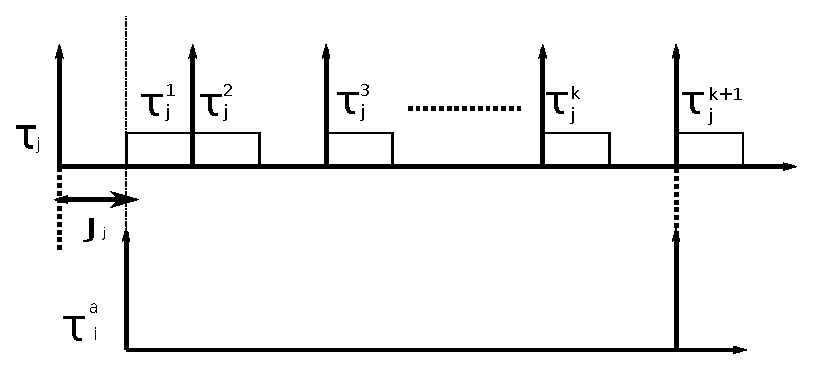
\includegraphics[bb=0bp 0bp 542bp 162bp,scale=0.5]{figures/figure1}
\par\end{centering}

\centering{}\caption{\label{fig1}Maximum interference between two tasks in G-EDF system}
\end{figure}
This can be proved by noting that $\frac{T_{i}}{T_{j}}=c.T_{j}+\delta$.
\textbf{\textit{In case $\delta\ne0$}}\textit{,} then part of an
instance of $T_{j}$ contributes in the period of $T_{i}$. If this
part is $T_{j}^{1}$, then it has a workload over $T_{i}$ because
it has a shorter absolute deadline than $T_{i}$. Otherwise, if this
part is left to the end, and the first instance of $T_{j}$ , $T_{j}^{1}$,
conincides in its release with $T_{i}$ as shown in Figure \ref{fig2},
this means that $T_{j}$ has been shifted to right, and the absolute
deadline of $T_{j}^{k}$ will be greater than that of $T_{i}$, so
it will have no effect on it, and the workload of $T_{j}$ is lowered
by one instance.

\begin{figure}
\centering{}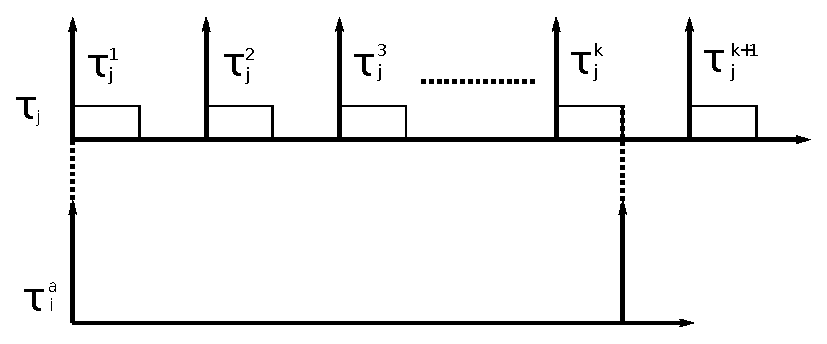
\includegraphics[scale=0.5]{figures/figure2}\caption{\label{fig2}Relase of $T_{j}^{1}$ coinciedes with $T_{i}$}
\end{figure}


If $T_{j}$ is shifted to left by any amount until the deadline of
$T_{j}^{1}$coincides with the start of $T_{i}$, this will not have
higher effect on $T_{i}$ because the deadline of $T_{j}^{k+1}$ is
still longer than that of $T_{i}$ which will make no effect for this
instance, meanwhile, it reduces the effect of $T_{j}^{1}$. This is
shown in Figure \ref{fig3}. Thus the maximum number of $T_{j}$ instances
that can interfere with $T_{i}$ in this case is $\lceil\frac{T_{i}}{T_{j}}\rceil$.

\begin{figure}
\centering{}\includegraphics[scale=0.5]{figures/figure3}\caption{\label{fig3}Deadline of $T_{j}^{1}$ coincides with $T_{i}$}
\end{figure}


\textbf{\textit{In case $\delta=0$,}} as shown in Figure \ref{fig4},
then the maximum number of $T_{j}$ instances interfering with $T_{i}$
is still $\lceil\frac{T_{i}}{T_{j}}\rceil$ because if $T_{j}^{1}$is
shifted right and delayed with jitter, it will enforce the deadline
of $T_{j}^{k}$ to exceed that of $T_{i}$, so the addition of one
instance resulted in subtraction of another. And if $T_{j}$ is shifted
left, this will not make $T_{j}^{k+1}$ has any effect on $T_{i}$
, because its absolute deadline is still longer than that of $T_{i}$,
until the deadline of $T_{j}^{k+1}$ coincides with that of $T_{i}$,
but in this case, $T_{j}^{2}$ will be removed completely from the
period of $T_{i}$, and as before, the addition of one instance resulted
in the cancelation of anoter. Then, the maximum number of interfering
instances is still the same as before.

\begin{figure}
\centering{}\includegraphics[scale=0.5]{figures/figure4}\caption{\label{fig4}$t(T_{i})$ is an integral multiple of $t(T_{j})$}
\end{figure}


This last case differs from that mentioned in \cite{key-1}, where
the maximum number of interferences is {}``$\lfloor\frac{T_{i}}{T_{j}}\rfloor+1$'',
which equals $c+1$, wherease it should be only $c$.

So, in all cases, the maximum number of instances of $T_{j}$ that
can be released during $t(T_{i})$ is 
\begin{equation}
G_{ij}(t(T_{i}))=\lceil\frac{t(T_{i})}{t(T_{j})}\rceil\label{eq1}
\end{equation}


and the maximum workload contributed by $T_{j}$ to $T_{i}$ during
the whole period of $T_{i}$ is

\begin{equation}
W_{ij}(t(T_{i}))=G_{ij}(t(T_{j})).c_{j}\label{eq8}
\end{equation}


The workload defined in \ref{eq8} is consistent with situation shown
in \ref{fig1} and may be an upper bound for the maximum workload
because in the case shown in \ref{fig9-a}, $T_{j}^{1}$ contributes
partially to $T_{i}$ rather than with all its WCET. So, a tighter
value than that of \ref{eq8} is

\begin{equation}
W_{ij}^{*}(t(T_{i}))=\lfloor\frac{t(T_{i})}{t(T_{j})}\rfloor.c_{j}+min(c_{j},t(T_{i})-\lfloor\frac{t(T_{i})}{t(T_{j})}\rfloor.t(T_{j}))\label{eq11}
\end{equation}


The bounds used in \cite{key-2} to calculate an upper bound on the
response time for EDF systems compares between three formulas to take
the minimum. The first one is useful when the calculated upper bound
is not extended to reach the last instance of the interfering task,
while the second one is used in that case because the maximum pattern
of interference of $T_{j}$ to $T_{i}$ changes according to whether
it is calculated over the whole period of $T_{i}$, or part of it.
This is illustrated in Figure \ref{fig9} where in Figure \ref{fig9-a},
the first instance $T_{j}^{1}$ can contribute partially to $T_{i}$,
but the last instance $T_{j}^{k}$ contributes by its total WCET,
this is the worst pattern of interference over $t(T_{i})$, wherease
in Figure \ref{fig9-b}, interference pattern is calculated only over
$L$, so the WCET of $T_{j}^{1}$ is totally included in the pattern,
because instances of $T_{j}^{1}$ up to $T_{j}^{k-1}$ can contribute
to the total workload over $T_{i}$ as their deadlines are shorter
than that of $T_{i}$, while in Figure \ref{fig9-a}, the inclusion
of the whole WCET of $T_{j}^{1}$ will exclude $T_{j}^{k}$ because
this will make its absolute deadline longer than that of $T_{i}$.
So, over period $L$, contribution of $T_{j}$ to $T_{i}$ is 
\begin{equation}
\hat{W}{}_{ij}(L)=(\lceil\frac{L-c_{j}}{t(T_{j})}\rceil+1).c_{j}\label{eq12}
\end{equation}
which is a little different than that mentioned in \cite{key-2} because
\cite{key-2} disscusses response time analysis for a set of feasible
tasks, but here it is not known yet whether these tasks are feasible
or not.

So, the overall workload will be
\begin{equation}
W_{ij}(L)=min(\hat{W}_{ij}(L),W_{ij}^{*}(t(T_{i})))\label{eq13}
\end{equation}


\begin{figure}
\begin{centering}
\subfloat[\label{fig9-a}]{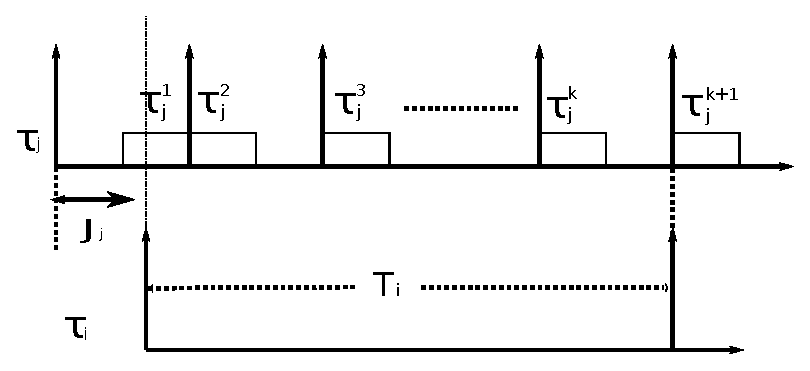
\includegraphics[scale=0.5]{figures/figure9-a}}
\par\end{centering}

\centering{}\subfloat[\label{fig9-b}]{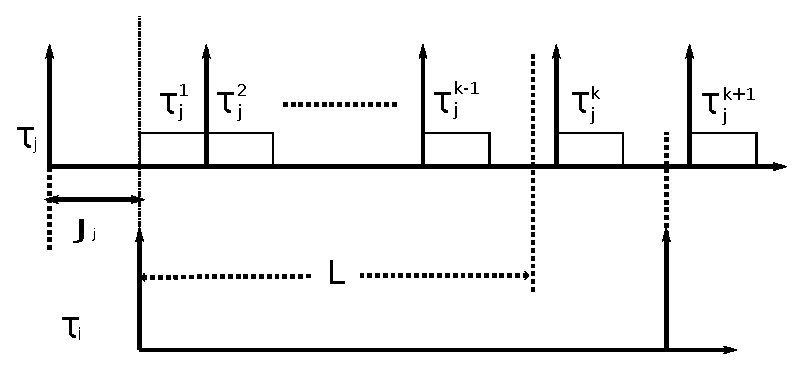
\includegraphics[scale=0.5]{figures/figure9-b}}\caption{\label{fig9}(a)Maximum interference during $t(T_{i})$ (b)Maximum
interference during part $L$ of $t(T_{i})$}
\end{figure}



\subsection{Retrial cost of atomic sections}

To get the retrial cost of any atomic section under different types
of schedulers with the specified CM, it must be noted that there are
two reasons for retrial:- 1) conflict occurs between atomic sections.
2) a task with lower priority, running on one of the processors, gets
preempted by a higher priority task while the former is executing
an atomic section. So, retrial cost of both must be calculated and
summed together.


\subsubsection{\textit{Retrial cost due to confliction between atomic sections}}

\begin{comment}
REMEMBER TO WRITE THE MORE CORRECT PROOF FOR RETRIAL OF ONE ATOMIC
SECTION DUE TO ANOTHER ATOMIC SECTION (NOT DUE TO MULTIPLE ATOMIC
SECTIONS).
\end{comment}


If there are two tasks $T_{i}$ and $T_{j}$, where the former is
of longer absolute deadline than the latter, then EDF CM will give
priority to conflicting atomic sections of $T_{j}$ over $T_{i}$
\cite{key-1}. So, an atomic section of $T_{i}$, $s_{i}^{k}(\theta)$,
will exprience its maximum dealy when it is at the end, and the one
of $T_{j}$, $s_{j}^{l}(\theta)$, is just beginning, then the CM
will enforce $s_{i}^{k}(\theta)$ to retry. Despite validation time
(i. e., eager or lazy), $s_{i}^{k}(\theta)$ will retry for the same
amount of time, which is the time of $s_{j}^{l}(\theta)$, as shown
in Figure \ref{fig5}. In Figure \ref{fig5-a}, $s_{j}^{l}(\theta)$
validates at its beginning, because of early validation, and a conflict
is detected. So, $T_{i}$ retries multiple times (because at each
start of retrial, $T_{i}$ validates) during the execution of $s_{j}^{l}(\theta)$.
When $T_{j}$ finishes its atomic section, $T_{i}$ executes its own.
In Figure \ref{fig5-b}, $T_{i}$ tries to validate at its end (because
it is lazy validation), but it finds a conflict with $T_{j}$, so
it has to retry, and beacuse its atomic section length is shorter
than that of $T_{j}$, it tries to validate again within the execution
period of $s_{j}^{l}(\theta)$, but EDF CM tells it to retry again.
This process continues until $T_{j}$ finishes its atomic section.
If $T_{i}$'s atomic section length is longer than that of $T_{j}$'s,
$T_{i}$ would have taken the same amount of tiem to retry, because
$T_{j}$ will validate when $T_{i}$ is retrying, and $T_{i}$ will
retry again as shown in Figure \ref{fig5-c}. So, the retrial cost
of $s_{i}^{k}(\theta)$ will be $len(s_{i}^{k}(\theta)+s_{j}^{l}(\theta))$.

\begin{figure}
\subfloat[\label{fig5-a}]{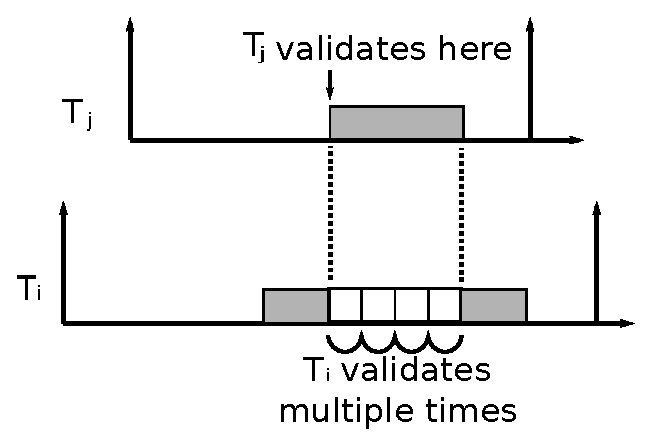
\includegraphics[scale=0.5]{figures/figure5-a}}\subfloat[\label{fig5-b}]{\qquad{}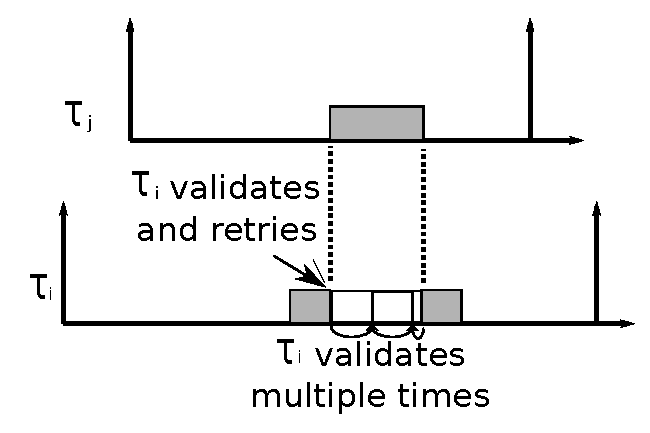
\includegraphics[scale=0.5]{figures/figure5-b}}

\centering{}\subfloat[{\small \label{fig5-c}}]{\centering{}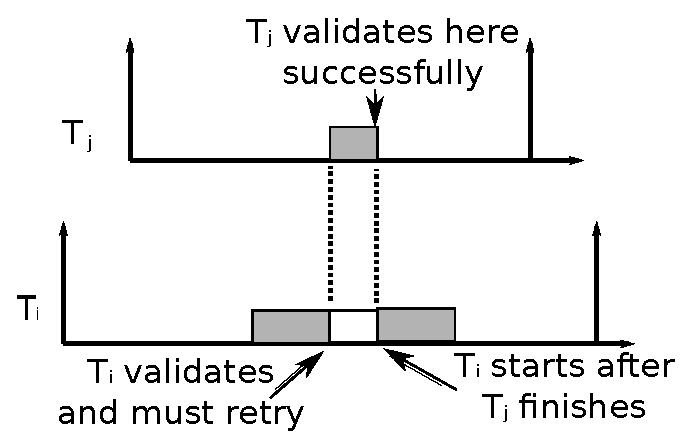
\includegraphics[scale=0.5]{figures/figure5-c}}\caption{\label{fig5}(a)Early validation (b)Lazy validation with $s_{i}^{k}(\theta)\le s_{j}^{l}(\theta)$
(c){\small Lazy validation with $s_{i}^{k}(\theta)>s_{j}^{l}(\theta)$}}
\end{figure}


But what if there are multiple tasks interfering with $T_{i}$ or
interfering with each other and $T_{i}$, as shown in Figures \ref{fig6-a},\ref{fig6-b}.
We should note that these figures are only two examples of many possible
patterns for interference between tasks and the resulting transactional
retries.

In each case, each atomic section of the shorter deadline tasks contribute
to the dealy of $s_{i}^{p}(\theta)$ by its total length, plus a retrial
to some atomic section in the longer deadline tasks. For example,
$s_{j}^{l}(\theta)$ contributes by $len(s_{j}^{l}(\theta)+s_{i}^{p}(\theta))$
in both figures, $s_{k}^{y}(\theta)$ causes a retrial to $s_{j}^{l}(\theta)$
in Figure \ref{fig6-b}, and $s_{h}^{w}(\theta)$ causes a retrial
to $s_{k}^{y}(\theta)$ in the same figure.

As it is not known in advance what atomic section will be retried
because of another one, then it can be assumed that each atomic section
(that share the same object with the studied one) in a longer deadline
task contributes by its total length, in addition to the maximum length
between all atomic sections that share the same object, $len(s_{max}(\theta))$.
\begin{equation}
\mbox{\ensuremath{W_{i}^{p}(s_{j}^{k}(\theta))=len(s_{j}^{l}(\theta)+s_{max}(\theta))}}\label{eq2}
\end{equation}


\begin{center}
\begin{figure}
\centering{}\subfloat[\label{fig6-a}]{\centering{}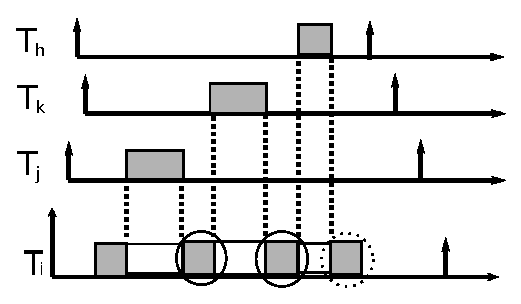
\includegraphics[scale=0.5]{figures/figure6-a}}\qquad{}\subfloat[\label{fig6-b}]{\centering{}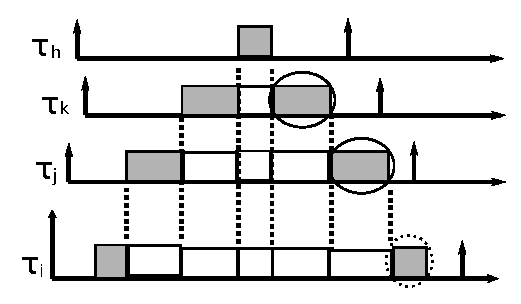
\includegraphics[scale=0.5]{figures/figure6-b}}\\%
\begin{tabular}{>{\centering}p{1.5cm}l}
\includegraphics[scale=0.5]{figures/circle} & Replaced in calculations by $s_{max}(\theta)$\tabularnewline
\includegraphics[scale=0.5]{figures/dotted_circle} & Replaced in calculations by $s_{i_{max}}(\theta)$\tabularnewline
\end{tabular}\caption{\label{fig6}(a)Other tasks interfere only with $T_{i}$ (b)All tasks
interfere with each other and $T_{i}$}
\end{figure}

\par\end{center}

So, the total contribution- of all atomic sections of all other tasks
that share objects with the studeid task- to the retrial cost of the
studied task in the period $t(T_{i})$ is 
\begin{eqnarray}
RC_{conflict}(T_{i}) & = & \sum_{\theta\in\theta_{i}}((\sum_{T_{j}\in\gamma(\theta)}(\lceil\frac{t(T_{i})}{t(T_{j})}\rceil\sum_{\forall s_{j}^{l}(\theta)\in s_{j}(\theta)}len(s_{j}^{l}(\theta)+s_{max}(\theta))))\label{eq3}\\
 &  & -s_{max}(\theta)+s_{i_{max}}(\theta))\nonumber 
\end{eqnarray}


where $\lceil\frac{T_{i}}{T_{j}}\rceil\sum_{\forall s_{j}(\theta)\in s_{j}}len(s_{j}(\theta)+s_{max}(\theta))$
referes to the contribution of all instances of $T_{j}$-as calculated
by eq(\ref{eq1}) - during the period of $T_{i}$, and this contribution
is added to all tasks. The last part in eq(\ref{eq50})- {}``$s_{i_{max}}(\theta)-s_{max}(\theta)$''-
is added because the it is known that the last atomic section to execute
is $s_{i}^{p}(\theta)$, and one of the other atomic sections (e.
g.; $s_{m}^{n}(\theta)$) should have as a contribution $len(s_{m}^{n}(\theta)+s_{i_{max}}(\theta))$
instead of $len(s_{m}^{n}(\theta)+s_{max}(\theta))$, that is why
one $s_{max}(\theta)$ is subtracted, and $s_{i_{max}}(\theta)$ is
added.

$s_{i_{max}}(\theta)$ is taken to get the worst case contribution
by all other tasks to the studied task, as one atomic section in the
latter can be interfered by more than one atomic section in any task,
but the reverse is not true, and there can be multiple atomic sections
in the studied task that share the same object.

Eq(\ref{eq50}) can be modified a little by noting that an atomic
section conflicts with the sections of other tasks, not with its own
task, because it is a hard real time sporadic model, so each instance
must finish before the next begins. So, eq(\ref{eq50}) will turn
to eq(\ref{eq4}).
\begin{eqnarray}
RC_{conflict}(T_{i}) & = & \sum_{\theta\in\theta_{i}}((\sum_{T_{j}\in\gamma(\theta)}(\lceil\frac{T_{i}}{T_{j}}\rceil\sum_{\forall s_{j}^{l}(\theta)\in s_{j}(\theta)}len(s_{j}^{l}(\theta)+s_{max}^{*}(\theta))))\label{eq4}\\
 &  & -\bar{s}_{max}(\theta)+s_{i_{max}}(\theta))\nonumber 
\end{eqnarray}


where:-
\begin{itemize}
\item $s_{max}^{*}(\theta)\in s(\theta)$ and $s_{max}^{*}(\theta)\not\in s_{j}(\theta)$
because $T_{j}$ will not cause a retrial to one of its instances.
\item To get $\bar{s}{}_{max}(\theta)$, the maximum atomic section of each
task that accesse object $\theta$ is grouped into an array of non
increasing order of their lengths, and $s_{max}(\theta)$ will be
the first one, while $\bar{s}{}_{max}(\theta)$ will be the next.
This can be illustrated by Figure \ref{fig7}, where the maximum atomic
section of each task that access object $\theta$ is associated with
its corresponding task. When eq(\ref{eq4}) is applied, all tasks
but $T_{j}$ will choose $s_{j_{max}}(\theta)$ as the value of $s_{max}^{*}(\theta)$,
as it is the maximum atomic section not assciated with the interfering
task. But when $T_{j}$ is the one whose contribution is studeid,
it will choose $s_{k_{max}}(\theta)$ as it is the maximum one not
assciated with $T_{j}$. This way, it can be seen that the maximum
value alawys lies between two values. Of course, these two values
can be equal, or the maximum value can be associated with the studeid
task itself, not with any one of the interfering tasks, in which case,
the chosen value will alawys be the one associated with the studied
task, but still the chosen value lies between the most two maximum
values. This means that the subtracted $s_{max}(\theta)$ in eq(\ref{eq50})
must be replaced with one of these two values, but as it is not known
a priori which one to use as it is not known which one will interfer
with the studied task, the minimum between them is chosen to get the
worst case retrial cost (as this value is going to be subtracted),
and this minimum is the second maximum.
\end{itemize}
\begin{center}
\begin{figure}
\begin{centering}
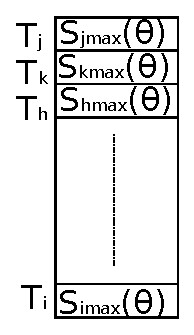
\includegraphics[scale=0.5]{figures/figure7}
\par\end{centering}

\caption{\label{fig7}Values associated with $s_{max}^{*}(\theta)$}
\end{figure}

\par\end{center}

If the maximum atomic section ($s_{i_{max}}(\theta)$) is associated
with the studeid task ($T_{i}$), then all other tasks will choose
it, and the result of eq(\ref{eq50}) for this specific object $\theta$
(i. e.; if $\theta$ is the only shared object between tasks) will
be {}``$Const+p.s_{i_{max}}(\theta)-s_{i_{max}}(\theta)+s_{i_{max}}(\theta)$'',
wherease eq(\ref{eq4}) will result in {}``$Const+p.s_{i_{max}}(\theta)-s_{k_{max}}(\theta)+s_{i_{max}}(\theta)$''
(assuming that $\bar{s}_{max}(\theta)=s_{k_{max}}(\theta)$), but
as $s_{k_{max}}(\theta)\leq s_{i_{max}}(\theta)$, then eq(\ref{eq50})
will give a smaller or equal value to eq(\ref{eq4}) for object $\theta$.

If the maximum atomic section ($s_{j_{max}}(\theta)$) is associated
with some other task ($T_{j}$), not with the studied task ($T_{i}$),
and $T_{j}$ has $n$ atomic sections that share object $\theta$,
and $\bar{s}_{max}(\theta)=s_{k_{max}}(\theta)$. Then, eq(\ref{eq50})-
for object $\theta$- will result in {}``$Const+p.s_{j_{max}}(\theta)+n.s_{j_{max}}(\theta)-s_{j_{max}}(\theta)+s_{i_{max}}(\theta)=Const+(p+n-1).s_{j_{max}}(\theta)+s_{i_{max}}(\theta)$'',
while eq(\ref{eq4}) will result in {}``$Const+p.s_{j_{max}}(\theta)+n.s_{k_{max}}(\theta)-s_{k_{max}}(\theta)+s_{i_{max}}(\theta)=Const+p.s_{j_{max}}(\theta)+(n-1).s_{k_{max}}(\theta)+s_{i_{max}}(\theta)$''.
If $n=1$, then both equations give the same result, otherwise, eq(\ref{eq4})
will give a smaller value than eq(\ref{eq50}).

It can be seen that the two equations can differ according the considered
object, but we can alawys take the minimum one for the considered
object. So, equations (\ref{eq50}) and (\ref{eq4}) can be combined
into eq(\ref{eq57}).

\begin{equation}
RC_{conflict}(T_{i})=\sum_{\theta\in\theta_{i}}min\begin{cases}
\begin{cases}
((\sum_{T_{j}\in\gamma(\theta)}(\lceil\frac{T_{i}}{T_{j}}\rceil\sum_{\forall s_{j}^{l}(\theta)\in s_{j}(\theta)}len(s_{j}^{l}(\theta)+s_{max}(\theta))))\\
-s_{max}(\theta)+s_{i_{max}}(\theta))
\end{cases}\\
\\
\begin{cases}
((\sum_{T_{j}\in\gamma(\theta)}(\lceil\frac{T_{i}}{T_{j}}\rceil\sum_{\forall s_{j}^{l}(\theta)\in s_{j}(\theta)}len(s_{j}^{l}(\theta)+s_{max}^{*}(\theta))))\\
-\bar{s}_{max}(\theta)+s_{i_{max}}(\theta))
\end{cases}\\
\\
\end{cases}\label{eq5}
\end{equation}



\subsubsection{\textit{Retrial cost due to preemption by higher priority tasks}}

When the studeid job ($\tau_{i}^{x}$) has a long absolute deadline
among all tasks running on the $m$ processors, and another job ($\tau_{j}^{l}$)
is released $d_{j}^{l}<d_{i}^{x}$, then $\tau_{i}^{x}$ will be preempted
in favor of $\tau_{j}^{l}$, but this can happen when $\tau_{i}^{x}$
is at the end of one of its atomic sections, which will enforce it
to retry- despite there is no conflict . This situation is illustrated
in Figure \ref{fig8}.

Generally, for any instance $\tau_{j}^{l}$ to be able to preempt
$\tau_{i}^{x}$, then two conditions must be satisfied: $r_{i}^{x}<r_{j}^{l}<d_{i}^{x}$,
and $d_{j}^{l}\le d_{i}^{x}$. Wihout the first condition, $\tau_{j}^{l}$
would have been released already before $\tau_{i}^{x}$ and it will
not preempt it. Without the second condition, $\tau_{j}^{l}$ will
be of lower priority than $\tau_{i}^{x}$ and will not preempt it.
So, If $D_{j}\ge D_{i}$, then no instance of $\tau_{j}$ will preempt
$\tau_{i}^{x}$because there will be at most one instance of $\tau_{j}$
with higher priority than $\tau_{i}^{x}$, and this instance must
have been released before $\tau_{i}^{x}$, which violates the first
condition. Otherwise, this instance will be of lower priority than
$\tau_{i}^{x}$, which violates the second condition.

So, to get the $RC_{release}$ of any instance of $\tau_{i}$ during
an interval $L\le T_{i}$, only tasks with shorter relative deadline
than $D_{i}$ are going to be considered as shown in eq(\ref{eq6}).

\begin{equation}
RC_{release}(L)=\sum_{\tau_{j}\in\zeta_{i}}\begin{cases}
\left\lceil \frac{L}{T_{j}}\right\rceil s_{i_{max}} & ,L\le T_{i}-T_{j}\\
\left\lfloor \frac{T_{i}}{T_{j}}\right\rfloor s_{i_{max}} & ,L>T_{i}-T_{j}
\end{cases}\label{eq6}
\end{equation}
where $\zeta_{i}$ is the set of tasks with relative deadline shorter
than $D_{i}$, and $s_{i_{max}}$ is the longest transaction in $\tau_{i}$
as it is assumed that $\tau_{j}^{l}$ preempts $\tau_{i}^{x}$ when
it is executing $s_{i_{max}}$ to get the worst case scenario.

Although the total number of instances of $\tau_{j}$ that are released
during any interval $L\le T_{i}$ is $\left\lceil \frac{L}{T_{i}}\right\rceil +1$,
but for the case of G-EDF, carried-in and carried-out jobs are discarded
because carried-in jobs are released before $r_{i}^{x}$, which violates
the first condition mentioned above, while carried-out jobs are of
lower priority than $\tau_{i}^{x}$, which violates the second condition.
This is why ceiling is used in the first case of (\ref{eq6}) and
floor is used in the second case.

\begin{figure}
\centering{}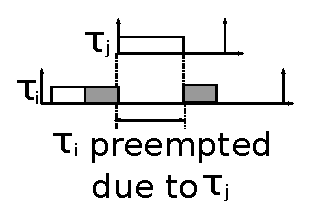
\includegraphics[scale=0.7]{figures/figure8}\caption{\label{fig8}Transactional retries due to release of higher priority
tasks}
\end{figure}


So, the total retrial cost of $T_{i}$ will be

\begin{equation}
RC(T_{i})=RC_{conflict}(T_{i})+RC_{release}(T_{i})\label{eq7}
\end{equation}



\subsection{Upper bound on response time}

To get an upper bound on the response time of $T_{i}$, $RC(T_{i})$
must be added to the workload by other tasks during the non-atomic
execution of $T_{i}$. But this requires modification of WCET of each
task as follows:-

WCET ($c_{j}$) of each interfering task ($T_{j}$) should be inflated
to accomodate for the interference of tasks other than the studied
one ($T_{k},$ $k\ne j,i$), meanwhile, atomic region that access
shared objects between $T_{j}$ and $T_{i}$ should not be considered
in the inflation cost becuase they are already calculated in the retrial
cost of the studied task ($T_{i}$). So, the new WCET for $T_{j}$
will be

\begin{equation}
c_{ji}=c_{j}-\sum_{\theta\in(\theta_{j}\wedge\theta_{i})}len(s_{j}(\theta))+RC_{conflict}(T_{ji})+RC_{releas}(T_{ji})\label{eq9}
\end{equation}


where:-

$c_{ji}$ is the new WCET of $T_{j}$ relative to the studied task
$T_{i}$. This length changes according to the studied task.

$len(s_{j}(\theta))$ is the sum of lengths of all atomic sections
in $T_{j}$ that access object $\theta$.

$RC_{conflict}(T_{ji})$ is calculated as in \ref{eq57} without including
shared objects between $T_{i}$ and $T_{j}$.

$RC_{release}(T_{ji})$ is calculated as in \ref{eq6} without considering
the release of any instance of $T_{i}$.

The second term in \ref{eq9} is included because the length of these
atomic sections is already included in the retrial cost of $T_{i}$,
so as in the third term. The last term excludes any release of any
instance of $T_{i}$ because it is assumed that $T_{j}$ is the one
that affects $T_{i}$, not the reverse. Because of this, the calculated
WCET is relative to the studied task, as it changes form task to task.

So, the upper bound on the response time of $T_{i}$ will be calculated
by the iterative equation (which is modified from theorm 6 in \cite{key-2}):-

\begin{equation}
R_{i}^{up}=c_{i}+RC(T_{i})+\lfloor\frac{1}{m}\sum_{j\ne i}W_{ij}(R_{i}^{up})\rfloor\label{eq10}
\end{equation}


where:-

$R_{i}^{up}$ is the iterative calculated upper bound on the response
time of $T_{i}$, and its initial value is $c_{i}+RC(T_{i})$.

$W_{ij}(R_{i}^{up})$ is calculated by \ref{eq13}, but $W_{ij}^{*}(t(T_{i}))$
will be calculated by eq(\ref{eq11}) with replacing $c_{j}$ with
$c_{ji}$, and $\hat{W}_{ij}(L)$ will be changed to 
\begin{equation}
\hat{W}_{ij}(L(T_{i}))=max\begin{cases}
(\lceil\frac{L-c_{ji}-\sum_{\theta\in(\theta_{j}\wedge\theta_{i})}len(s_{j}(\theta))}{t(T_{j})}\rceil+1).c_{ji}\\
\lceil\frac{L-c_{j}}{t(T_{j})}\rceil.c_{ji}+c_{j}-\sum_{\theta\in(\theta_{j}\wedge\theta_{i})}len(s_{j}(\theta))
\end{cases}\label{eq14}
\end{equation}
where the top term is the same as that calculated by eq(\ref{eq12})
but with replacing $c_{j}$ with $c_{ji}$ and addition of legnths
of atomic sections shared between $T_{i}$ and $T_{j}$. Although
these lengths are already included in the retrial cost of $T_{i}$,
but they are added here to get an approximate right start time for
other instances of $T_{j}$ that affect $T_{i}$. It is approximate
because the added atomic sections are not subject to retrial by other
tasks (because the retrial is included in $RC(T_{i})$), but calculations
are still valid because inclusion of retrial to these sections will
reduce the output of the ceiling in the top term, so it still gives
a maximum value. 

The lower term in eq(\ref{eq14}) does the same except for the first
instance of $T_{j}$ which contributes by only $c_{j}$, and the shared
atomic sections between $T_{i}$ and $T_{j}$ are excluded from this
first instance.

These two terms are compared becuase $\lceil\frac{L-c_{j}}{t(T_{j})}\rceil.c_{ji}>\lceil\frac{L-c_{ji}}{t(T_{j})}\rceil.c_{ji}$
but $c_{ji}>c_{j}$, this makes a tradeoff beween these two terms,
so the maximum is chosen.


\subsubsection{Tighter upper bound on response time}

To get a tighter upper bound on response time of $T_{i}$, the $RC(T_{i})$
will not be fixed (as is done in eq(\ref{eq10}) because it is calculated
over the entire period of $T_{i}$), rather it will change according
to $R_{i}^{up}$. So, eq(\ref{eq57}) will be changed to include the
modified number of interfering instances in the same way this number
is calculated in eq(\ref{eq13}), but when calculating this number
for the entire $t(T_{i})$, a situation like that shown in Figure
\ref{fig10} can happen.
\begin{figure}
\centering{}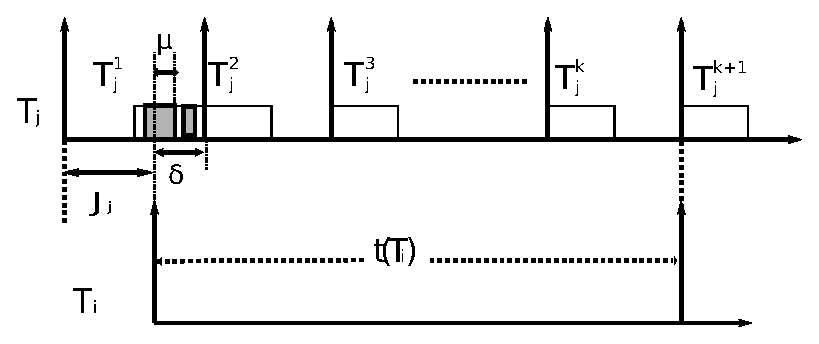
\includegraphics[scale=0.5]{figures/figure10}\caption{\label{fig10}Atomic sections of $T_{j}^{1}$ contributing to }
\end{figure}
Atomic sections of $T_{j}^{1}$ that are contained in period $\delta$
are the only ones that at most can contribute to the $RC(T_{i})$,
of course they can be lower, but cannot be greater because $T_{j}^{1}$
has been delayed by its maximum jitter, so no more atomic sections
can enter period $[d(T_{j}^{1})-\delta,d(T_{j}^{1})]$. Besides, $T_{i}$
can be released in the middle of any atomic section that shares an
object with it, so only length $\mu$ of this atomic section will
be considered, but the effect of this $\mu$ will still be the retrial
of one of the other atomic sections. So, eq(\ref{eq57}) will be modified
as shown in eq(\ref{eq52}).

\begin{equation}
RC_{conflict}(t(T_{i}))=\sum_{\theta\in\theta_{i}}min\begin{cases}
\begin{cases}
((\sum_{T_{j}\in\gamma(\theta)}(\sum_{\forall s_{j}^{l}(\theta)\in[d(T_{j}^{1})-\delta,d(T_{j}^{1}))]^{*}}len(s_{j}^{l^{*}}(\theta)+s_{max}(\theta)))+\\
(\lceil\frac{t(T_{i})}{t(T_{j})}\rceil\sum_{\forall s_{j}^{l}(\theta)\in s_{j}(\theta)}len(s_{j}^{l}(\theta)+s_{max}(\theta))))-s_{max}(\theta)+s_{i_{max}}(\theta))
\end{cases}\\
\\
\begin{cases}
((\sum_{T_{j}\in\gamma(\theta)}(\sum_{\forall s_{j}^{l}(\theta)\in[d(T_{j}^{1})-\delta,d(T_{j}^{1}))]^{*}}len(s_{j}^{l^{*}}(\theta)+s_{max}^{*}(\theta)))+\\
(\lceil\frac{t(T_{i})}{t(T_{j})}\rceil\sum_{\forall s_{j}^{l}(\theta)\in s_{j}(\theta)}len(s_{j}^{l}(\theta)+s_{max}^{*}(\theta))))-\bar{s}_{max}(\theta)+s_{i_{max}}(\theta))
\end{cases}\\
\\
\end{cases}\label{eq15}
\end{equation}


where:-

$s_{j}^{l^{*}}(\theta)$ is the part of $s_{j}^{l}(\theta)$ that
is included in $[d(T_{j}^{1})-\delta,d(T_{j}^{1}))]$.

$[d(T_{j}^{1})-\delta,d(T_{j}^{1}))]^{*}$ contains $s_{j}^{l}(\theta)$
if it is partially or totaly included in it. In the latter case, $s_{j}^{l}(\theta)$
will contribute by its included length $\mu$.

Now, it is time to compute $RC_{conflict}(T_{i})$ during a period
of length $L$ which does not extend to the last instance of $T_{j}$.
In this case, eq(\ref{eq57}) will be (\ref{eq16}) .

\begin{equation}
RC_{conflict}(L(T_{i}))=\sum_{\theta\in\theta_{i}}min\begin{cases}
\begin{cases}
((\sum_{T_{j}\in\gamma(\theta)}((\lceil\frac{L-c_{j}}{t(T_{j})}\rceil+1)\sum_{\forall s_{j}^{l}(\theta)\in s_{j}(\theta)}len(s_{j}^{l}(\theta)\\
+s_{max}(\theta))))-s_{max}(\theta)+s_{i_{max}}(\theta))
\end{cases}\\
\begin{cases}
((\sum_{T_{j}\in\gamma(\theta)}((\lceil\frac{L-c_{j}}{t(T_{j})}\rceil+1)\sum_{\forall s_{j}^{l}(\theta)\in s_{j}(\theta)}len(s_{j}^{l}(\theta)\\
+s_{max}^{*}(\theta))))-\bar{s}_{max}(\theta)+s_{i_{max}}(\theta))
\end{cases}
\end{cases}\label{eq16}
\end{equation}


So, $RC_{conflict}$ during the upper bound on the response time of
$T_{i}$ can be calculated as in eq(\ref{eq17})

\begin{equation}
RC_{conflict}(R_{i}^{up})=min\begin{cases}
RC_{conflict}(R_{i}^{up}(T_{i}))\\
RC_{conflict}(t(T_{i}))
\end{cases}\label{eq17}
\end{equation}


\textbf{$RC_{release}(T_{i})$} is also modified to eq(\ref{eq18}).

\begin{equation}
RC_{release}(R_{i}^{up})=\sum_{T_{k}\in\zeta(T_{i})}(\lfloor\frac{R_{i}}{T_{k}}\rfloor.s_{i_{max}}(\theta))\label{eq18}
\end{equation}


and the final retrial cost of $T_{i}$ will be calculated in eq(\ref{eq19})

\begin{equation}
RC(R_{i}^{up})=RC_{conflict}(R_{i}^{up})+RC_{release}(R_{i}^{up})\label{eq19}
\end{equation}


So, the final upper bound on response time of $T_{i}$ will be calculated
as in eq(\ref{eq10}) with replacing $RC_{conflict}(T_{i})$ with
$RC(R_{i}^{up})$.


\section{Response time of G-RMA system with RMA CM}

As G-RMA is a fixed scheduler, $T_{i}$ will be interfered by a specific
set of tasks whose priorities are higher than or equal to that of
$T_{i}$ ($p(T_{j})\ge p(T_{i})$).


\subsection{Maximum Interference of tasks with G-RMA scheduler}

Figure \ref{fig11} represents the maximum interference of $T_{j}$
to $T_{i}$ under G-RMA. As $T_{j}$ is of higher priority than $T_{i}$,
then $T_{j}^{k}$ will interfere with $T_{i}$ even if it is not totally
included in $t(T_{i})$. Unlike the G-EDF case shown in Figure \ref{fig10}
where only the $\delta$ part of $T_{j}^{1}$ is considered, in G-RMA,
$T_{j}^{k}$ will contribute with the whole $c_{j}$ and all atomic
sections contained in $T_{j}^{k}$ will be considered. This is becasue
in G-EDF, the worst case pattern releases $T_{i}$ before $d(T_{j}^{1})$
by$\delta$ time units, and $T_{i}$ cannot be interfered before it
is released, but in G-RMA, $T_{i}$ is already released, and can be
interfered by the whole $T_{j}^{k}$ even if this is going to render
it infeasible.

So, the maximum contribution of $T_{j}$ to $T_{i}$ for any period
$L$ can be deduced from Figure \ref{fig11} as $W_{ij}(L(T_{i}))=(\lceil\frac{L-c_{j}}{t(T_{j})}\rceil+1).c_{j}$,
where $L$ can extend to $t(T_{i})$, and not like the case of G-EDF
where the pattern of interference is different for each interval.

\begin{figure}
\centering{}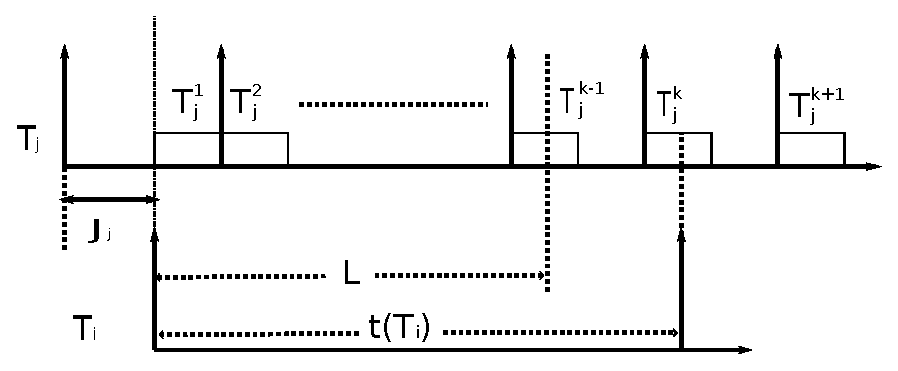
\includegraphics[scale=0.5]{figures/figure11}\caption{\label{fig11}Maximum interference of $T_{j}$ to $T_{i}$ in G-RMA}
\end{figure}



\subsection{Retrial cost due to conflict between atomic sections}

Eq(\ref{eq20}) is used to calculate the retrial cost due to conflict
between atomic sections. It is the same as eq(\ref{eq16}) with some
modifications as we do not have get the minimum of two formulas, because
any atomic section in $T_{j}$ will cause retrial to one of the atomic
sections in lower or equal priority tasks; that is why $s_{max}^{j}(\theta)$
is used. Also, only tasks of higher or equal priority to $T_{i}$
are considered as they are the only ones to interfere with it.

\begin{eqnarray}
RC_{conflict}(L(T_{i})) & = & \sum_{\theta\in\theta_{i}}((\sum_{(T_{j}\in\gamma(\theta))\wedge(p(T_{j})\ge p(T_{i}))}((\lceil\frac{L-c_{j}}{t(T_{j})}\rceil+1).\label{eq20}\\
 &  & \sum_{\forall s_{j}^{l}(\theta)}len(s_{j}^{l}(\theta)+s_{max}^{j}(\theta))))-s_{max}^{j}(\theta)+s_{i_{max}}(\theta))\nonumber 
\end{eqnarray}


$L(T_{i})$ can be extended to $t(T_{i})$ because of the fixed priority.


\subsection{Retrial cost due to release of higher priority tasks}

Eq(\ref{eq18}) can be modified to get the retrial cost due to release
of higher priority tasks. 

\begin{equation}
RC_{release}(L(T_{i}))=\sum_{p(T_{k})\ge p(T_{i})}(\lceil\frac{L}{T_{k}}\rceil.s_{i_{max}}(\theta))\label{eq21}
\end{equation}
The interval $L$ in eq(\ref{eq20}) can be extended to cover the
whole period of $t(T_{i})$. So, the total retrial cost of $T_{i}$
($RC(R_{i}^{up})$) can be calculated as in eq(\ref{eq19}).


\subsection{Upper bound on response time}

Upper bound can be calculated by eq(\ref{eq22})
\begin{equation}
R_{i}^{up}=c_{i}+RC(R_{i}^{up})+\lfloor\frac{1}{m}\sum_{j\ne i}\hat{W}{}_{ij}(R_{i}^{up})\rfloor\label{eq22}
\end{equation}
where $\hat{W}_{ij}(R_{i}^{up})$ is calculated as in eq(\ref{eq14})
and $c_{ji}$ is calculated by eq(\ref{eq9}) but $RC_{conflict}(T_{i})$
and $RC_{release}(T_{i})$ are calculated by eq(\ref{eq20}) and (\ref{eq21})
respectively.


\section{\label{sec:Response-time-of FIFO CM}Response time of G-EDF and G-RMA
system with FIFO CM}

In FIFO CM, transactions are executed in the order they arrive. This
way, the effect of an atomic section of $T_{j}$ to one in $T_{i}$
is shown in Figure \ref{fig12-a} for early validation and Figure
\ref{fig12-b} for lazy validation. In both cases, $s_{i}^{l}(\theta)$
must retry for at most $len(s_{j}^{p}(\theta))$, which is less than
that of EDF CM and RMA CM, but a higher priority task can be delayed
by a lower one if the latter's atomic section arrives earlier than
the former.

\begin{figure}
\centering{}\subfloat[\label{fig12-a}]{\centering{}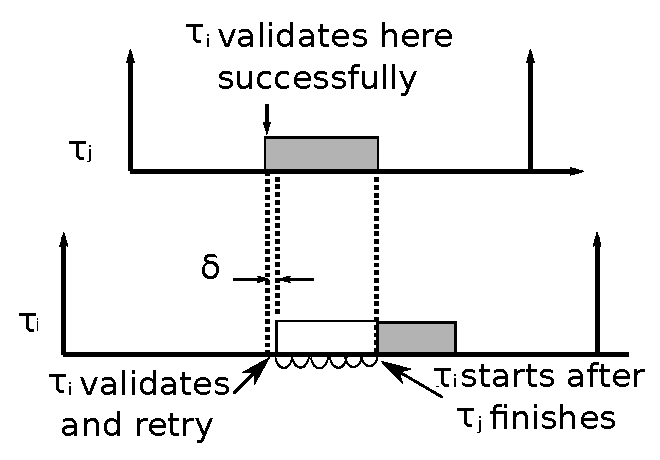
\includegraphics[scale=0.5]{figures/figure12-a}}\subfloat[\label{fig12-b}]{\centering{}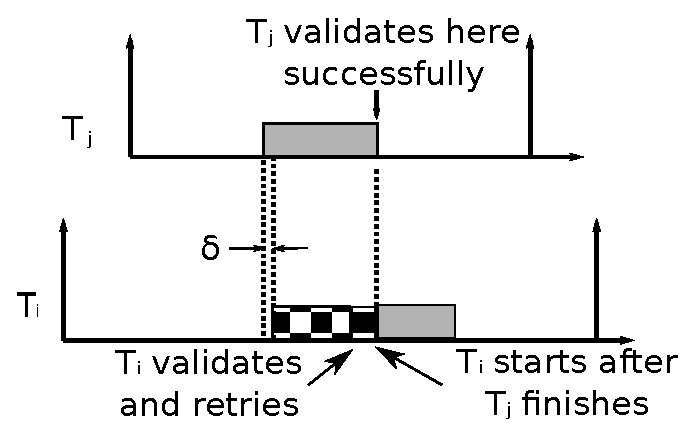
\includegraphics[scale=0.5]{figures/figure12-b}}\caption{\label{fig12}(a)Early validation (b)Lazy validation}
\end{figure}


Retrial of atomic sections here does not depend on the scheduler,
rather it only depends on the arrival pattern, so conflict retrial
cost ($RC_{conflict}$) will be the same for both G-EDF and G-RMA
systems, and the maximum pattern of interference will also be the
same as shown in Figure \ref{fig11}, but this pattern differs when
calculating the release retrial cost ($RC_{release}$) and the contribution
of other tasks during the non-atomic part of $T_{i}$.

$RC_{conflict}$ can be calculated by eq(\ref{eq23})
\begin{equation}
RC_{conflict}(L(T_{i}))=\sum_{\theta\in\theta_{i}}((\sum_{T_{j}\in\gamma(\theta)}((\lceil\frac{L-c_{j}}{t(T_{j})}\rceil+1).\sum_{\forall s_{j}^{l}(\theta)}len(s_{j}^{l}(\theta)))))\label{eq23}
\end{equation}
where the lengths of all atomic sections in all tasks that share object
$\theta$ with $T_{i}$ are summed together, and $L$ can extend to
cover $t(T_{i})$. It should be noted that one instance can have multiple
atomic sections that access the same object, then how can an atomic
section of $T_{i}$ be interfered by all of them while it should be
interfered by only one of them according to its arrival time, the
others will come after that of $T_{i}$? This can happen if $T_{i}$
was trying to execute its atomic section, then it is replaced by a
higher priority job, then $T_{i}$ gets back to the processor. In
the time of preemption, another atomic section of the same conflicting
task can come and execute. This situation is shown in Figure \ref{fig13}
where $s_{i}^{l}$ retries while $s_{j}^{p}$ is executing, then $T_{k}$
is released, preempting $T_{i}$ to get its processor and before it
finished, $s_{j}^{p+1}$ executes, so when $s_{i}^{l}$ returns after
$T_{k}$ finishes, it will be after $s_{j}^{p+1}$ and it will have
to retry until it finishes. For this, eq(\ref{eq23}) sums the lengths
of all atomic sections in each instance that access the same object
as the studeid task.

\begin{figure}
\centering{}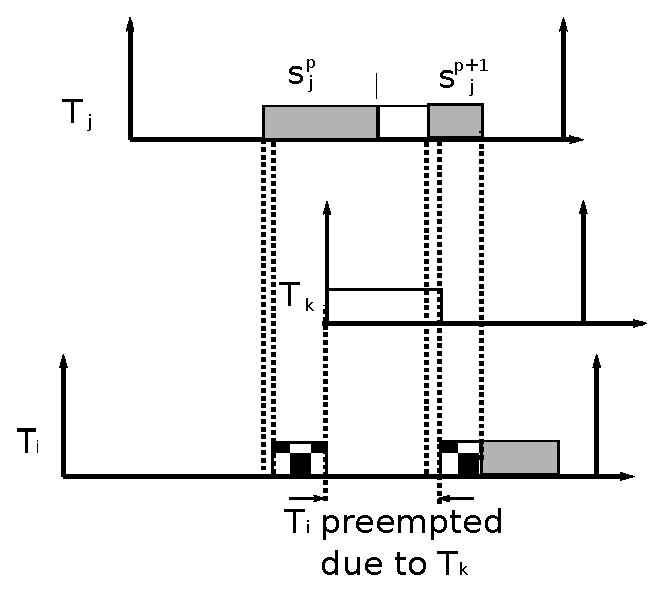
\includegraphics[scale=0.5]{figures/figure13}\caption{\label{fig13}Retrial of $s_{i}^{l}$ by multiple atomic sections
of $s_{j}^{p}$}
\end{figure}


The rest of analysis for both schedulers is done as before, only $RC_{conflict}(L(T_{i}))$
is changed.


\subsection{\textmd{In case of G-RMA}}

$RC_{conflict}$ can be reduced for G-RMA by noting that the case
shown in Figure \ref{fig13} can happen only if $T_{i}$ is the lowest
priority among all running tasks, which reduces number of conflicting
tasks to only those of higher or equal priority to that of $T_{i}$.
Meanwhile, if there are $m$ processors, this means that before $T_{i}$
gets preempted, it will retry for the duration of at most the maximum
$m-1$ atomic sections sharing the same object with $T_{i}$.

After $T_{i}$ gets preempted, no lower priority task can allocate
a processor while $T_{i}$ is waiting, but as $T_{i}$ can get preempted
again and again by higher priority tasks, it can be delayed by the
sum of all atomic sections in higher priority tasks that access the
same object as $T_{i}$, or for each release of a higher priority
job, $T_{i}$ will be delayed by the maximum $m-1$ higher or equal
priority tasks

So, $RC_{conflict}$ in the case of G-RMA can be calculated as in
eq(\ref{eq24})

\begin{eqnarray}
RC_{conflict}(L(T_{i}))= & \sum_{\theta\in\theta_{i}}(\sum_{k=1}^{min(n-1,m-1)}(\omega(k,\theta))+(\sum_{(T_{j}\in\gamma(\theta))\wedge(p(T_{j})\ge p(T_{i}))}min((\lceil\frac{L}{t(T_{j})}\rceil).\label{eq24}\\
 & \sum_{k=1}^{m-1}(\omega_{high}(k,\theta)),((\lceil\frac{L-c_{j}}{t(T_{j})}\rceil+1).\sum_{\forall s_{j}^{l}(\theta)}len(s_{j}^{l}(\theta)))))_{0\, if\, n\le m})\nonumber 
\end{eqnarray}


where:-

$\omega(k,\theta)$ is the set of $s_{p_{max}}(\theta)$ arranged
in non-increasing order. 

$\omega_{high}(k,\theta)$ is the set of $s_{p_{max}}(\theta)$ arranged
in non-increasing order, where $p(T_{p})\ge p(T_{i})$. 

The second term is zero in case number of tasks is less than or equal
to number of processors, because $T_{i}$ will not have to be preempted
because of enough number of processors for tasks. The rest of the
analysis for $RC_{releas}$ and workload of other tasks is the same.


\subsection{\textmd{In case of G-EDF}}

G-EDF is similar to G-RMA in that $T_{i}$- before it is preempted-
it can be delayed by the maximum $min(m-1,n-1)$ tasks, but when if
it is preempted, this means that $T_{i}$ is the least priority task
and all other $m-1$ tasks are of higher or equal priority, and $T_{i}$-
or one of higher or equal priority- is allowed to allocate a processor
when one is available, so no $T_{j}$ of longer relative deadline
than $T_{i}$ will start before it because it will have a longer absolute
deadline. So, $RC_{conflict}$ in the case of G-EDF will be calculated
as shown in eq(\ref{eq24}) where $L$ can be extended to $t(T_{i})$.

\begin{eqnarray}
RC_{conflict}(L(T_{i}))= & \sum_{\theta\in\theta_{i}}(\sum_{k=1}^{min(n-1,m-1)}(\omega(k,\theta))+(\sum_{(T_{j}\in\gamma(\theta))\wedge(D(T_{j})\le D(T_{i}))}min((\lfloor\frac{L}{t(T_{j})}\rfloor).\nonumber \\
 & \sum_{k=1}^{m-1}(\omega_{high}(k,\theta)),(min[\lceil\frac{L-c_{j}}{t(T_{j})}\rceil+1,\lfloor\frac{t(T_{i})}{t(T_{j})}\rfloor].\sum_{\forall s_{j}^{l}(\theta)}len(s_{j}^{l}(\theta)))))_{0\, if\, n\le m}) & \text{}\label{eq25}
\end{eqnarray}


$RC_{release}$ and workload of other tasks is the same as before.


\section{Comparison between different synchronization approaches}


\subsection{Comparison between EDF CM, RMA CM and FIFO CM}

In both EDF CM and RMA CM, any atomic section $s_{i}^{l}$ can suffer
from retrial cost of $len(s_{i}^{l}+s_{j}^{k})$ from an interfering
task $T_{j}$, whereas, FIFO CM suffers only from $len(s_{j}^{k})$.

In case of G-RMA scheduler, both RMA CM and FIFO CM suffer from higher
priority tasks (although the latter suffers from $min(m-1,n-1)$ tasks,
but due to preemption by higher priority tasks, it can be affected
by all of them as depicted in (\ref{eq24})) and any task $T_{i}$
is interfered by the same number of instances of $T_{j}$ for both
approaches (this number can extend to the carry out job during the
whole period of $T_{i}$), but FIFO CM initially suffers from $m-1$
tasks that have their atomic sections ordered in the queue before
it.

EDF CM is somehow similar to FIFO CM in that it initially suffers
from all tasks, even those with longer relative deadline, because
they may have shorter or equal aboslute deadline, but afterwards,
it can suffer from those of shorter relative deadline if their coming
instances still have shorter absolute deadline during the period of
the studied task; in that it differs from RMA CM which is affected
only by the higher priority tasks, but EDF CM is not affected by carry
out instances, so a task $T_{i}$ may be interfereb by a lower number
of instances of $T_{j}$.

So, it can be seen that the major factors that differentiate the three
contention managers are:- the number of interfering tasks, which in
turn is affected by the priority of the task, and the number of instances
of any conflicting task.


\subsection{Comparison between lock-free and STM}

In order to know when the previously mentioned STM systems are better
than lock free approach, we follow the comparison made in \cite{key-1}
by comparing the total utilization of each one. Lock free method is
implemented using retrial loops \cite{key-5}. In each approach, execution
time of each task is inflated by the retrial cost (in case of STM),
or the loop retrial cost (in case of lock free).


\subsubsection{\label{sub:G-EDF-scheduler-with}G-EDF scheduler with EDF CM against
lock-free}

Equation (\ref{eq17}) can be upper bounded by (\ref{eq30})
\begin{equation}
RC(T_{i})=\sum_{T_{j}\in\gamma_{i}}(\sum_{\theta\in\theta_{i}}(\lceil\frac{t(T_{i})}{t(T_{j})}\rceil\sum_{\forall s_{j}^{l}(\theta)}(2.s_{max})))\label{eq30}
\end{equation}
where $s_{j}^{l}(\theta)$, $s_{max}(\theta)$, $s_{i_{max}}(\theta)$,
$s_{max}^{*}(\theta)$ and $\bar{s}_{max}(\theta)$ are replaced by
$s_{max}$, and the order of the first two summation are replaced
by each other with $\gamma_{i}$ is the set of tasks that share objects
with $T_{i}$. These two changes are done to simplify the comparison,
in addition to assuming that $\sum_{\theta\in\theta_{i}}\sum_{\forall s_{j}^{l}(\theta)}=\beta_{i,j}^{*}$.
So, (\ref{eq30}) can be modified to (\ref{eq31})
\begin{equation}
RC(T_{i})=\sum_{T_{j}\in\gamma_{i}}\lceil\frac{t(T_{i})}{t(T_{j})}\rceil.2\beta_{i,j}^{*}.s_{max}\label{eq31}
\end{equation}
The loop retrial cost is defined in \cite{key-5} as (\ref{eq33})
\begin{equation}
\sum_{T_{j}\in\gamma_{i}}(\lceil\frac{t(T_{i})}{t(T_{j})}\rceil+1).\beta_{i,j}.r_{max}\label{eq32}
\end{equation}
where $\beta_{i,j}$ is number of retry loops of $T_{j}$ that access
the same object as accessed by some retry loop of $T_{i}$, but as
the shared objects are the same in both STM and lock free, so $\beta_{i,j}=\beta_{i,j}^{*}$,
and $r_{max}$ is the maximum execution cost of a single iteration
of any retry loop of any task.

\begin{flushleft}
So, STM acheives better or equal performance to lock-free if the total
utilization of the former is less than or equal to the latter as shown
in (\ref{eq33})
\begin{eqnarray}
\sum_{T_{i}}\frac{c_{i}+\sum_{T_{j}\in\gamma_{i}}\lceil\frac{t(T_{i})}{t(T_{j})}\rceil.2\beta_{i,j}.s_{max}}{t(T_{i})} & \le & \sum_{T_{i}}\frac{c_{i}+\sum_{T_{j}\in\gamma_{i}}(\lceil\frac{t(T_{i})}{t(T_{j})}\rceil+1).\beta_{i,j}.r_{max}}{t(T_{i})}\nonumber \\
\therefore\frac{s_{max}}{r_{max}} & \le & \frac{\sum_{T_{i}}(\sum_{T_{j}\in\gamma_{i}}(\lceil\frac{t(T_{i})}{t(T_{j})}\rceil+1).\beta_{i,j})/t(T_{i})}{\sum_{T_{i}}(\sum_{T_{j}\in\gamma_{i}}\lceil\frac{t(T_{i})}{t(T_{j})}\rceil.2\beta_{i,j})/t(T_{i})}\nonumber \\
 & = & \frac{\sum_{T_{i}}(\sum_{T_{j}\in\gamma_{i}}\lceil\frac{t(T_{i})}{t(T_{j})}\rceil.\beta_{i,j})/t(T_{i})}{2\sum_{T_{i}}(\sum_{T_{j}\in\gamma_{i}}\lceil\frac{t(T_{i})}{t(T_{j})}\rceil.\beta_{i,j})/t(T_{i})}+\frac{\sum_{T_{i}}(\sum_{T_{j}\in\gamma_{i}}\beta_{i,j})/t(T_{i})}{2\sum_{T_{i}}(\sum_{T_{j}\in\gamma_{i}}\lceil\frac{t(T_{i})}{t(T_{j})}\rceil.\beta_{i,j})/t(T_{i})}\nonumber \\
 & = & \frac{1}{2}+\frac{\sum_{T_{i}}(\sum_{T_{j}\in\gamma_{i}}\beta_{i,j})/t(T_{i})}{2\sum_{T_{i}}(\sum_{T_{j}\in\gamma_{i}}\lceil\frac{t(T_{i})}{t(T_{j})}\rceil.\beta_{i,j})/t(T_{i})}\label{eq33}
\end{eqnarray}
Let $\zeta_{1}=\sum_{T_{i}}(\sum_{T_{j}\in\gamma_{i}}\beta_{i,j})/t(T_{i})$
and $\zeta_{2}=\sum_{T_{i}}(\sum_{T_{j}\in\gamma_{i}}\lceil\frac{t(T_{i})}{t(T_{j})}\rceil.\beta_{i,j})/t(T_{i})$,
$\therefore\,\zeta_{1}\le\zeta_{2}$ depending on $\lceil\frac{t(T_{i})}{t(T_{j})}\rceil$,
and the maximum value of $\frac{\zeta_{1}}{2.\zeta_{2}}=\frac{1}{2}$
which can happen if $t(T_{j})\ge t(T_{i})\,\therefore\lceil\frac{t(T_{i})}{t(T_{j})}\rceil=1$,
and $(\ref{eq33})=1$ which is its maximum value. Of course, $t(T_{j})\ge t(T_{i})$
means that there is small number of interferences from other tasks
to $T_{i}$, consequently, low number of conflict, so $s_{max}$ is
allowed to be as large as $r_{max}$.
\par\end{flushleft}

The theoritical minimum value for $\frac{\zeta_{1}}{2.\zeta_{2}}$
is $0$ which can be asymptotically reached if $t(T_{j})\ll t(T_{i})$,
$\therefore\,\lceil\frac{t(T_{i})}{t(T_{j})}\rceil\rightarrow\infty$
and $\zeta_{2}\rightarrow\infty$, so $(\ref{eq33})\rightarrow1/2$.

So, it can be seen that $\beta_{i,j}$ has littel effect on $s_{max}/r_{max}$
as it is contained in both numerator and denominator, but number of
interences of other tasks to $T_{i}$, $\lceil\frac{t(T_{i})}{t(T_{j})}\rceil$,
has the main effect as shown in Figure \ref{fig14}. 
\begin{figure}
\begin{centering}
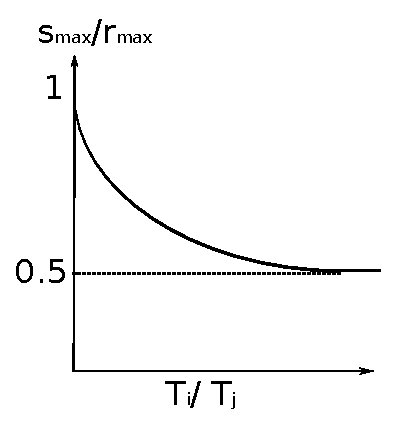
\includegraphics[scale=0.5]{figures/figure14}
\par\end{centering}

\caption{\label{fig14}Effect of $\lceil\frac{t(T_{i})}{t(T_{j})}\rceil$ on
$\frac{s_{max}}{r_{max}}$}


\end{figure}



\subsubsection{\label{sub:G-RMA-scheduler-with}G-RMA scheduler with RMA CM against
lock-free}

Equation (\ref{eq20}) is upper bounded by (\ref{eq34}) 
\begin{equation}
\sum_{(T_{j}\in\gamma_{i})\wedge(p(T_{j})\ge p(T_{i}))}(\lceil\frac{t(T_{i})-c_{j}}{t(T_{j})}\rceil+1).2.\beta_{i,j}.s_{max}\label{eq34}
\end{equation}
by considering the same assumptions as in sec \ref{sub:G-EDF-scheduler-with},
and using subscripts $k,\, l$ instead of $i,\, j$ for tasks in (\ref{eq34})
as it will be needed to discriminate between them, then the ratio
$s_{max}/r_{max}$ will be
\begin{equation}
\frac{s_{max}}{r_{max}}\le\frac{\sum_{T_{i}}(\sum_{T_{j}\in\gamma_{i}}(\lceil\frac{t(T_{i})}{t(T_{j})}\rceil+1).\beta_{i,j})/t(T_{i})}{\sum_{T_{k}}(\sum_{(T_{l}\in\gamma_{k})\wedge(p(T_{l})\ge p(T_{k}))}(\lceil\frac{t(T_{k})-c_{l}}{t(T_{l})}\rceil+1).2.\beta_{kl})/t(T_{k})}\label{eq35}
\end{equation}
The main difference between the RMA CM and the lock free is that the
former is affected only by the higher priority tasks, while the latter
is affected by all tasks (just as in G-EDF wiht EDF CM), but RMA CM
is still affected by $2.\beta_{i,j}$ (just as in G-EDF with EDF CM).
The subtraction of $c_{j}$ in the numerator in \ref{eq34} may not
have a great effect on the ratio of \ref{eq35} as the loop retrial
cost can also be modified to account for the effect of the first interfering
instance of $T_{j}$ and (\ref{eq35}) can be
\begin{equation}
\frac{s_{max}}{r_{max}}\le\frac{\sum_{T_{i}}(\sum_{T_{j}\in\gamma_{i}}(\lceil\frac{t(T_{i})-c_{j}}{t(T_{j})}\rceil+1).\beta_{i,j})/t(T_{i})}{\sum_{T_{k}}(\sum_{(T_{l}\in\gamma_{k})\wedge(p(T_{l})\ge p(T_{k}))}(\lceil\frac{t(T_{k})-c_{l}}{t(T_{l})}\rceil+1).2.\beta_{kl})/t(T_{k})}\label{eq43}
\end{equation}
If tasks in both numerator and denominator are arranged in non-increasing
order of priority, so that $i=k$, $j=l$ $\therefore$

\begin{eqnarray}
\frac{s_{max}}{r_{max}} & \le & \frac{\sum_{T_{i}}(\sum_{(T_{j}\in\gamma_{i})\wedge(p(T_{j})\ge p(T_{i}))}(\lceil\frac{t(T_{i})-c_{j}}{t(T_{j})}\rceil+1).\beta_{i,j})/t(T_{i})}{2.\sum_{T_{k}}(\sum_{(T_{l}\in\gamma_{k})\wedge(p(T_{l})\ge p(T_{k}))}(\lceil\frac{t(T_{k})-c_{l}}{t(T_{l})}\rceil+1).\beta_{kl})/t(T_{k})}+\frac{\sum_{T_{i}}(\sum_{(T_{j}\in\gamma_{i})\wedge(p(T_{j})<p(T_{i}))}(\lceil\frac{t(T_{i})-c_{j}}{t(T_{j})}\rceil+1).\beta_{i,j})/t(T_{i})}{2.\sum_{T_{k}}(\sum_{(T_{l}\in\gamma_{k})\wedge(p(T_{l})\ge p(T_{k}))}(\lceil\frac{t(T_{k})-c_{l}}{t(T_{l})}\rceil+1).\beta_{kl})/t(T_{k})}\nonumber \\
 & = & \frac{1}{2}+\frac{\sum_{T_{i}}(\sum_{(T_{j}\in\gamma_{i})\wedge(p(T_{j})<p(T_{i}))}(\lceil\frac{t(T_{i})-c_{j}}{t(T_{j})}\rceil+1).\beta_{i,j})/t(T_{i})}{2.\sum_{T_{k}}(\sum_{(T_{l}\in\gamma_{k})\wedge(p(T_{l})\ge p(T_{k}))}(\lceil\frac{t(T_{k})-c_{l}}{t(T_{l})}\rceil+1).\beta_{kl})/t(T_{k})}\label{eq36}
\end{eqnarray}
Let $\zeta_{1}=\sum_{T_{i}}(\sum_{(T_{j}\in\gamma_{i})\wedge(p(T_{j})<p(T_{i}))}(\lceil\frac{t(T_{i})-c_{j}}{t(T_{j})}\rceil+1).\beta_{i,j})/t(T_{i})$
and $\zeta_{2}=\sum_{T_{k}}(\sum_{(T_{l}\in\gamma_{k})\wedge(p(T_{l})\ge p(T_{k}))}(\lceil\frac{t(T_{k})-c_{l}}{t(T_{l})}\rceil+1).\beta_{kl})/t(T_{k})$.
But, $T_{j}$ is of lower priority than $T_{i}$, which means $D(T_{j})>D(T_{i})$
because of the G-RMA scheduler, and this means that $t(T_{j})>t(T_{i})$.
Consequently, $\lceil\frac{t(T_{i})-c_{j}}{t(T_{j})}\rceil=1$ for
all $T_{j}$ and $\zeta_{1}=\sum_{T_{i}}(\sum_{(T_{j}\in\gamma_{i})\wedge(p(T_{j})<p(T_{i}))}(2.\beta_{i,j}))/t(T_{i})$,
and (\ref{eq36}) will be 
\begin{equation}
\frac{s_{max}}{r_{max}}\le\frac{1}{2}+\frac{\sum_{T_{i}}(\sum_{(T_{j}\in\gamma_{i})\wedge(p(T_{j})<p(T_{i}))}(2.\beta_{i,j}))/t(T_{i})}{2.\sum_{T_{k}}(\sum_{(T_{l}\in\gamma_{k})\wedge(p(T_{l})\ge p(T_{k}))}(\lceil\frac{t(T_{k})-c_{l}}{t(T_{l})}\rceil+1).\beta_{kl})/t(T_{k})}\label{eq44}
\end{equation}


$\because$ $\zeta_{1}$ contains all $T_{j}$ of lower priority than
$T_{i}$, and $\zeta_{2}$ contains all $T_{l}$ of higher or equal
priority to $T_{k}$, and tasks are arranged in non-increasing order
of priority, then for each $T_{i,j}$, there exists $T_{k,l}$ such
that $i=l$ and $j=k$. This can be shown in the following figure.

\begin{center}
\begin{tabular}{ccc}
$\begin{array}{cccccc}
 & j & 1 & 2 & \cdots & n\\
i\\
1 &  & 0 & 1 & \cdots & 1\\
2 &  & 0 & 0 & \ddots & \vdots\\
\vdots &  & \vdots & \vdots & \ddots & 1\\
n &  & 0 & 0 & \cdots & 0
\end{array}$ &  & $\begin{array}{cccccc}
 & l & 1 & 2 & \cdots & n\\
k\\
1 &  & 0 & 0 & \cdots & 0\\
2 &  & 1 & 0 &  & \vdots\\
\vdots &  & \vdots & \ddots & \ddots & 0\\
n &  & 1 & \cdots & 1 & 0
\end{array}$\tabularnewline
\end{tabular}
\par\end{center}

where 0 means {}``This pair of $i,j$ does not exist in $\zeta_{1}$,
and this pair of $k,l$ does not exist in $\zeta_{2}$'', and 1 is
the reverse. So, it can be seen that both matrices are transpose of
each other, consequently, for each $\beta_{i,j}$ there exist $\beta_{k,l}$
such that $i=l$ and $j=k$, but the number of times $T_{j}$ accesses
a shared object with $T_{i}$ may not be the same as number of times
$T_{i}$ accesses that same object, so $\beta_{i,j}$ does not have
to be the same as $\beta_{k,l}$, even if $i,j$ and $k,l$ are transpose
of each other. So, we can analize behavior of $s_{max}/r_{max}$ depending
on the three parameters $\beta_{i,j}$, $\beta_{k,l}$ and $\lceil\frac{t(T_{k})-c_{l}}{t(T_{l})}\rceil$.

If $\beta_{i,j}$ is increased so that $\beta_{i,j}\rightarrow\infty$,
$\therefore\,(\ref{eq44})\rightarrow\infty$, and this is natureal
as $\beta_{i,j}$ represents times lower priority tasks $T_{j}$ access
shared objects with the higher priority task $T_{i}$. While this
number has a great effect in lock-free, it does not have any effect
in RMA CM because lower priority tasks does not affect higher priority
ones, so $s_{max}$ is allowed to be much greater than $r_{max}$.

Although the minimum value for $\beta_{i,j}$ is 1, but from a mathematical
point if $\beta_{i,j}\rightarrow0$, then $(\ref{eq44})\rightarrow1/2$.
Despite changing $\beta_{i,j}$ does not affect retrial cost of RMA
CM as lower priority tasks does not affect higher ones, but it does
affect retrial cost of lock-free bacause contention between tasks
will be reduced, thus $s_{max}$ had to be reduced in this case to
a little more than half of $r_{max}$(it is {}``a little more''
because the minimum value of $\beta_{i,j}$ is actually 1 not 0).
The change of $s_{max}/r_{max}$ is shown in Figure \ref{fig15-a}.

If $\beta_{k,l}\rightarrow\infty\,\therefore\,(\ref{eq44})\rightarrow1/2$.
This can be explained as $\beta_{k,l}$ represent number of times
a higher priority task $T_{l}$ accesses shared objects with a lower
prirority one $T_{k}$. In case of RMA CM, this will increase retrial
cost, thus reducing $s_{max}/r_{max}$. But if $\beta_{k,l}\rightarrow0,\,\therefore\,(\ref{eq44})\rightarrow\infty$,
which is explained by lower contention from higher priority task $T_{l}$
to the lower priority one $T_{k}$, consequently reduces retrial cost
in case of RMA CM and allows $s_{max}$ to be very large compared
with $r_{max}$. Of course, the actual minimum value for $\beta_{k,l}$
is 1, but this is done for mathematical illustration which is shown
in Figure \ref{fig15-b}.

The third parameter that can affect $s_{max}/r_{max}$ is the $t(T_{k})/t(T_{l})$.
If $t(T_{l})\ll t(T_{k}),\,\therefore\,\lceil\frac{t(T_{k})-c_{l}}{t(T_{l})}\rceil\rightarrow\infty$,
and $(\ref{eq44})\rightarrow1/2$. This is explained by a high number
of interferences of higher priority tasks $T_{l}$ to a lower priority
one $T_{k}$ that increases retrial cost in case of RMA CM, consequently,
reduces $s_{max}/r_{max}$. But if $t(T_{l})=t(T_{k})$ (which is
the maximum value for $t(T_{l})$ as $D(T_{l})\le D(T_{k})$ because
$T_{l}$ is of higher or equal priority to $T_{k}$), $\therefore\,\lceil\frac{t(T_{k})-c_{l}}{t(T_{l})}\rceil\rightarrow1$
and the right side of $([eq44])\rightarrow\frac{1}{2}+\frac{\sum_{T_{i}}(\sum_{(T_{j}\in\gamma_{i})\wedge(p(T_{j})<p(T_{i}))}(2.\beta_{i,j}))/t(T_{i})}{2.\sum_{T_{k}}(\sum_{(T_{l}\in\gamma_{k})\wedge(p(T_{l})\ge p(T_{k}))}(2.\beta_{kl}))/t(T_{k})}$
which renders the system one of the two previous cases shown in Figures
\ref{fig15-a},\ref{fig15-b}.

\begin{center}
\begin{figure}
\begin{centering}
\subfloat[\label{fig15-a}(a)]{\begin{centering}
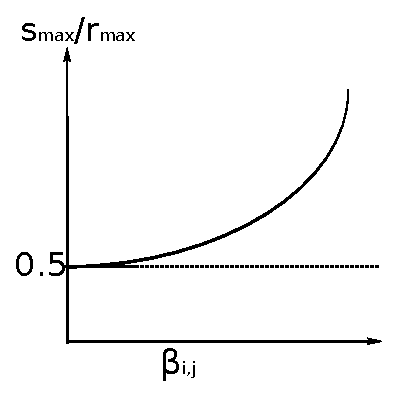
\includegraphics[scale=0.5]{figures/figure15-a}
\par\end{centering}

}\subfloat[\label{fig15-b}(b)]{\begin{centering}
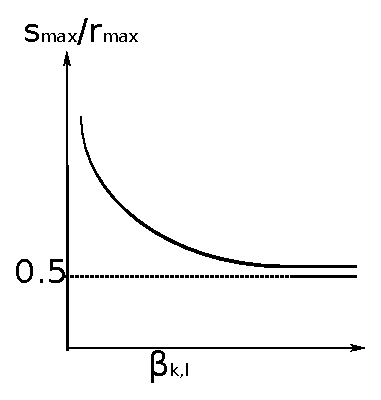
\includegraphics[scale=0.5]{figures/figure15-b}
\par\end{centering}



}
\par\end{centering}

\centering{}\caption{\label{fig15}Change of $s_{max}/r_{max}$ a) $\frac{s_{max}}{r_{max}}$
vs. $\beta_{i,j}$ b) $\frac{s_{max}}{r_{max}}$ vs. $\beta_{k,l}$
c)}
\end{figure}

\par\end{center}


\subsubsection{FIFO CM against lock-free}

For both G-EDF and G-RMA with FIFO CM, the retrial cost is the same,
and the $s_{max}/r_{max}$ will be
\begin{eqnarray}
\frac{s_{max}}{r_{max}} & \le & \frac{\sum_{T_{i}}(\sum_{T_{j}\in\gamma_{i}}((\lceil\frac{t(T_{i})-c_{j}}{t(T_{j})}\rceil+1).\beta_{i,j}))/t(T_{i})}{\sum_{T_{i}}(\sum_{T_{j}\in\gamma_{i}}((\lceil\frac{t(T_{i})-c_{j}}{t(T_{j})}\rceil+1).\beta_{i,j}))/t(T_{i})}\nonumber \\
 & \le & 1\label{eq37}
\end{eqnarray}
So, in the case of FIFO CM, $s_{max}$ is allowed to be as large as
that of $r_{max}$ without degrading performance than lock free implementation.


\subsection{\label{sub:Comparison-between-FMLP}Comparison between FMLP and G-EDF
with EDF CM and FIFO CM}

As FMLP is used with G-EDF, G-EDF with EDF CM and FIFO CM are compared
here. For the case of non-nested requests, each resource (short or
long) will be contained in its own group, and the three terms of blocking
by FMLP can be upper bounded as follows:-
\begin{eqnarray*}
BW(T_{i}) & \le & \sum_{s\_\theta\in\theta_{i}}(m-1).|s\_\theta|_{i,max}\\
 & = & N_{i,s}.(m-1).|s\_\theta|_{i,max}\\
 & \le & N_{i,s}.(m-1).|s\_\theta|_{max}
\end{eqnarray*}
where $N_{i,s}$ is the number of times $T_{i}$ requests a short
resource, and $|s\_\theta|_{i,max}$ is the maximum request for a
short resource by $T_{i}$, and $|s\_\theta|_{max}$ is the maximum
short request by any task. And 
\begin{eqnarray*}
NPB(T_{i}) & \le & (1+N_{i,l}).max(BW_{k\ne i}(T_{k})+|s\_\theta|_{k,max})\\
 & \le & (1+N_{i,l}).max(BW_{k\ne i}(T_{k})+|s\_\theta|_{max})\\
 & = & (1+N_{i,l}).|s\_\theta|_{max}.max_{k\ne i}(N_{k,s}.(m-1)+1)
\end{eqnarray*}
and
\begin{eqnarray*}
DB(T_{i}) & \le & N_{i,l}.(n-1).|l\_\theta|_{i,max}\\
 & \le & N_{i,l}.(n-1).|l\_\theta|_{max}
\end{eqnarray*}
if $|l\_\theta|_{max}\le c1.|s\_\theta|_{max}$ where $c1$ is the
minimum constant that satisfies this relation, then
\[
DB(T_{i})\le N_{i,l}.(n-1).c1.|s\_\theta|_{max}
\]
The total blocking of each task is added to its execution time, and
as before, the total utilization of G-EDF system (with both contention
managers) is compared to that of FMLP. For performance of G-EDF with
EDF CM to be better than FMLP, then
\begin{eqnarray*}
s_{max}\sum_{T_{i}}(\sum_{T_{j}\in\gamma_{i}}\lceil\frac{t(T_{i})}{t(T_{j})}\rceil.2\beta_{i,j})/t(T_{i}) & \le|s\_\theta|_{max}\sum_{T_{i}}[( & N_{i,s}.(m-1)+\\
 & + & (1+N_{i,l}).max_{k\ne i}(N_{k,s}.(m-1)+1)\\
 & + & N_{i,l}.(n-1).c1)]/t(T_{i})
\end{eqnarray*}
$\therefore$
\begin{equation}
\frac{s_{max}}{|s\_\theta|_{max}}\le\frac{\sum_{T_{i}}[(N_{i,s}.(m-1)+(1+N_{i,l}).max_{k\ne i}(N_{k,s}.(m-1)+1)+N_{i,l}.(n-1).c1)]/t(T_{i})}{\sum_{T_{i}}(\sum_{T_{j}\in\gamma_{i}}\lceil\frac{t(T_{i})}{t(T_{j})}\rceil.2\beta_{i,j})/t(T_{i})}\label{eq38}
\end{equation}
and for G-EDF with FIFO CM, this ratio will be
\begin{equation}
\frac{s_{max}}{|s\_\theta|_{max}}\le\frac{\sum_{T_{i}}[(N_{i,s}.(m-1)+(1+N_{i,l}).max_{k\ne i}(N_{k,s}.(m-1)+1)+N_{i,l}.(n-1).c1)]/t(T_{i})}{\sum_{T_{i}}(\sum_{T_{j}\in\gamma_{i}}((\lceil\frac{t(T_{i})-c_{j}}{t(T_{j})}\rceil+1).\beta_{i,j}))/t(T_{i})}\label{eq39}
\end{equation}


From (\ref{eq38}) and (\ref{eq39}), it can be seen that $T_{i}$,
in FMLP, depends on $m,\, n$ and number of times it requests resources
(in contrast to G-EDF with EDF or FIFO CM, which depends on number
of times the conflicting $T_{j}$ requests resources). So, if $N_{i,s},\, N_{i,l}$
and $N_{k,s}$ can all be upper bounded by some constant $C_{2}$,
which is the maximum number of times any $T_{i}$ can ask for a short
or long resource, then the numerator in (\ref{eq38}) and (\ref{eq39})
is $O(n(n+m))$, while the denominator is $O(n^{2})$. So, 
\begin{equation}
\frac{s_{max}}{|s\_\theta|_{max}}=O(\frac{m}{n})\label{eq45}
\end{equation}
which means, for $n<m$, contention between tasks in both STM and
FMLP is low (even for short resources in FMLP), but FMLP is more affected
by $NTB$. But when $n>m$, contention increases, but FMLP arranges
requests in a FIFO queue, so it is leass affected than EDF CM which
sufferes from number of conflicting tasks and number of instances
of each conflicting one. FMLP is not affected by number of instances
of each conflicting task, and FIFO CM, although arranging requests
in a FIFO order, but this order can change due to release in higher
priority tasks as previously discussed in \ref{sec:Response-time-of FIFO CM},
so FIFO CM is also affected by number of instances of conflicting
tasks.


\section{\label{sec:Comparison-of-OMLP}Comparison of OMLP with STM}

As blocking time for OMLP is bounded by
\[
b_{i}\triangleq\sum_{k=1}^{q}N_{i,k}.2.(m-1).max_{1\le i\le n}\{L_{i,k}\}
\]
where $N_{i,k}$ is the maximum number of times $T_{i}$ requests
resource $k$, and $L_{i,k}$ is the maximum length of such a request.
So, if $L_{max}=max_{\forall i,\forall k}L_{i,k}$, $\therefore$
\[
bi\le2.(m-1).L_{max}\sum_{k=1}^{q}N_{i,k}
\]
and for performance of G-EDF with EDF CM to be better than global
OMLP, then
\begin{equation}
\frac{s_{max}}{L_{max}}\le\frac{\sum_{T_{i}}(2.(m-1)\sum_{k=1}^{q}N_{i,k})/t(T_{i})}{\sum_{T_{i}}(\sum_{T_{j}\in\gamma_{i}}\lceil\frac{t(T_{i})}{t(T_{j})}\rceil.2\beta_{i,j})/t(T_{i})}\label{eq40}
\end{equation}
For G-RMA with RMA CM, the ratio will be
\begin{equation}
\frac{s_{max}}{L_{max}}\le\frac{\sum_{T_{i}}(2.(m-1)\sum_{k=1}^{q}N_{i,k})/t(T_{i})}{\sum_{T_{i}}(\sum_{(T_{j}\in\gamma_{i})\wedge(p(T_{j})\ge p(T_{i}))}(\lceil\frac{t(T_{i})-c_{j}}{t(T_{j})}\rceil+1).2.\beta_{i,j})/t(T_{i})}\label{eq41}
\end{equation}
and for FIFO CM for both G-EDF and G-RMA schedulers
\begin{equation}
\frac{s_{max}}{L_{max}}\le\frac{\sum_{T_{i}}(2.(m-1)\sum_{k=1}^{q}N_{i,k})/t(T_{i})}{\sum_{T_{i}}(\sum_{T_{j}\in\gamma_{i}}((\lceil\frac{t(T_{i})-c_{j}}{t(T_{j})}\rceil+1).\beta_{i,j}))/t(T_{i})}\label{eq42}
\end{equation}


If $\sum_{k=1}^{q}N_{i,k}$ is upper bounded by $C_{3}$, which is
a constant representing the maximum total number of requests for resources
by any $T_{i}$, then 
\begin{equation}
\frac{s_{max}}{L_{max}}=O(\frac{nm}{n^{2}})=O(\frac{m}{n})\label{eq46}
\end{equation}
for each of (\ref{eq40}), (\ref{eq41}) and (\ref{eq42}) which is
similar to that of FMLP.


\subsection{Conclusion on comparison between synchronization techniques}

Comparison between STM, with the three contention managers, against
lock-free is somehow different than that between STM and locking protocols
in that the former have similar parameters that affect retrial cost
of both STM and lock-free (i. e.; number of conflicting tasks, number
of instances of these conflicting tasks, number of shared objects
and number of their requests by conflicting tasks). So, $T_{i}$ is
mostly affected by the nature of other tasks. But blocking time in
FMLP and OMLP depend on some different parameters than that in STM
and lock-free, as requests are arranged in a queue, and the order
of the request in the queue does not change (except for the case of
the priority queue in OMLP), so blocking time depend on number of
tasks but not on number of instances of conflicting tasks, and it
depends on number of requests made by $T_{i}$ itself, and not the
coflicting tasks; it also depends on number of processors in both
protocols, which is not the case in STM and lock-free. That is why
comparison between STM and locking protocols has the asymptotic nature,
while in STM and lock-free, effect of different parameters can be
compared together.

For the comparison between STM and lock-free, it has been seen that
both EDF and RMA CM suffer from $2.s_{max}$ retrial cost for each
atomic section of $T_{i}$ by one atomic section of $T_{j}$, while
FIFO CM does not. Retrial in RMA, FIFO CM and lock-free is affected
by a larger number of conflicting instances than that of EDF CM, while
EDF, FIFO CM and lock-free can be affected by all other tasks, but
RMA CM is affected only by higher priority tasks. Due to the different
parameters affecting STM and lock-free, the $s_{max}/r_{max}$ differs
to keep STM better or good as lock-free. In G-EDF with EDF CM, this
ratio cannot exceed 1 and it can be kept at one half for higher number
of conflicting tasks. For, G-RMA with RMA CM, it differs according
to different parameters, but $s_{max}$ can be larger than $r_{max}$
by many times at some cases, but the common case to keep STM performance
well, is to keep it at one half of $r_{max}$. For the FIFO CM, $s_{max}$
can be as large as $r_{max}$, so it increased the minimum bound for
$s_{max}/r_{max}$ over that of EDF and RMA CM, but RMA can have a
larger $s_{max}$ in some cases.

So, it appears that each method has its merits and disadvantages.
It is up to the designer to choose according to the parameters values
of its application, in addition to noting the simplisity of STM programability,
in contrast to that of lock-free approache.

\newpage{}


\section{Further improvements to ECM and RCM: multi-object transactions and
reducing retry cost}


\subsection{Probelm Description\label{probelm description}}

Previous analysis is suitable only for transactions that share one
object, but this is not suitable for reality. Some reasons that make
the analysis for multi-object transactions difficult can be illustrated
by the following example.

\textbf{Example 1:} Assume three atomic sections $s_{1}^{x}$, $s_{2}^{y}$
and $s_{3}^{z}$ belonging to jobs $\tau_{1}^{x}$,$\tau_{2}^{y}$
and $\tau_{3}^{z}$, with priorities $p_{1}^{x}>p_{2}^{y}>p_{3}^{z}$.
$s_{1}^{x}$ and $s_{2}^{y}$ share objects, $s_{2}^{y}$ and $s_{3}^{z}$
share objects, but $s_{1}^{x}$ and $s_{3}^{z}$ do not share objects.
$s_{1}^{x}$ can make $s_{2}^{y}$ to retry which in turn will make
$s_{3}^{z}$ to retry, this means that $s_{3}^{z}$ is retrying transitively
because of $s_{1}^{x}$, which will increase retry cost of $s_{3}^{z}$.
Problem gets more complicated if another atomic section $s_{4}^{f}$,
belonging to $\tau_{4}^{f}$ where $p_{4}^{f}>p_{1}^{x}$, shares
objects with $s_{1}^{x}$, but shares nothing with $s_{2}^{y}$ nor
$s_{3}^{z}$. Thus, transitive retry will move from $s_{4}^{f}$ to
$s_{3}^{z}$, increasing the retry cost of $s_{3}^{z}$. The situation
gets worse as more tasks of higer priority are added where each task
shares objects with its immediate lower priority task. $\tau_{1}^{x}$
may have atomic sections that share objects with $\tau_{3}^{z}$,
but this will not prevent the effect of transitive retry due to $s_{1}^{x}$.

\begin{mydef}

\textbf{Transitive Retry:} A transaction $s_{i}^{k}$ suffers from
transitive retry when it conflicts with a higer priority transaction
$s_{j}^{l}$, which in turn conflicts with a higher priority transaction
$s_{z}^{h}$, but $s_{i}^{k}$ does not conflict with $s_{z}^{h}$.
Still, when $s_{j}^{l}$ retries due to $s_{z}^{h}$, $s_{i}^{k}$
also retries due to $s_{j}^{l}$. Thus, the effect of the higher priority
transaction $s_{z}^{h}$ is transitively moved to the lower priority
transaction $s_{i}^{k}$, despite they do not conflict on common objects.

\end{mydef}

\begin{clm}\label{ecm-rcm-transitive-retry}

ECM and RCM suffer from transitive retry for multi-object transactions.

\end{clm}

\begin{proof}

Example 1, mentioned previously, applies under both ECM and RCM where
priority for each transaction in ECM is defined as its containing
job absolute deadline, and in RCM, transaction priority is the period
of the containg task. Claim follows. 

\end{proof}

So, what is needed here is to extend the set of objects that can make
an atomic section of lower priority job to retry. This can be done
by initializing the set of conflicting object to all objects accessed
by all transactions in the analyzed task, then looping through all
transactions belonging to all other higher priority tasks, and each
trasnaction that accesses at least one of the objects in the set of
conflicting objects is going to add all other objects accessed by
this transaction to the set. This loop over all higher priority tasks
is repeated again and again, each time with the new set of objects
until there is no more transactions accessing any object in the set.
As it seems, this solution can extend the set of conflicting objects
too much, and may even contain all objects access by all tasks.

So, what is provided here is a new contention manager that avoids
the effect of transitive retry. This contention manager is called
Priority Contention Manager with Negative values and First access
(PCM-N-F) and is described in Section \ref{pcm-n-f}. For convenince,
terms {}``atomic section'' and {}``transaction'' are used interchangably,
and the priority of a transaction is the priority of the enclosing
job.


\subsection{\label{pcm-n-f}Priority Contention Manager with Negative values
and First Access (PCM-N-F)}

\begin{algorithm}
\footnotesize{
\linesnumbered
\KwData{
Executing Transaction: is one that cannot be aborted by any other transaction, nor preempted by a higer priority task\;
m\_set: m-length set that contains only non-conflicting exececuting transactions\;
n\_set: n-length set that contains retrying transactions for n tasks in non-increasing order of priority\;
n(z): transaction at index z of the n\_set\;
$s_i^k$: a new released transaction\;
$s_j^l$: one of the executing transactions\;
}
\KwResult{which atomic section(s) is(are) going to commit}
\eIf{$s_i^k$ does not conflict with any executing transaction\label{s_i^k true}}
{
Assign $s_i^k$ as an executing transaction\;
Add $s_i^k$ to the m\_set\;
$s_i^k$ is to commit
}
{
Add $s_i^k$ to the n\_set according to its priority\label{move to n}\;
Assign temporal priority to job that owns $s_i^k$ to -1\label{priority to -1}\;
The conflicting executing transaction(s) with $s_i^k$ is(are) the one(s) to commit\label{s_i^k commit}\;
}
\If{$s_j^l$ commits\label{s_j^l commits}}
{
	\For{z=1 to size of n\_set\label{traverse n_set}}
	{
		\If{n(z) does not conflict with any executing transaction\label{n(z) no conflict}}
		{
			\If{processor available\label{processor available}}
			{
				Restore priority of task owning n(z)\;
				Assign n(z) as executing transaction\;
				Add n(z) to m\_set\;
				n(z) to commit\;
			}
		}
		move to the next n(z)\;
	}
}
}
\caption{PCM-N-F} \label{PCM-N-F-algorithm}
\end{algorithm}

PCM-N-F works as defined in Algorithm \ref{PCM-N-F-algorithm}. It
manages two sets: the {}``m\_set'' which contains at most m non-conflicting
transactions, where m is the number of processors in the system, as
there cannot be more than m executing transactions (or generally,
m executing jobs) the the same time. When a transaction is entered
in the {}``m-set'', it executes non-preemptively and no other transaction
can abort it. Any transaction in the {}``m-set'' is called {}``Executing
Transaction''. This means when a transaction is executing before
the arrival of higher priority conflicting transactions, then the
one that started executing first is the one to commit (Step~\ref{s_i^k commit}),
hence the term {}``First'' is in the name of the algorithm.

The other set is the {}``n-set'' which holds the the transactions
that are retrying because of conflict with one or more of the {}``Executing
Transactions'' (Step~\ref{move to n}), and {}``n'' stands for
the number of tasks in the system. It also holds transactions that
cannot execute currently because processors are busy, either by processing
{}``Executing Transactions'' and/or by processing higher priority
jobs. Any transaction in the {}``n-set'' is assigned a temporal
priority of {}``-1'' (Step~\ref{priority to -1}), hence the term
{}``Negative'' in the name of the algorithm. {}``Negative'' priority
is considered smaller than any normal priority, and a transaction
continues to hold this negative priority until it is moved to the
{}``m-set'' where it restores its normal priority. The {}``n-set''
can hold transactions that had been preempted by higher prirority
jobs, even if these higher priority jobs do not have transactions
to conflict with those preempted transactions, hence this set is of
length {}``n'' as there can be at most n jobs in the system at the
same time. This list keeps track even of preempted transactions, because
as it will be shown, these transactions are examined when any of the
executing transaction commits, and any of these transactions can restore
its original priority which can be higher than the preempting job,
thus the aborted transaction can preempt the job which previously
preempted it when the transaction was in the {}``n\_set''.

When a new transaction is released, and it does not conflict with
any one of the executing transactions (Step~\ref{s_i^k true}), then
it is going to allocate a slot in the {}``m\_set'' and become an
{}``executing transaction'' itself. As this transaction is released,
this means that its owning task is already allocated to processor,
so this new transaction does not face the problem of unavailable processors.
This new transaction might have a conflict with any of the transactions
in the {}``n\_set'', but as transactions in the {}``n\_set'' have
priorities of -1, so they cannot prevent this new transaction from
executing if does not conflict with any of the executing transactions.

When one of the executing transactions commits (Step~\ref{s_j^l commits}),
then it is time to select one of the {}``n\_set'' transactions to
commit. The {}``n\_set'' is traversed from the highest priority
transaction to the lower priority (where priority here refers to the
original priority of the transactions, not the -1) (Step~\ref{traverse n_set}),
and if the examined transaction in the {}``n\_set'', $s_{h}^{b}$,
does not conflict with any executing transaction (Step~\ref{n(z) no conflict}),
and there is an available processor for it (Step~\ref{processor available})
(where {}``available'' means either an idle processor, or one that
is executing a job of lower priority than that of the examined transaction),
then this examined transaction in the {}``n\_set'' is moved to the
{}``m\_set'' where it becomes an {}``executing transaction'' and
restores its original prirority. If $s_{h}^{b}$ is added to the {}``m\_set'',
the new {}``m\_set'' is used in comparison against other transactions
in the {}``n\_set'' with lower priority than $s_{h}^{b}$. So, if
one of the transactions in the {}``n\_set'', $s_{d}^{g}$, is of
lower priority than $s_{h}^{b}$ and is conflicting with $s_{h}^{b}$,
it will remain in the {}``n\_set''. So, the choice of the new transaction
from the {}``n\_set'' depends on original priority of transactions,
hence the term {}``PCM'' in the name of the algorithm. So, the algorithm
avoids inturrpting an already executing transaction to reduce its
retry cost, meanwhile, it tries to avoid delaying the higest priority
transaction in the {}``n\_set'' when it is time to select a new
one to commit, even if this highest priority transaction arrives after
other lower priority transactions in the {}``n\_set''.


\subsection{PCM-N-F properties}

\begin{clm}\label{pcm-n-f-transitive-retry}

Transactions scheduled under PCM-N-F do not suffer from transitive
retry.

\end{clm}

\begin{proof}

Proof is done by contradiction. Assuming a transaction $s_{i}^{k}$
is retrying because of higher priority transaction $s_{j}^{l}$ which
in turn is retrying because of another higher priority transaction
$s_{z}^{h}$, but $s_{i}^{k}$ and $s_{z}^{h}$ do not conflict, yet,
$s_{i}^{k}$ is transitively retrying because of $s_{z}^{h}$. It
is noted that $s_{z}^{h}$ and $s_{j}^{l}$ cannot exit together in
the {}``m\_set'' as they have common objects, but they both can
exist in the {}``n\_set'' as they both can conflict with other executing
transactions. So, we have three cases:

\textit{Case 1:} assuming $s_{z}^{h}$ is an executing transaction,
this means that $s_{j}^{l}$ is in the {}``n\_set'' and when $s_{i}^{k}$
arrives, by definition of PCM-N-F, it will be compared against the
{}``m\_set'', which contains $s_{z}^{h}$, and it will be found
that $s_{i}^{k}$ does not conflict with $s_{z}^{h}$. Also, by definition
of PCM-N-F, $s_{i}^{k}$ is not compared aginst transactions in the
{}``n\_set'' when it newly arrives, as priorities of {}``n\_set''
transaction is lower than any normal priority. So, if there are available
processors and $s_{i}^{k}$ does not conflict with any other executing
transaction, it joins the {}``m\_set'' and becomes an {}``executing
transaction'' which contradicts the assumption that $s_{i}^{k}$
is transitively retrying because of $s_{z}^{h}$.

\textit{Case 2:} $s_{z}^{h}$ is in the {}``n\_set'', while $s_{j}^{l}$
is an executing transaction. When $s_{i}^{k}$ arrives, it will conflict
with $s_{j}^{l}$ and joins the {}``n\_set''. Now, $s_{i}^{k}$
retries due to $s_{j}^{l}$, not $s_{z}^{h}$. When $s_{j}^{l}$ commits,
the {}``n\_set'' is traversed from the highest priority transaction
to the lowest one; if $s_{z}^{h}$ does not conflict with any other
executing transaction and there are available processors, $s_{z}^{h}$
becomes an executing transaction. When $s_{i}^{k}$ is compared against
the {}``m\_set'', it is found that it does not conflict with $s_{z}^{h}$,
and if it also does not conflict with any other executing transaction
and there are available processors, $s_{i}^{k}$ becomes and executing
transaction, which means $s_{i}^{k}$ and $s_{z}^{h}$ are executing
concurrently. This also violates the assumption of transitive retrying.

\textit{Case 3:} $s_{z}^{h}$ and $s_{j}^{l}$ both exist in the {}``n\_set''.
When $s_{i}^{k}$ arrives and comared against the {}``m\_set'',
it can become an executing transaction if it does not conflict with
any executing one and there available processors. Despite $s_{i}^{k}$
have common objects with $s_{j}^{l}$, but $s_{i}^{k}$ is not compared
aginst $s_{j}^{l}$ which is in the {}``n\_set''. If $s_{i}^{k}$
is going to join the {}``n\_set'', this is done because it conflicts
with one or more executing transactions or due to lack of processors,
not because of $s_{z}^{h}$ which violates the transitive retry assumption.

If the three transactions exist in the {}``n\_set'' and it is time
to choose the new executing transactions. If $s_{z}^{h}$ is chosen,
then $s_{j}^{l}$ remains in the {}``n\_set'' and this leads to
Case 1, but if $s_{j}^{l}$ is chosen, because $s_{z}^{h}$ conflicts
with another executing transaction but $s_{j}^{l}$ does not, then
this leads to Case 2. Claim follows.

\end{proof}

\begin{clm}\label{first-access}

{}``First access'' property ({}``F'' term in PCM-N-F) is important
to avoid increased retry cost of transactions suffering from transitive
retry.

\end{clm}

\begin{proof}

Proof is done by contradiction. Assuming retry cost of transactions
in the absence of {}``First access'' property is the same when {}``First
access'' exists. Then, {}``First access'' is assumed to not apply
to PCM-N-F, and executing transactions can be aborted. Assuming only
three transactions $s_{i}^{k}$, $s_{j}^{l}$ and $s_{z}^{h}$, where
priority of $s_{z}^{h}$ is higher than priority of $s_{j}^{l}$,
which in turn has a higher priority than that of $s_{i}^{k}$. Assuming
$s_{j}^{l}$ conflicts with both $s_{i}^{k}$ and $s_{z}^{h}$, but
$s_{i}^{k}$ and $s_{z}^{h}$ do not conflict together. If $s_{i}^{k}$
arrives when $s_{z}^{h}$ is an executing transaction and $s_{j}^{l}$
is in the {}``n\_set'', then $s_{i}^{k}$ can be an executing transaction
itself while $s_{j}^{l}$ is retrying. But if $s_{i}^{k}$ did not
commit at least when $s_{z}^{h}$ commit, then $s_{j}^{l}$ can become
an executing transaction, and because of lack of {}``First access''
property, $s_{j}^{l}$ will enforce $s_{i}^{k}$ to retry. So, the
retry cost for $s_{i}^{k}$ will be $len(s_{z}^{h}+s_{j}^{l})$, which
is the same retry cost for $s_{i}^{k}$ if it had been transitively
retrying because of $s_{z}^{h}$ which contradicts with the first
assumption. Claim follows.

\end{proof}

\begin{clm}

PCM-N-F handles multi-object transactions better than ECM and RCM.

\end{clm}

\begin{proof}

From Claims \ref{ecm-rcm-transitive-retry}, \ref{pcm-n-f-transitive-retry}
and \ref{first-access}, it appears that PCM-N-F does not increase
retry cost of multi-object transactions, in contrast to what is done
under ECM and RCM. Claim follows.

\end{proof}

\begin{clm}\label{higher retry does not affect response}

Any job $\tau_{i}^{x}$ is not affected by retry cost in any other
job $\tau_{j}^{l}$.

\end{clm}

\begin{proof}

Because of the behavior of PCM-N-F, any retrying transaction is assigned
a temportal priority of -1, which is lower than any other priority.
So, when $\tau_{i}^{x}$ is released, it will have a higher priority
than any higher or lower priority job $\tau_{j}^{l}$ with temporal
priority of -1.

\end{proof}


\subsection{Retry Cost under PCM-N-F}

To determine an upper bound for transactions under PCM-N-F, the following
Claims are introduced.

\begin{clm}\label{two transactions retry cost pcm-n-f}

Assuming only two conflicting transactions $s_{i}^{k}$ and $s_{j}^{l}$.
Under PCM-N-F, the maximum retry cost suffered by $s_{i}^{k}$ due
to $s_{j}^{l}$ is $len(s_{j}^{l})$.

\end{clm}

\begin{proof}

By definition of PCM-N-F, $s_{i}^{k}$ cannot have started before
$s_{j}^{l}$, otherwise, it would have been an executing transaction
and $s_{j}^{l}$ cannot abort it, whether $s_{j}^{l}$ is of higher
or lower priority than $s_{i}^{k}$. So, at most, $s_{i}^{k}$ have
started just after $s_{j}^{l}$, and it has to wait until $s_{j}^{l}$
commits, so $s_{i}^{k}$ can start. Claim follows.

\end{proof}

\begin{clm}

The retry cost for any job $\tau_{i}^{k}$ during an interval $L\le T_{i}$
due to conflict between its transactions and transactions of other
jobs under PCM-N-F is upper bounded by 
\begin{equation}
RC(L)\le\sum_{\tau_{j}\in\gamma_{i}}\left(\sum_{\theta\in\theta_{i}}\left(\left(\left\lceil \frac{L}{T_{j}}\right\rceil +1\right)\sum_{\bar{\forall s_{j}^{k}(\theta)}}len\left(\bar{s_{j}^{k}(\theta)}\right)\right)\right)\label{rc-pcm-n-f}
\end{equation}
where $\bar{s_{j}^{k}(\theta)}$ is the same as $s_{j}^{k}(\theta)$,
but if $s_{j}^{k}$ accesses more than one object $\theta\in\theta_{i}$,
then $len(s_{j}^{k})$ is included only once in the last summation
as a representative of all accessed objects by $s_{j}^{k}$. 

\end{clm}

\begin{proof}

Assuming a transaction $s_{i}^{k}$ belonging to job $\tau_{i}^{x}$.
The worst case scenario for $s_{i}^{k}$ occurs when it conflicts
with one or more executing transactions, then $s_{i}^{k}$ has to
wait in the {}``n\_set'', and all higher priority transactions conflicting
with $s_{i}^{k}$ are chosen before $s_{i}^{k}$ to be executing transaction.
When a higher priority transaction $s_{z}^{h}$, conflicting with
$s_{i}^{k}$, becomes an executing transaction, another lower priority
transaction $s_{l}^{f}$- which does not conflict with any executing
transaction- can become an executing transaction itself. Thus, $s_{i}^{k}$
can wait for both higher and lower priority conflicting transactions.
$\bar{s_{j}^{k}(\theta)}$ is used because $s_{j}^{k}$ does not repeat
itself for each object it access, in addition to the notion that the
same $s_{j}^{l}$ or $s_{l}^{f}$ cannot enforce more than one transaction
in $\tau_{i}^{x}$ to retry because if $s_{j}^{l}$, or $s_{l}^{f}$,
enforces $s_{i}^{k}$ to retry, this means that $s_{j}^{l}$, or $s_{l}^{f}$,
is an executing transaction and it will commit before the next transaction
in $\tau_{i}^{x}$ arrives. Combining this with Claim \ref{two transactions retry cost pcm-n-f}
and the maximum number of jobs of any task $\tau_{j}$ that can interfere
with $\tau_{i}^{x}$ during interval $L$ is $\left\lceil \frac{L}{T_{j}}\right\rceil +1$,
then Claim follows.

\end{proof}

\begin{clm}\label{delay}

The delay time, for a job $\tau_{i}^{x}$, due to lower priority jobs,
during an interval $L\le T_{i}$, is upper bounded by 
\begin{equation}
D(\tau_{i}^{x})\le\left\lfloor \frac{1}{m}\sum_{\forall\bar{\tau_{j}^{l}}}\left(\left(\left\lceil \frac{L}{T_{j}}\right\rceil +1\right)\sum_{\forall\bar{s_{j}^{h}}}len\left(\bar{s_{j}^{h}}\right)\right)\right\rfloor \label{pcm-n-f-delay}
\end{equation}
where $D(\tau_{i}^{x})$ is delay time suffered by $\tau_{i}^{x}$
due to lower priority jobs, $\bar{\tau_{j}^{l}=\{\tau_{j}^{l}:p_{j}^{l}<p_{i}^{x}\}}$
and $\bar{s_{j}^{h}}=\{s_{j}^{h}:s_{j}^{h}\, does\, not\, conflict\, with\, any\, s_{i}^{k}\}$.
During this delay time, all processor are unavailable for $\tau_{i}^{x}$.

\end{clm}

\begin{proof}

Lower priority jobs can delay $\tau_{i}^{x}$ only at executing transactions
of these jobs, because executing transactions are non-preemptive.
These lower priority executing transactions can be conflicting with
transactions in $\tau_{i}^{x}$, in which case, their effect is retry
cost to $\tau_{i}^{x}$ which is already included in Equation \ref{rc-pcm-n-f}.
When these lower priority transactions are non-conflicting with any
transaction in $\tau_{i}^{x}$, they act as if they were higher priority
jobs interfering with $\tau_{i}^{x}$ whose interference workload
(which is the delay they casue to $\tau_{i}^{x}$) can be calculated
by Theorem 1 in \cite{key-2}. If not all processors are busy with
these lower priority transactions, then $\tau_{i}^{x}$ can run in
parallel with them on a free processor because these lower priority
transactions are non-conflicting with any transaction in $\tau_{i}^{x}$,
but the problem appears all processors are busy with higher priority
jobs and/or lower priority non-conflicting transactions. So, during
the delay time, no processors are available for $\tau_{i}^{x}$. Claim
follows.

\end{proof}

\begin{clm}\label{response time ecm pcm-n-f}

Assuming a multiprocessor system scheduled with G-EDF and synchronization
is done by STM with PCM-N-F used as the contention manager. The response
time of a job $\tau_{i}^{x}$, during an interval $L\le T_{i}$, is
upper bounded by 
\begin{equation}
R_{i}^{up}=c_{i}+RC(L)+D_{edf}(\tau_{i}^{x})+\left\lfloor \frac{1}{m}\sum_{\forall j\ne i}W_{ij}(R_{i}^{up})\right\rfloor 
\end{equation}
where $RC(L)$ is calculated by (\ref{rc-pcm-n-f}), and $D_{edf}(\tau_{i}^{x})$
is the same as $D(\tau_{i}^{x})$, defined in Equation \ref{pcm-n-f-delay},
but for G-EDF scheduled systems, (\ref{pcm-n-f-delay}) is modified
to 
\begin{eqnarray}
D_{edf}(\tau_{i}^{x}) & \le & \left\lfloor \frac{1}{m}\sum_{\forall\bar{\tau_{j}^{l}}}\begin{cases}
0 & ,L\le T_{i}-T_{j}\\
\sum_{\forall\bar{s_{j}^{h}}}len\left(\bar{s_{j}^{h}}\right) & ,L>T_{i}-T_{j}
\end{cases}\right\rfloor \label{d-edf}
\end{eqnarray}
and $W_{ij}(R_{i}^{up})$ is calculated by Equation \ref{eq13}.

\end{clm}

\begin{proof}

Response time for $\tau_{i}^{x}$ is calculated as in Equation \ref{eq10}
except that delay time of lower priority tasks is added as defined
by Claim \ref{delay}, but as G-EDF uses absolute deadlines for scheduling,
this affects which jobs can be of lower priority than $\tau_{i}^{x}$
and which will be of higher priority as follows: During $T_{i}$,
all instance of task $\tau_{j}$ will be of higher priority than $\tau_{i}^{x}$
except the instance of $\tau_{j}$ that is released after $T_{i}-T_{j}$,
because that last instance will have a longer absolute deadline than
$\tau_{i}^{x}$. So, as our interest only in interval $L\le T_{i}$,
then there can be only one instance of each task (that is why $\left\lceil \frac{L}{T_{j}}\right\rceil +1$
in Equation \ref{pcm-n-f-delay} is replaced with 1 in the second
case in Equation \ref{d-edf}) interfering with $\tau_{i}^{x}$, that
can have a lower priority than $\tau_{i}^{x}$, and this lower priority
instance is released only if $L>T_{i}-T_{j}$ (this is why 0 is used
in the first case in (\ref{d-edf})). Claim follows.

\end{proof}

$W_{ij}(R_{i}^{up})$ is defined by Equation \ref{eq13} instead of
Equation \ref{eq10} (which is used in ECM) because- in contrast to
ECM- retry cost of higher priority jobs does not affect response time
of $\tau_{i}^{x}$ as proved in Claim \ref{higher retry does not affect response}

\begin{clm}\label{response rcm pcm-n-f}

Assuming a multiprocessor system scheduled with G-RMA and synchronization
is done by STM with PCM-N-F used as the contention manager. Response
time of job $\tau_{i}^{x}$ during an interval $L\le T_{i}$ is upper
bounded by 
\begin{equation}
R_{i}^{up}=c_{i}+RC(L)+D(\tau_{i}^{x})+\left\lfloor \frac{1}{m}\sum_{\forall j\ne i}W_{ij}(R_{i}^{up})\right\rfloor 
\end{equation}
where $RC(L)$ is calculated by (\ref{rc-pcm-n-f}), $D(\tau_{i}^{x})$
is calculated by (\ref{pcm-n-f-delay}), and $W_{ij}(R_{i}^{up})$
is calculated by (\ref{eq12}).

\end{clm}

\begin{proof}

The proof is the same as for Claim \ref{response time ecm pcm-n-f}
except that G-RMA uses static priority for tasks, so (\ref{pcm-n-f-delay})
can be used directly for calculating $D(\tau_{i}^{x})$ without modifications.

\end{proof}


\subsection{Comparison between PCM-N-F and concurrency controls}

In this section, schedulability of G-EDF (G-RMA) systems with PCM-N-F
used for STM concurrency control will be compared against ECM (RCM)
systems, as well as retry-loop lock-free systems to understand when
PCM-N-F will perform better. Toward this, total utilization of PCM-N-F
with the corresponding scheduler is compared against other methods.
Inflated execution time of each method (which is the sum of the WCET
of the task and its retry cost) is used in calculating utilization
of each task.

In the case of PCM-N-F, delay time caused by lower priority jobs to
higher priority jobs as defined in Claim \ref{delay}, is not considered
in utilization calculation because during this time, as proved in
Claim \ref{delay}, no processor is available for $\tau_{i}^{x}$.
So, this time is not added to the inflated execution time of $\tau_{i}^{x}$
because the processor is busy with some other job.

If retry cost caused by concurrency control method $A$ to any instance
of $\tau_{i}$ during $T_{i}$ is $RC_{A}(T_{i})$, and the retry
cost by method $B$ to the same task is $RC_{B}(T_{i})$, then schedulability
of method $A$ is comparable to method $B$ if 
\begin{eqnarray}
\sum_{\forall\tau_{i}}\frac{c_{i}+RC_{A}(T_{i})}{T_{i}} & \le & \sum_{\forall\tau_{i}}\frac{c_{i}+RC_{B}(T_{i})}{T_{i}}\nonumber \\
\sum_{\forall\tau_{i}}\frac{RC_{A}(T_{i})}{T_{i}} & \le & \sum_{\forall\tau_{i}}\frac{RC_{B}(T_{i})}{T_{i}}\label{utilization comparison}
\end{eqnarray}


Retry cost of ECM, RCM and lock-free for any instance of $\tau_{i}$
includes retry cost due to conflict between transactions of other
tasks with $\tau_{i}$'s transactions, and retry cost caused by preemption
of $\tau_{i}$'s instances due to release of higher priority jobs.
Retry due to release of higher priority jobs does not exist in PCM-N-F
because executing transactions are running non-preemptively. Also,
in the case of ECM, RCM the set of common objects is modified as mentioned
in Section \ref{probelm description}. This new set of objects will
be denoted as $\gamma_{i}^{ex}$ as the extended set of objects that
can make conflict to any transaction in $\tau_{i}$. $\gamma_{i}^{ex}$
can include non-accessed, as well as, accessed objects by any transactino
in $\tau_{i}$, which is not the case for $\gamma_{i}$ (used by PCM-N-F)
which is the set of only accessed objects by any transaction in $\tau_{i}$.


\subsubsection{PCM-N-F versus ECM}

\begin{clm}\label{pcm-n-f ecf comaprison clm}

Schedulability performance of PCM-N-F with G-EDF is better or equal
to schedulability performance of ECM if length of each atomic section
that accesses a specific object in any task is lower or equal to the
maximum length of any atomic section in other task that accesses the
same object.

\end{clm}

\begin{proof}

By substituing $RC_{A}(T_{i})$ and $RC_{B}(T_{i})$ in (\ref{utilization comparison})
with (\ref{rc-pcm-n-f}) and (\ref{eq7}) respectively. 

\begin{eqnarray}
 & \sum_{\forall\tau_{i}}\frac{\sum_{\forall\tau_{j}\in\gamma_{i}}\sum_{\forall\theta\in\theta_{i}}\left(\left(\left\lceil \frac{T_{i}}{T_{j}}\right\rceil +1\right)\sum_{\bar{\forall s_{j}^{k}(\theta)}}len\left(\bar{s_{j}^{k}(\theta)}\right)\right)}{T_{i}}\label{pcm-n-f edf comparison 1}\\
\le & \sum_{\forall\tau_{i}}\frac{\left(\sum_{\forall\tau_{j}\in\gamma_{i}^{ex}}\sum_{\theta\in\theta_{i}^{ex}}\left(\left\lceil \frac{T_{i}}{T_{j}}\right\rceil \sum_{\forall\bar{s_{j}^{k}(\theta)}}len\left(\bar{s_{j}^{k}(\theta)}+s_{max}^{j}(\theta)\right)\right)\right)+\left(\sum_{\forall\tau_{j}\in\zeta_{i}}\left\lfloor \frac{T_{i}}{T_{j}}\right\rfloor s_{i_{max}}\right)}{T_{i}}\nonumber 
\end{eqnarray}
Let $\theta_{i}^{ex}=\theta_{i}+\theta_{i}^{*}$ where $\theta_{i}^{*}$
is the set of objects not accessed directly by $\tau_{i}$ but can
enforce transactions in $\tau_{i}$ to retry due to transitive retry.
Let $\gamma_{i}^{ex}=\gamma_{i}+\gamma_{i}^{*}$where $\gamma_{i}^{*}$
is the set of tasks that access objects in $\theta_{i}^{*}$. Then
it can be assumed that $g(\tau_{i})=\frac{\left(\sum_{\forall\tau_{j}\in\gamma_{i}^{*}}\sum_{\theta\in\theta_{i}^{*}}\left(\left\lceil \frac{T_{i}}{T_{j}}\right\rceil \sum_{\forall\bar{s_{j}^{k}(\theta)}}len\left(\bar{s_{j}^{k}(\theta)}+s_{max}^{*}(\theta)\right)\right)\right)+\left(\sum_{\forall\tau_{j}\in\zeta_{i}}\left\lfloor \frac{T_{i}}{T_{j}}\right\rfloor s_{i_{max}}\right)}{T_{i}}$.
By substituting $g(\tau_{i})$ and subtracting $\sum_{\forall\tau_{i}}\frac{\sum_{\forall\tau_{j}\in\gamma_{i}}\sum_{\forall\theta\in\theta_{i}}\left(\left\lceil \frac{T_{i}}{T_{j}}\right\rceil \sum_{\bar{\forall s_{j}^{k}(\theta)}}len\left(\bar{s_{j}^{k}(\theta)}\right)\right)}{T_{i}}$
from both sides of (\ref{pcm-n-f edf comparison 1}), we get 
\begin{eqnarray}
\sum_{\forall\tau_{i}}\frac{\sum_{\forall\tau_{j}\in\gamma_{i}}\sum_{\forall\theta\in\theta_{i}}\left(\sum_{\bar{\forall s_{j}^{k}(\theta)}}len\left(\bar{s_{j}^{k}(\theta)}\right)\right)}{T_{i}} & \le\label{pcm-n-f ecm comparison 2}\\
\sum_{\forall\tau_{i}}\frac{\left(\sum_{\forall\tau_{j}\in\gamma_{i}}\sum_{\forall\theta\in\theta_{i}}\left(\left\lceil \frac{T_{i}}{T_{j}}\right\rceil \sum_{\forall\bar{s_{j}^{k}(\theta)}}len\left(s_{max}^{j}(\theta)\right)\right)\right)}{T_{i}} & + & g(\tau_{i})\nonumber 
\end{eqnarray}
It appears from (\ref{pcm-n-f ecm comparison 2}) that by keeping
every $len(\bar{s_{j}^{k}(\theta)})\le len(s_{max}^{j}(\theta))$
for each $\tau_{i}$, $\tau_{j}\in\gamma_{i}$ and $\theta\in\theta_{i}$,
then (\ref{pcm-n-f ecm comparison 2}) holds, besides, $s_{max}^{j}(\theta)$
can belong to any other task than $\tau_{j}$ because of the dynamic
priority of G-EDF. Claim follows.

\end{proof}


\subsubsection{PCM-N-F versus RCM}

\begin{clm}

Schedulability performance of PCM-N-F with G-RMA tends to be better
or equal to schedulability performance of RCM if conflict effect of
higher priority tasks to lower priority tasks increases.

\end{clm}

\begin{proof}

By substituting $RC_{A}(T_{i})$ in (\ref{utilization comparison})
with (\ref{rc-pcm-n-f}) and $RC_{B}(T_{i})$ with 
\[
\sum_{\forall\tau_{j}^{*}\in\gamma_{i}^{ex}}\sum_{\forall\theta\in\theta_{i}^{ex}}\left(\left\lceil \frac{T_{i}}{T_{j}}\right\rceil +1\right)\sum_{\forall\bar{s_{j}^{k}(\theta)}}len\left(\bar{s_{j}^{k}(\theta)}+s_{max}^{j}(\theta)\right)+\sum_{\forall\tau_{j}^{*}}\left(\left\lceil \frac{T_{i}}{T_{j}}\right\rceil s_{i_{max}}\right)
\]
where $\tau_{j}^{*}=\left\{ \tau_{j}:\left(\tau_{j}\ne\tau_{i}\right)\wedge\left(p_{j}>p_{i}\right)\right\} $,
then (\ref{utilization comparison}) becomes 
\begin{eqnarray}
 & \sum_{\forall\tau_{i}}\frac{\sum_{\forall\tau_{j}\in\gamma_{i}}\sum_{\forall\theta\in\theta_{i}}\left(\left(\left\lceil \frac{T_{i}}{T_{j}}\right\rceil +1\right)\sum_{\bar{\forall s_{j}^{k}(\theta)}}len\left(\bar{s_{j}^{k}(\theta)}\right)\right)}{T_{i}}\label{pcm-n-f rcm comparison 1}\\
\le & \sum_{\forall\tau_{i}}\frac{\sum_{\forall\tau_{j}^{*}\in\gamma_{i}^{ex}}\sum_{\forall\theta\in\theta_{i}^{ex}}\left(\left\lceil \frac{T_{i}}{T_{j}}\right\rceil +1\right)\sum_{\forall\bar{s_{j}^{k}(\theta)}}len\left(\bar{s_{j}^{k}(\theta)}+s_{max}^{j}(\theta)\right)+\sum_{\forall\tau_{j}^{*}}\left(\left\lceil \frac{T_{i}}{T_{j}}\right\rceil s_{i_{max}}\right)}{T_{i}}\nonumber 
\end{eqnarray}
As assumed in the proof of Claim \ref{pcm-n-f ecf comaprison clm},
$\theta_{i}^{ex}=\theta_{i}+\theta_{i}^{*}$ and $\gamma_{i}^{ex}=\gamma_{i}+\gamma_{i}^{*}$.
It is also assumed that 
\[
g(\tau_{i})=\frac{\sum_{\forall\tau_{j}^{*}\in\gamma_{i}^{*}}\sum_{\forall\theta\in\theta_{i}^{*}}\left(\left\lceil \frac{T_{i}}{T_{j}}\right\rceil +1\right)\sum_{\forall\bar{s_{j}^{k}(\theta)}}len\left(\bar{s_{j}^{k}(\theta)}+s_{max}^{j}(\theta)\right)+\sum_{\forall\tau_{j}^{*}}\left(\left\lceil \frac{T_{i}}{T_{j}}\right\rceil s_{i_{max}}\right)}{T_{i}}
\]
and $\gamma_{i}=\tau_{j}^{*}\cup\bar{\tau_{j}}$ where $\bar{\tau_{j}}=\left\{ \tau_{j}:\left(\tau_{j}\ne\tau_{i}\right)\wedge\left(p_{j}<p_{i}\right)\right\} $,
thus $\tau_{j}^{*}\cap\bar{\tau_{j}}=\phi$. By substitution of the
previous assumptions in (\ref{pcm-n-f rcm comparison 1}), we get
\begin{eqnarray*}
 & \sum_{\forall\tau_{i}}\frac{\sum_{\forall\tau_{j}^{*}\in\gamma_{i}}\sum_{\forall\theta\in\theta_{i}}\left(\left(\left\lceil \frac{T_{i}}{T_{j}}\right\rceil +1\right)\sum_{\bar{\forall s_{j}^{k}(\theta)}}len\left(\bar{s_{j}^{k}(\theta)}\right)\right)}{T_{i}}\\
+ & \sum_{\forall\tau_{i}}\frac{\sum_{\forall\bar{\tau_{j}}\in\gamma_{i}}\sum_{\forall\theta\in\theta_{i}}\left(\left(\left\lceil \frac{T_{i}}{T_{j}}\right\rceil +1\right)\sum_{\bar{\forall s_{j}^{k}(\theta)}}len\left(\bar{s_{j}^{k}(\theta)}\right)\right)}{T_{i}}\\
\le & \sum_{\forall\tau_{i}}\frac{\sum_{\forall\tau_{j}^{*}\in\gamma_{i}}\sum_{\forall\theta\in\theta_{i}}\left(\left\lceil \frac{T_{i}}{T_{j}}\right\rceil +1\right)\sum_{\forall\bar{s_{j}^{k}(\theta)}}len\left(\bar{s_{j}^{k}(\theta)}+s_{max}^{j}(\theta)\right)}{T_{i}}+g(\tau_{i})
\end{eqnarray*}
For each $\tau_{j}\in\bar{\tau_{j}}$, $\left\lceil \frac{T_{i}}{T_{j}}\right\rceil =1$
because under G-RMA system for implicit deadline tasks, $T_{j}>T_{i}$
when $p_{j}>p_{i}$. Then 
\begin{eqnarray*}
 & \sum_{\forall\tau_{i}}\frac{\sum_{\forall\tau_{j}^{*}\in\gamma_{i}}\sum_{\forall\theta\in\theta_{i}}\left(\left(\left\lceil \frac{T_{i}}{T_{j}}\right\rceil +1\right)\sum_{\bar{\forall s_{j}^{k}(\theta)}}len\left(\bar{s_{j}^{k}(\theta)}\right)\right)}{T_{i}}\\
+ & 2\sum_{\forall\tau_{i}}\frac{\sum_{\forall\bar{\tau_{j}}\in\gamma_{i}}\sum_{\forall\theta\in\theta_{i}}\left(\sum_{\bar{\forall s_{j}^{k}(\theta)}}len\left(\bar{s_{j}^{k}(\theta)}\right)\right)}{T_{i}}\\
\le & \sum_{\forall\tau_{i}}\frac{\sum_{\forall\tau_{j}^{*}\in\gamma_{i}}\sum_{\forall\theta\in\theta_{i}}\left(\left\lceil \frac{T_{i}}{T_{j}}\right\rceil +1\right)\sum_{\forall\bar{s_{j}^{k}(\theta)}}len\left(\bar{s_{j}^{k}(\theta)}+s_{max}^{j}(\theta)\right)}{T_{i}}+g(\tau_{i})
\end{eqnarray*}
$\therefore$
\begin{eqnarray}
 & 2\sum_{\forall\tau_{i}}\frac{\sum_{\forall\bar{\tau_{j}}\in\gamma_{i}}\sum_{\forall\theta\in\theta_{i}}\left(\sum_{\bar{\forall s_{j}^{k}(\theta)}}len\left(\bar{s_{j}^{k}(\theta)}\right)\right)}{T_{i}}\label{pcm-n-f rcm comparison 2}\\
\le & \sum_{\forall\tau_{i}}\frac{\sum_{\forall\tau_{j}^{*}\in\gamma_{i}}\sum_{\forall\theta\in\theta_{i}}\left(\left\lceil \frac{T_{i}}{T_{j}}\right\rceil +1\right)\sum_{\forall\bar{s_{j}^{k}(\theta)}}len\left(s_{max}^{j}(\theta)\right)}{T_{i}}+g(\tau_{i})\nonumber 
\end{eqnarray}
It appears from (\ref{pcm-n-f rcm comparison 2}) that with increasing
number of higher priority tasks, and their instances conflicting with
lower priority ones , as well as, increasing number of shared objects,
(\ref{pcm-n-f rcm comparison 2}) tends to hold. By increasing number
of shared objects between higher and lower priority tasks, $g(\tau_{i})$
also increases, which allows (\ref{pcm-n-f rcm comparison 2}) to
hold more. Claim follows.

\end{proof}


\subsubsection{PCM-N-F versus lock-free}

As retry-loop lock-free accessed only one object, number of accessed
objects per transaction in PCM-N-F is limited to one to enable schedulability
comparison between PCM-N-F and retry-loop lock-free algorithm. $RC_{B}(T_{i})$
in (\ref{utilization comparison}) is replaced with 
\begin{eqnarray}
 & \sum_{\forall\tau_{j}\in\gamma_{i}}\left(\left\lceil \frac{T_{i}}{T_{j}}\right\rceil +1\right)\beta_{i,j}r_{max}+\begin{cases}
\sum_{\forall\tau_{j}\in\zeta_{i}}\left\lfloor \frac{T_{i}}{T_{j}}\right\rfloor r_{max} & ,for\, G-EDF\\
\sum_{\forall\tau_{j}^{*}}\left\lceil \frac{T_{i}}{T_{j}}\right\rceil r_{max} & ,for\, G-RMA
\end{cases}\nonumber \\
= & \sum_{\forall\tau_{j}\in\gamma_{i}}\left(\left\lceil \frac{T_{i}}{T_{j}}\right\rceil +1\right)\beta_{i,j}r_{max}+g(\tau_{i})\label{retry-loop higher release}
\end{eqnarray}
where the first summation is defined in \cite{key-5} and the second
summation is the retry cost due to release of higher priority tasks.
$\beta_{i,j}$ is number of retry loops of $\tau_{j}$ that access
the same object as accessed by some retry loop of $\tau_{i}$, and
$r_{max}$ is the maximum execution cost of a single iteration of
any retry loop of any task. Despite \cite{key-5} is concerned with
lock-free concurrency control for G-EDF systems, but the same retry
cost can be applied for G-RMA systems because higher priority tasks
can loop on objects held by lower priority ones. But retry cost due
to release of higher priority jobs differes from G-EDF systems to
G-RMA systems.

\begin{clm}

Schedulability performance of PCM-N-F with either G-EDF or G-RMA is
better or equal to schedulability performance of retry-loop lock-free
synchronization if maximum length of any transaction, $s_{max}$,
is less than or equal to the maximum execution cost of a single iteration
of any retry loop of any task, $r_{max}$.

\end{clm}

\begin{proof}

Let $RC_{A}(T_{i})$ in (\ref{utilization comparison}) be replaced
with (\ref{rc-pcm-n-f}) and $RC_{B}(T_{i})$ with (\ref{retry-loop higher release}).
To simpilify comparison, (\ref{rc-pcm-n-f}) is upper bounded by 
\[
RC(T_{i})=\sum_{\tau_{j}\in\gamma_{i}}\left(\left(\left\lceil \frac{T_{i}}{T_{j}}\right\rceil +1\right)\beta_{i,j}s_{max}\right)
\]
where $\beta_{i,j}$ is as defined above, and $s_{max}$ is the maximum
transaction length. Thus, (\ref{utilization comparison}) will be
\begin{eqnarray}
\sum_{\forall\tau_{i}}\frac{\sum_{\tau_{j}\in\gamma_{i}}\left(\left(\left\lceil \frac{T_{i}}{T_{j}}\right\rceil +1\right)\beta_{i,j}s_{max}\right)}{T_{i}} & \le\nonumber \\
\sum_{\forall\tau_{i}}\frac{\sum_{\forall\tau_{j}\in\gamma_{i}}\left(\left\lceil \frac{T_{i}}{T_{j}}\right\rceil +1\right)\beta_{i,j}r_{max}+g(\tau_{i})}{T_{i}}\label{pcm-n-f lock-free comparison}
\end{eqnarray}
It appears from (\ref{pcm-n-f lock-free comparison}) that if $s_{max}\le r_{max}$,
then (\ref{pcm-n-f lock-free comparison}) holds. Claim follows.

\end{proof}

\newpage{}


\section{Design of a new real-time length-based contention manager with priority
(LCM)}

For both G-EDF/EDF CM (ECM) and G-RMA/RMA CM (RCM), $s_{i}^{k}(\theta)$
can be totally repeated if $s_{j}^{l}(\theta)$- which belongs to
a higher priority task $T_{j}$ than $T_{i}$- interferes with $s_{i}^{k}(\theta)$
at the end of its execution, while $s_{i}^{k}(\theta)$ is just about
to commit. So, the LCM  takes the remaining length of $s_{i}^{k}(\theta)$,
as well as $len(s_{j}^{l}(\theta))$, into consideration when deciding
which transaction should abort. The LCM  can also consider priority
of the conflicting tasks.


\subsection{\label{sec 9.1}Design rationale of LCM }

It is assumed that $len(s_{j}^{l}(\theta))=c_{m}len(s_{i}^{k}(\theta))$,
where $c_{m}\in]0,\infty[$, to cover all possible lengths of $s_{j}^{l}(\theta)$.
The idea is to reduce the opportunity of abortion of $s_{i}^{k}(\theta)$
when it is close to commit when it is interfered, and $len(s_{j}^{l}(\theta))$
is large. This abortion opportunity increases more and more as $s_{i}^{k}(\theta)$
gets closer to its end of execution, or $len(s_{j}^{l}(\theta))$
gets larger. On the other side, as $s_{i}^{k}(\theta)$ is early interfered,
or $len(s_{j}^{l}(\theta))$ is small compared to the remaining length
of $s_{i}^{k}(\theta)$. To decide whether $s_{i}^{k}(\theta)$ should
abort or not, we use a threshold value $\psi\in[0,1]$, that determines
the length percentage of $s_{i}^{k}(\theta)$-$\alpha_{max}^{jl}$-
below which $s_{i}^{k}(\theta)$ will abort due to $s_{j}^{l}(\theta)$.
If abort percent (abort opportunity) is 0, this means {}``do not
abort'', but if it is 1, this means {}``abort''. Any value between
them means {}``to aport with an opportunity equal to this value''.
The behaviour of LCM  is shown in Figure \ref{fig16}.

\begin{figure}
\begin{centering}
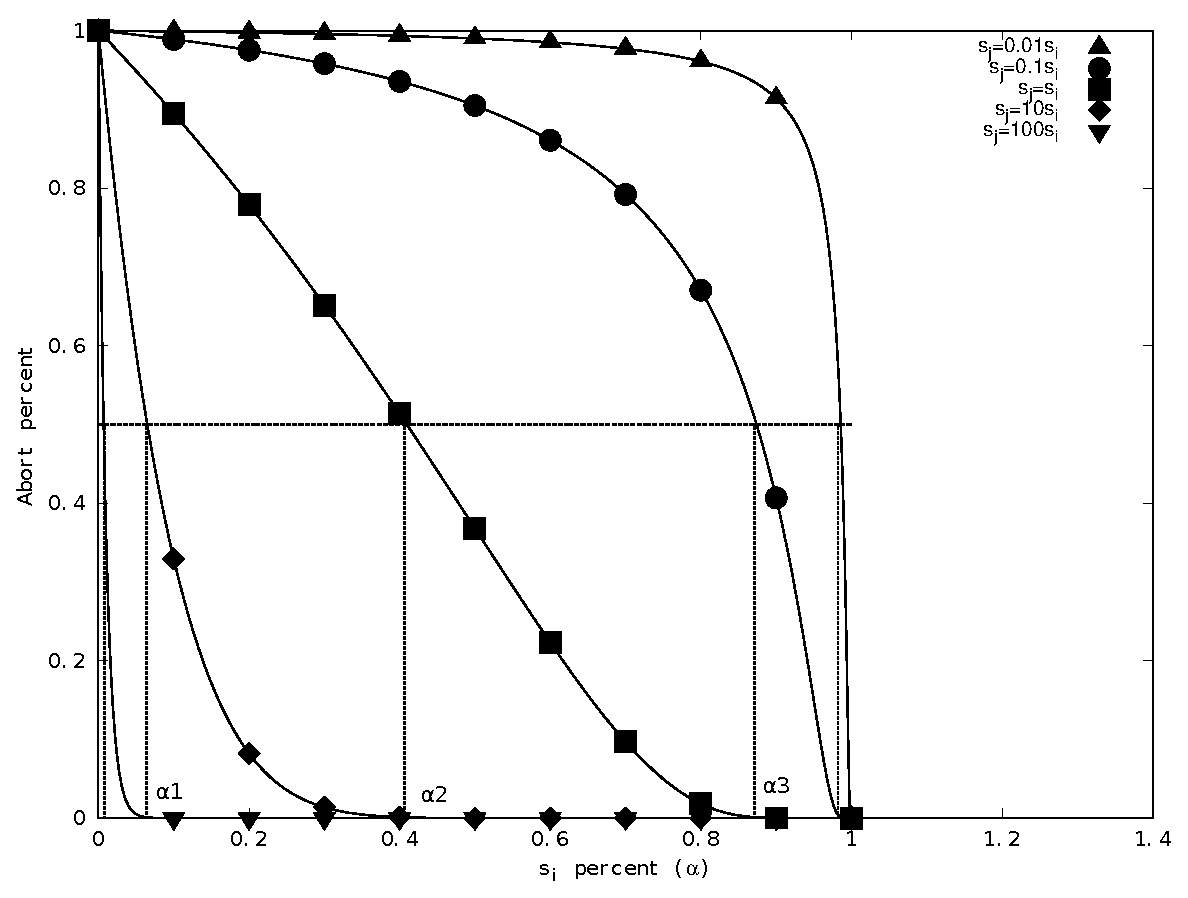
\includegraphics[scale=0.6]{figures/figure16}
\par\end{centering}

\caption{\label{fig16}Interference of $s_{i}^{k}(\theta)$ by various length
$s_{j}^{l}(\theta)$}
\end{figure}


Figure \ref{fig16} represents five different lengths of $s_{j}^{l}(\theta)$
interfering with $s_{i}^{k}(\theta)$ at all points of $s_{i}^{k}(\theta)$.
For a specific curve (which means a specific length for $s_{j}^{l}(\theta)$),
$\psi$ value determines the percentage of $len(s_{i}^{k}(\theta))$
above which $s_{i}^{k}(\theta)$ will be aborted. For example, for
$len(s_{j}^{l}(\theta))=0.1\times len(s_{i}^{k}(\theta))$, $s_{i}^{k}(\theta)$
will be aborted by $s_{j}^{l}(\theta)$ if the latter interferes with
$s_{i}^{k}(\theta)$ no later than $s_{i}^{k}(\theta)$ reaches $\alpha3$
percentages of its length. After that, $s_{j}^{l}(\theta)$ will have
to retry. As $len(s_{j}^{k}(\theta))$ decreases, the opportunity
that it will abort $s_{i}^{k}(\theta)$ at a higher percentage $\alpha_{max}$
increases, as $\alpha3>\alpha2>\alpha1$. The chosen function to represent
different curves in Figure \ref{fig16} is 
\begin{equation}
f(c_{m},\alpha)=e^{\frac{-c_{m}\alpha}{1-\alpha}}\label{eq49}
\end{equation}
where $c_{m}$ is fixed for a specific curve, but $\alpha$ changes
along each curve. This function acheives the desired requirements
that the abortion opportunity is reduced as $s_{i}^{k}(\theta)$ gets
closer to its end of execution (as $\alpha\rightarrow1,\, f(c_{m},1)\rightarrow0$),
or as the length of the conflicting transaction is large (as $c_{m}\rightarrow\infty,\, f(\infty,\alpha)\rightarrow0$).
Meanwhile, this abort opportunity is increased as $s_{i}^{k}(\theta)$
is interfered closer to its release (as $\alpha\rightarrow0,\, f(c_{m},0)\rightarrow1$),
or as length of conlicting transaction decreases (as $c_{m}\rightarrow0,\, f(0,\alpha)\rightarrow1$).
It should be noted that all lengths of $s_{i}^{k}(\theta)$ are normalized
to the same unit length, this way different values of $s_{j}^{l}(\theta)$
intercept different lengths of $s_{i}^{k}(\theta)$ at the same percentage
$\alpha_{max}^{jl}$ (the $\alpha$ value the corresponds the threshold
value $\psi$), but the actual length of interception for different
lengths of $s_{i}^{k}(\theta)$ differ according to $len(s_{i}^{k}(\theta))$
(i.e., let $len(s_{i}^{k}(\theta))\ne len(s_{i}^{k+1}(\theta))$,
then for one $s_{j}^{l}(\theta)$, both $s_{i}^{k}(\theta)$ and $s_{i}^{k+1}(\theta)$
will be intercepted at the same value $\alpha_{max}^{jl}$, but $\alpha_{max}len(s_{i}^{k}(\theta))$
differs from $\alpha_{max}len(s_{i}^{k+1}(\theta))$). This normalization
of different lengths of $s_{i}^{k}(\theta)$ is done to simplify calculations.

$s_{j}^{l}(\theta)$ belongs to a higher priority task than $s_{i}^{k}(\theta)$.
If $s_{j}^{l}(\theta)$ starts before or at the same start time of
$s_{i}^{k}(\theta)$, then $s_{i}^{k}(\theta)$ will have to abort
and retry until $s_{j}^{l}(\theta)$ finishes execution. But if $s_{j}^{l}(\theta)$
starts after $s_{i}^{k}(\theta)$, then the comparison illustrated
in Section \ref{sec 9.1} will be applied.

Let $s_{j}^{l}(\theta)$ interferes with $s_{i}^{k}(\theta)$ at $\alpha_{max}^{jl}$
percentage to acheive the threashold value $\psi$, then the maximum
retrial cost of $s_{i}^{k}(\theta)$ due to $s_{j}^{l}(\theta)$ is
\begin{equation}
\alpha_{max}^{jl}len(s_{i}^{k}(\theta))+len(s_{j}^{l}(\theta))\label{eq47}
\end{equation}
because if $s_{j}^{l}(\theta)$ interferes with $s_{i}^{k}(\theta)$
at a $\Upsilon$ percentage, where $\Upsilon<\alpha_{max}^{jl}$,
then the maximum retrial cost of $s_{i}^{k}(\theta)$ will be $\Upsilon len(s_{i}^{k}(\theta))+len(s_{j}^{l}(\theta))$
which is lower than that calculated in equation (\ref{eq47}). And
if $s_{j}^{l}(\theta)$ interferes with $s_{i}^{k}(\theta)$ after
$\alpha_{max}^{jl}$ percentage, then $s_{i}^{k}(\theta)$ will not
abort.

It should be noted that a higher priority task, $T_{j}$, can be blocked
by a lower priority one, $T_{i}$, if $s_{j}^{l}(\theta)$ interferes
with $s_{i}^{k}(\theta)$ after the the $\alpha_{max}^{jl}$ percentage.
This blocking time of $T_{j}$, due to $s_{i}^{k}(\theta)$ and $s_{j}^{l}(\theta)$,
is upper bounded by 
\begin{equation}
(1-\alpha_{max}^{jl})len(s_{i}^{k}(\theta))\label{eq48}
\end{equation}


\pagebreak{}


\section*{This part comes from the DATE12 paper, so it has some different notations
that that mentioned here, but it contains important information}

\begin{comment}
\textbackslash{}begin\{clm\} \textbackslash{}label\{priority\_inversion\}
A higher priority job, \$\textbackslash{}tau\_i\textasciicircum{}z\$,
suffers from priority inversion for at most number of atomic sections
in \$\textbackslash{}tau\_i\textasciicircum{}z\$. \textbackslash{}end\{clm\}
\textbackslash{}begin\{proof\} Assuming three atomic sections, \$s\_i\textasciicircum{}k(\textbackslash{}theta)\$,
\$s\_j\textasciicircum{}l(\textbackslash{}theta)\$ and \$s\_a\textasciicircum{}b(\textbackslash{}theta)\$,
where \$p\_j > p\_i\$ and \$s\_j\textasciicircum{}l(\textbackslash{}theta)\$
interferes with \$s\_i\textasciicircum{}k(\textbackslash{}theta)\$
after \$\textbackslash{}alpha\_\{ij\}\textasciicircum{}\{kl\}\$. Then
\$s\_j\textasciicircum{}l(\textbackslash{}theta)\$ will have to abort
and retry. At this time, if \$s\_a\textasciicircum{}b(\textbackslash{}theta)\$
interferes with the other two atomic sections, and the LCM decides
which transaction to commit based on comparison between each two transactions.
So, we have the following cases:- \textbackslash{}begin\{itemize\}
\textbackslash{}item \$p\_a < p\_i < p\_j\$, then \$s\_a\textasciicircum{}b(\textbackslash{}theta)\$
will not abort any one because it is still in its beginning and it
is of the lowest priority. So. \$\textbackslash{}tau\_j\$ is not indirectly
blocked by \$\textbackslash{}tau\_a\$. \textbackslash{}item \$p\_i<p\_a<p\_j\$
and even if \$s\_a\textasciicircum{}b(\textbackslash{}theta)\$ interferes
with \$s\_i\textasciicircum{}k(\textbackslash{}theta)\$ before \$\textbackslash{}alpha\_\{ia\}\textasciicircum{}\{kb\}\$,
so, \$s\_a\textasciicircum{}b(\textbackslash{}theta)\$ is allowed
abort \$s\_i\textasciicircum{}k(\textbackslash{}theta)\$. Comparison
between \$s\_j\textasciicircum{}l(\textbackslash{}theta)\$ and \$s\_a\textasciicircum{}b(\textbackslash{}theta)\$
will result in LCM choosing \$s\_j\textasciicircum{}l(\textbackslash{}theta)\$
to commit and abort \$s\_a\textasciicircum{}b(\textbackslash{}theta)\$
because the latter is still beginning, and \$\textbackslash{}tau\_j\$
is of higher priority. If \$s\_a\textasciicircum{}b(\textbackslash{}theta)\$
is not allowed to abort \$s\_i\textasciicircum{}k(\textbackslash{}theta)\$,
the situation is still the same, because \$s\_j\textasciicircum{}l(\textbackslash{}theta)\$
was already retrying until \$s\_i\textasciicircum{}k(\textbackslash{}theta)\$
finishes. \textbackslash{}item \$p\_a>p\_j>p\_i\$, then if \$s\_a\textasciicircum{}b(\textbackslash{}theta)\$
is chosen to commit, this is not priority inversion for \$\textbackslash{}tau\_j\$
because \$\textbackslash{}tau\_a\$ is of higher priority. \textbackslash{}item
if \$\textbackslash{}tau\_a\$ preempts \$\textbackslash{}tau\_i\$,
then LCM will compare only between \$s\_j\textasciicircum{}l(\textbackslash{}theta)\$
and \$s\_a\textasciicircum{}b(\textbackslash{}theta)\$. If \$p\_a<p\_j\$,
then \$s\_j\textasciicircum{}l(\textbackslash{}theta)\$ will commit
because of its task's higher priority and \$s\_a\textasciicircum{}b(\textbackslash{}theta)\$
is still at its beginning, otherwise, \$s\_j\textasciicircum{}l(\textbackslash{}theta)\$
will retry, but this will not be priority inversion because \$\textbackslash{}tau\_a\$
is already of higher priority than \$\textbackslash{}tau\_j\$. If
\$\textbackslash{}tau\_a\$ does not access any object but it preempts
\$\textbackslash{}tau\_i\$, then CM will choose \$s\_j\textasciicircum{}l(\textbackslash{}theta)\$
to commit as only already running transactions are competing together.
\textbackslash{}end\{itemize\} So, by generalizing these cases to
any number of conflicting jobs, it is seen that when an atomic section,
\$s\_j\textasciicircum{}l(\textbackslash{}theta)\$, of a higher priority
job is in conflict with a number of atomic sections belonging to lower
priority jobs, \$s\_j\textasciicircum{}l(\textbackslash{}theta)\$
can suffer from priority inversion by only one of them. So, each higher
priority job can suffer priority inversion at most its number of atomic
section. Claim follows. \textbackslash{}end\{proof\} 
\end{comment}


\pagebreak{}


\subsubsection{Response time of G-EDF/LCM}

By applying the same analogy used to derive equation (\ref{eq3}),
we find that $RC(T_{i})$ can be upper bounded by assuming each conflicting
atomic section, $s_{j}^{l}(\theta)$, causing a retry to the maximum
length atomic section that accesses object $\theta$, and this retry
will be $len(s_{j}^{l}(\theta))+\alpha_{max}^{jl}len(s_{max}(\theta))$,
where $\alpha_{max}^{jl}$ is the maximum percentage of $len(s_{max}(\theta))$
at which $s_{j}^{l}(\theta)$ forces $s_{max}(\theta)$ to retry.
But the subtracted $s_{max}(\theta)$ in equation (\ref{eq50}) will
be replaced by $\alpha_{max}^{*}s_{max}(\theta)$ where $\alpha_{max}^{*}=min_{\forall j,\forall l}\{\alpha_{max}^{jl}\}$,
because we are calculating the worst case retry cost, so the minimum
percentage of $len(s_{max}(\theta))$ should be the one to subtract.
Also, $s_{i_{max}}(\theta)$ is replaced by $\hat{\alpha}_{max}s_{i_{max}}(\theta)$
where $\hat{\alpha}_{max}$ is the maximum percentage of $len(s_{i_{max}}(\theta))$
at which any of the conflicting atomic sections will enforce $s_{i_{max}}(\theta)$
to retry. So, equation (\ref{eq50}) will be 

\begin{eqnarray}
RC(t(T_{i})) & \le & \sum_{\theta\in\theta_{i}}((\sum_{T_{j}\in\gamma(\theta)}(\lceil\frac{t(T_{i})}{t(T_{j})}\rceil\sum_{\forall s_{j}^{l}(\theta)}len(s_{j}^{l}(\theta))+\alpha_{max}^{jl}len(s_{max}(\theta))))\nonumber \\
 &  & -\alpha_{max}^{*}len(s_{max}(\theta))+\hat{\alpha}_{max}len(s_{i_{max}}(\theta)))\label{eq50}
\end{eqnarray}


The same way, equation (\ref{eq4}) will be 
\begin{eqnarray}
RC(t(T_{i})) & \le & \sum_{\theta\in\theta_{i}}((\sum_{T_{j}\in\gamma(\theta)}(\lceil\frac{t(T_{i})}{t(T_{j})}\rceil\sum_{\forall s_{j}^{l}(\theta)}len(s_{j}^{l}(\theta))+\alpha_{max}^{jl}len(s_{max}^{*}(\theta))))\nonumber \\
 &  & -\alpha_{max}^{*}len(\bar{s}_{max}(\theta))+\hat{\alpha}_{max}len(s_{i_{max}}(\theta)))\label{eq51}
\end{eqnarray}
and $RC(T_{i})$ will be calculated as in equation (\ref{eq5}) but
with using equations (\ref{eq50},\ref{eq51}) for each object $\theta$
instead of equations (\ref{eq3},\ref{eq4}) to get equation (\ref{eq53}).

\begin{equation}
RC(t(T_{i}))\le\sum_{\theta\in\theta_{i}}min\begin{cases}
\begin{cases}
((\sum_{T_{j}\in\gamma(\theta)}(\lceil\frac{t(T_{i})}{t(T_{j})}\rceil\sum_{\forall s_{j}^{l}(\theta)\in s_{j}(\theta)}len(s_{j}^{l}(\theta))+\alpha_{max}^{jl}len(s_{max}(\theta))))\\
\alpha_{max}^{*}len(s_{max}(\theta))+\hat{\alpha}_{max}len(s_{i_{max}}(\theta)))
\end{cases}\\
\\
\begin{cases}
((\sum_{T_{j}\in\gamma(\theta)}(\lceil\frac{t(T_{i})}{t(T_{j})}\rceil\sum_{\forall s_{j}^{l}(\theta)\in s_{j}(\theta)}len(s_{j}^{l}(\theta))+\alpha_{max}^{jl}len(s_{max}^{*}(\theta))))\\
-\alpha_{max}^{*}len(\bar{s}_{max}(\theta))+\hat{\alpha}_{max}len(s_{i_{max}}(\theta)))
\end{cases}\\
\\
\end{cases}\label{eq53}
\end{equation}


To get a tighter retry cost, the same rationale of equation (\ref{eq15})
can be used to get equation (\ref{eq52})

\begin{equation}
RC(t(T_{i}))\le\sum_{\theta\in\theta_{i}}min\begin{cases}
\begin{cases}
((\sum_{T_{j}\in\gamma(\theta)}(\sum_{\forall s_{j}^{l^{*}}(\theta)}len(s_{j}^{l^{*}}(\theta))+\alpha_{max}^{jl}len(s_{max}(\theta)))+\\
(\lfloor\frac{t(T_{i})}{t(T_{j})}\rfloor\sum_{\forall s_{j}^{l}(\theta)}len(s_{j}^{l}(\theta))+\alpha_{max}^{jl}len(s_{max}(\theta))))-\alpha_{max}^{*}len(s_{max}(\theta))+\hat{\alpha}_{max}len(s_{i_{max}}(\theta)))
\end{cases}\\
\\
\begin{cases}
((\sum_{T_{j}\in\gamma(\theta)}(\sum_{\forall s_{j}^{l^{*}}(\theta)}len(s_{j}^{l^{*}}(\theta))+\alpha_{max}^{jl}len(s_{max}^{*}(\theta)))+\\
(\lceil\frac{t(T_{i})}{t(T_{j})}\rceil\sum_{\forall s_{j}^{l}(\theta)}len(s_{j}^{l}(\theta))+\alpha_{max}^{jl}len(s_{max}^{*}(\theta))))-\alpha_{max}^{*}len(\bar{s}_{max}(\theta))+\hat{\alpha}_{max}len(s_{i_{max}}(\theta)))
\end{cases}\\
\\
\end{cases}\label{eq52}
\end{equation}


As was said in Section \ref{sec 9.1}, $T_{i}$ can be blocked by
a lower priority task $T_{h}$, if an atomic section of $T_{i}$,
$s_{i}^{k}(\theta)$ interferes with one of the atomic sections in
$T_{h}$,$s_{h}^{z}(\theta)$, after the maximum allowed percentage
of $len(s_{h}^{z}(\theta))$, then, $s_{i}^{k}(\theta)$ will abort
and retry until $s_{h}^{z}(\theta)$ finishes.

Let $T_{i}^{x}$ be the studied instance of $T_{i}$. For the case
of G-EDF, there can be at most only one instance of $T_{h}$, $T_{h}^{v}$,
during $t(T_{i})$, that can have a lower priority (larger absolute
deadline) than $T_{i}^{x}$. As it was shown that the worst interference
pattern of $T_{h}$ to $T_{i}$ occurs when the absolute deadline
of one instance of $T_{h}$, $T_{h}^{p}$, coincides with the absolute
deadline of $T_{i}^{x}$. This means that the $T_{h}^{p+1}$ will
be the first instance of $T_{h}$ with lower priority than $T_{i}^{x}$,
but $T_{h}^{p+1}$ will be released after $d(T_{i}^{x})$, so it will
not block $T_{i}^{x}$. So, to get the instance of $T_{h}$ that can
block $T_{i}^{x}$, the worst interference pattern is shifted a little
to the right, as shown in Figure \ref{fig17-b}, so that $T_{h}^{p}$
will be a carried-out job that can block $T_{i}^{x}$.

\begin{figure}
\subfloat[\label{fig17-a}No blocking to $T_{i}$]{\begin{centering}
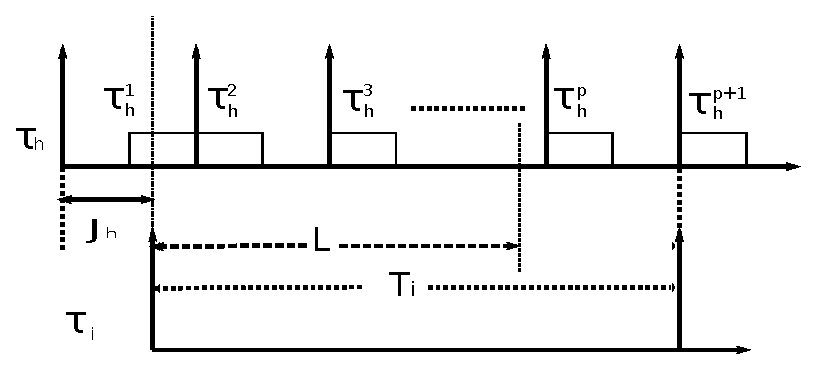
\includegraphics[scale=0.5]{figures/figure17-a}
\par\end{centering}

}

\subfloat[\label{fig17-b}Blocking to $T_{i}$ by $T_{h}^{p}$]{\begin{centering}
\includegraphics[scale=0.5]{figures/figure17-b}
\par\end{centering}

}

\caption{\label{fig17}Interference to $T_{i}$ by higher and lower priority
tasks}
\end{figure}
So, we have two cases for $T_{i}$. The first one shown in Figure
\ref{fig17-a} which represents the worst case interference pattern
of $T_{h}$ to $T_{i}$. $T_{i}$ does not suffer blocking because
$T_{h}^{p+1}$ is released after the absolute deadline of $T_{i}^{x}$,
but $T_{i}^{x}$ sufferes only from retry cots due to instances $T_{h}^{1}$
to $T_{h}^{p}$, and the retry cost is given in equation (\ref{eq57})
and its tighter form (\ref{eq52}). The other case is shown in Figure
\ref{fig17-b}, where the interference pattern in Figure \ref{fig17-a}
is shifted to the right, so priority of $T_{h}^{p}$ is lower than
that of $T_{i}^{x}$. So, $T_{i}^{x}$ suffers retry cost due to instances
$T_{h}^{1}$ to $T_{h}^{p-1}$, and suffers blocking (as in equation
(\ref{eq48})) due to instance $T_{h}^{p}$. Any further instance
than $T_{h}^{p}$ cannot block $T_{i}^{x}$ because they all start
after $d(T_{i}^{x})$. The retry and blocking costs of $T_{i}$ can
be obtained by modifying equation (\ref{eq57}) to include only instances
$T_{h}^{1}$ to $T_{h}^{p-1}$ in the retry cost, and $T_{h}^{p}$
in the blocking cost. But as priority of $T_{i}^{x}$ is higher than
that of $T_{h}^{p}$, then any atomic section $s_{i}^{y}(\theta)$
in $T_{i}^{x}$ can be blocked by only one conflicting atomic section,
$s_{h}^{z}(\theta)$, of $T_{h}^{p}$. This is because after $s_{h}^{z}(\theta)$,
$s_{i}^{y}(\theta)$ will at most start at the same time as any further
conflicting atomic section in $T_{h}^{z}$, and as $s_{i}^{y}(\theta)$
belongs to a higher priority task, then the LCM -P will allow it to
commit first. On the other hand, one atomic section in $T_{h}$, $s_{h}^{z}(\theta)$,
can block multiple atomic sections in $T_{i}$ because any atomic
section with a suitable length in any other task can enforce $s_{h}^{z}(\theta)$
to retry multiple times, causing multiple atomic sections in $T_{i}$
to interfer with $s_{h}^{z}(\theta)$. So, the worst case for blocking
of $T_{i}^{x}$ by $T_{h}^{p}$ occurs if all atomic sections in $T_{i}^{x}$
that access a specific object $\theta$ are blocked by the maximum-length
atomic section in $T_{h}^{p}$ as shown in equation (\ref{eq55}).
\begin{equation}
B_{ih}\le\sum_{\forall s_{i}^{y}(\theta)}(1-\alpha_{max}^{iy})len(s_{h_{max}}(\theta))\label{eq55}
\end{equation}
where $\alpha_{max}^{iy}$ is the maximum percentage of $len(s_{h_{max}}(\theta))$
after which $s_{i}^{y}(\theta)$ will be enforced to abort and retry.

Thus, equation (\ref{eq53}) and its tighter form (\ref{eq52}) can
be modified to equation (\ref{eq57}) that includes the effect of
blocking. But as equation (\ref{eq57}) includes both retry and blocking
cost, it will be called $BR(T_{i})$.

\begin{equation}
BR(t(T_{i}))\le\sum_{\theta\in\theta_{i}}min\begin{cases}
\begin{cases}
((\sum_{T_{h}\in\gamma_{(\theta)}}(B_{ih}+\lfloor(\frac{t(T_{i})}{t(T_{h})}\rfloor\sum_{\forall s_{h}^{z}(\theta)}len(s_{h}^{z}(\theta))+\alpha_{max}^{hz}len(s_{max}(\theta))))\\
-\alpha_{max}^{*}len(s_{max}(\theta))+\hat{\alpha}_{max}len(s_{i_{max}}(\theta)))
\end{cases}\\
\\
\begin{cases}
((\sum_{T_{h}\in\gamma_{(\theta)}}(B_{ih}+\lfloor\frac{t(T_{i})}{t(T_{h})}\rfloor\sum_{\forall s_{h}^{z}(\theta)}len(s_{h}^{z}(\theta))+\alpha_{max}^{hz}len(s_{max}^{*}(\theta))))\\
-\alpha_{max}^{*}len(\bar{s}_{max}(\theta))+\hat{\alpha}_{max}len(s_{i_{max}}(\theta)))
\end{cases}\\
\\
\end{cases}\label{eq54}
\end{equation}
To get the total effect of $T_{h}$ on $T_{i}$, we take the maximum
cost between retry without blocking and retry with blocking that each
$T_{h}^{p}$ imposes on $T_{i}^{x}$. But as equation (\ref{eq54})
calculates costs depending on each object $\theta$, then a task $T_{h}$
may produce a maximum effect on $T_{i}$ for a specific object $\theta_{1}$
if it induces no blocking, but for another object $\theta_{2}$, it
induces blocing on $T_{i}$ to get the maximum cost, but $T_{h}$
cannot be in the two positions for the same $T_{i}$. This why equation
(\ref{eq54}) should be calculated based on each task $T_{h}$, not
on each object $\theta\in\theta_{i}$. This modification also applies
to equations (\ref{eq53},\ref{eq52}). Thus, the final cost imposed
by all $T_{h}$ on $T_{i}$ (this cost will be called $CO(t(T_{i}))$)
will be calculated by equation (\ref{eq56}) depending on equations
(\ref{eq53},\ref{eq54}), or by equation (\ref{eq57}) depending
on equation (\ref{eq52}) (the tighter form of equation (\ref{eq53}))
and equation (\ref{eq54}).

\begin{equation}
CO(t(T_{i}))\le\sum_{T_{h}\in\gamma_{i}}max\begin{cases}
min\begin{cases}
\begin{cases}
((\sum_{\theta\in\theta_{i}\wedge\theta_{h}}(\lceil\frac{t(T_{i})}{t(T_{h})}\rceil\sum_{\forall s_{h}^{z}(\theta)}len(s_{h}^{z}(\theta))+\alpha_{max}^{hz}len(s_{max}(\theta))))\\
-\alpha_{max}^{*}len(s_{max}(\theta))+\hat{\alpha}_{max}len(s_{i_{max}}(\theta)))
\end{cases}\\
\begin{cases}
((\sum_{\theta\in\theta_{i}\wedge\theta_{h}}(\lceil\frac{t(T_{i})}{t(T_{h})}\rceil\sum_{\forall s_{h}^{z}(\theta)}len(s_{h}^{z}(\theta))+\alpha_{max}^{hz}len(s_{max}^{*}(\theta))))\\
-\alpha_{max}^{*}len(\bar{s}_{max}(\theta))+\hat{\alpha}_{max}len(s_{i_{max}}(\theta)))
\end{cases}
\end{cases}\\
min\begin{cases}
\begin{cases}
((\sum_{\theta\in\theta_{i}\wedge\theta_{h}}(B_{ih}+\lfloor(\frac{t(T_{i})}{t(T_{h})}\rfloor\sum_{\forall s_{h}^{z}(\theta)}len(s_{h}^{z}(\theta))+\alpha_{max}^{hz}len(s_{max}(\theta))))\\
-\alpha_{max}^{*}len(s_{max}(\theta))+\hat{\alpha}_{max}len(s_{i_{max}}(\theta)))
\end{cases}\\
\begin{cases}
((\sum_{\theta\in\theta_{i}\wedge\theta_{h}}(B_{ih}+\lfloor\frac{t(T_{i})}{t(T_{h})}\rfloor\sum_{\forall s_{h}^{z}(\theta)}len(s_{h}^{z}(\theta))+\alpha_{max}^{hz}len(s_{max}^{*}(\theta))))\\
-\alpha_{max}^{*}len(\bar{s}_{max}(\theta))+\hat{\alpha}_{max}len(s_{i_{max}}(\theta)))
\end{cases}
\end{cases}
\end{cases}\label{eq56}
\end{equation}


\begin{equation}
CO(t(T_{i}))\le\sum_{T_{h}\in\gamma_{i}}max\begin{cases}
min\begin{cases}
\begin{cases}
((\sum_{\theta\in\theta_{i}\wedge\theta_{h}}(\sum_{\forall s_{h}^{z^{*}}(\theta)}len(s_{h}^{z^{*}}(\theta))+\alpha_{max}^{hz}len(s_{max}(\theta)))+\\
(\lfloor\frac{t(T_{i})}{t(T_{h})}\rfloor\sum_{\forall s_{h}^{z}(\theta)}len(s_{h}^{z}(\theta))+\alpha_{max}^{hz}len(s_{max}(\theta))))-\alpha_{max}^{*}len(s_{max}(\theta))+\hat{\alpha}_{max}len(s_{i_{max}}(\theta)))
\end{cases}\\
\begin{cases}
((\sum_{\theta\in\theta_{i}\wedge\theta_{h}}(\sum_{\forall s_{h}^{z^{*}}(\theta)}len(s_{h}^{z^{*}}(\theta))+\alpha_{max}^{hz}len(s_{max}^{*}(\theta)))+\\
(\lceil\frac{t(T_{i})}{t(T_{h})}\rceil\sum_{\forall s_{h}^{z}(\theta)}len(s_{h}^{z}(\theta))+\alpha_{max}^{hz}len(s_{max}^{*}(\theta))))-\alpha_{max}^{*}len(\bar{s}_{max}(\theta))+\hat{\alpha}_{max}len(s_{i_{max}}(\theta)))
\end{cases}
\end{cases}\\
min\begin{cases}
\begin{cases}
((\sum_{\theta\in\theta_{i}\wedge\theta_{h}}(B_{ih}+\lfloor(\frac{t(T_{i})}{t(T_{h})}\rfloor\sum_{\forall s_{h}^{z}(\theta)}len(s_{h}^{z}(\theta))+\alpha_{max}^{hz}len(s_{max}(\theta))))\\
-\alpha_{max}^{*}len(s_{max}(\theta))+\hat{\alpha}_{max}len(s_{i_{max}}(\theta)))
\end{cases}\\
\begin{cases}
((\sum_{\theta\in\theta_{i}\wedge\theta_{h}}(B_{ih}+\lfloor\frac{t(T_{i})}{t(T_{h})}\rfloor\sum_{\forall s_{h}^{z}(\theta)}len(s_{h}^{z}(\theta))+\alpha_{max}^{hz}len(s_{max}^{*}(\theta))))\\
-\alpha_{max}^{*}len(\bar{s}_{max}(\theta))+\hat{\alpha}_{max}len(s_{i_{max}}(\theta)))
\end{cases}
\end{cases}
\end{cases}\label{eq57}
\end{equation}


Costs of $T_{i}$ can be calculated over an interval $L(T_{i})\le\lfloor\frac{t(T_{i})-c_{h}}{t(T_{h})}\rfloor t(T_{h})+c_{h}$
(which can be deduced from Figure \ref{fig17-b}) to get a tighter
upper bound on response time. But during this $L(T_{i})$ duration,
$T_{i}$ will not be blocked by any instance of $T_{h}$ because of
higher priority of all $T_{h}^{p}$ during $L(T_{i})$ than $T_{i}^{x}$.
If $L(T_{i})$ is increased over its specified limit, then costs of
$T_{i}$ can be calculated by equation (\ref{eq54}) where the last
instance of $T_{h}$ blocks $T_{i}^{x}$, but equation (\ref{eq54})
is already included in $CO(T_{i})$, so there is no need to increase
$L(T_{i})$ over its pecified limit. So, the costs of $T_{i}$ over
$L(T_{i})$ can be obtained from equation (\ref{eq16}), with some
modifications to account for LCM -P, and this will result in equation
(\ref{eq58})
\begin{equation}
RC(L(T_{i}))=\sum_{\theta\in\theta_{i}}min\begin{cases}
\begin{cases}
((\sum_{T_{h}\in\gamma(\theta)}((\lceil\frac{L-c_{h}}{t(T_{h})}\rceil+1)\sum_{\forall s_{h}^{z}(\theta)}len(s_{h}^{z}(\theta))\\
+\alpha_{max}^{hz}len(s_{max}(\theta))))-\alpha_{max}^{*}len(s_{max}(\theta))+\hat{\alpha}_{max}len(s_{i_{max}}(\theta)))
\end{cases}\\
\begin{cases}
((\sum_{T_{h}\in\gamma(\theta)}((\lceil\frac{L-c_{h}}{t(T_{h})}\rceil+1)\sum_{\forall s_{h}^{z}(\theta)}len(s_{h}^{z}(\theta))\\
+\alpha_{max}^{hz}len(s_{max}^{*}(\theta))))-\alpha_{max}^{*}len(\bar{s}_{max}(\theta))+\hat{\alpha}_{max}len(s_{i_{max}}(\theta)))
\end{cases}
\end{cases}\label{eq58}
\end{equation}
So, the final costs of $T_{i}$, $CO(T_{i})$, can be calculated by
equation (\ref{eq59}).
\begin{equation}
CO(T_{i})=\begin{cases}
RC(L(T_{i})) & if\, L(T_{i})\le\lfloor\frac{t(T_{i})-c_{h}}{t(T_{h})}\rfloor t(T_{h})+c_{h}\\
CO(t(T_{i})) & otherwise
\end{cases}\label{eq59}
\end{equation}
and response time of $T_{i}$ can be calculated by equation (\ref{eq10})
but $RC(T_{i})$ will be replaced with $CO(T_{i})$.


\subsubsection{\label{sub:Comparison-between-G-EDF/EDF}G-EDF/LCM versus ECM}

Execution time of each task $T_{i}$ , in G-EDF/LCM, is inflated by
addingt $CO(T_{i})$ to $c_{i}$, and in ECM, by adding $RC(T_{i})$
to $c_{i}$. Then, total utilization between ECM and G-EDF/LCM are
compared to know when G-EDF/LCM will be better as follows :-

\begin{eqnarray*}
\sum_{\forall T_{i}}\frac{c_{i}+CO(T_{i})}{t(T_{i})} & \le & \sum_{\forall T_{i}}\frac{c_{i}+RC(T_{i})}{t(T_{i})}\\
\sum_{\forall T_{i}}\frac{CO(T_{i})}{t(T_{i})} & \le & \sum_{\forall T_{i}}\frac{RC(T_{i})}{t(T_{i})}
\end{eqnarray*}


But the $RC(T_{i})$ is upper bounded by equation (\ref{eq30})
\begin{equation}
RC(T_{i})\le\sum_{T_{h}\in\gamma_{i}}(\sum_{\theta\in\theta_{i}\wedge\theta_{h}}(\lceil\frac{t(T_{i})}{t(T_{h})}\rceil\sum_{\forall s_{h}^{z}(\theta)}(2.s_{max})))\label{eq61}
\end{equation}
with the same assumptions that $s_{h}^{l}(\theta)$, $s_{max}(\theta)$,
$s_{i_{max}}(\theta)$, $s_{max}^{*}(\theta)$ and $\bar{s}_{max}(\theta)$
are replaced by $s_{max}$. With the same assumptions, $CO(T_{i})$
can also be upper bounded by 
\begin{equation}
CO(T_{i})\le\sum_{T_{h}\in\gamma_{i}}max\begin{cases}
(\sum_{\theta\in\theta_{i}\wedge\theta_{h}}(\lceil\frac{t(T_{i})}{t(T_{h})}\rceil\sum_{\forall s_{h}^{z}(\theta)}(1+\alpha_{max})s_{max}))\\
(\sum_{\theta\in\theta_{i}\wedge\theta_{h}}((\sum_{\forall s_{i}^{y}(\theta)}(1-\alpha_{min})s_{max})+\lfloor\frac{t(T_{i})}{t(T_{h})}\rfloor\sum_{\forall s_{h}^{z}(\theta)}(1+\alpha_{max})s_{max}))
\end{cases}\label{eq62}
\end{equation}
where all atomic sections are replaced by $s_{max}$, hence $\alpha$
will be the same for all atomic sections and will be called $\alpha_{max}$.
So, $s_{max}$ and $\alpha_{max}$ are both constants. If $\sum_{\theta\in\theta_{i}\wedge\theta_{h}}\sum_{\forall s_{h}^{z}(\theta)}$
and $\sum_{\theta\in\theta_{i}\wedge\theta_{h}}\sum_{\forall s_{i}^{y}(\theta)}$
are both lower than $\beta_{i,h}$, which is the maximum access number
of all shared objects by both $T_{i}$ and $T_{h}$. So, equation
(\ref{eq61}) will be
\begin{equation}
RC(T_{i})\le\sum_{T_{h}\in\gamma_{i}}2\lceil\frac{t(T_{i})}{t(T_{h})}\rceil\beta_{i,h}s_{max}\label{eq63}
\end{equation}
and equation (\ref{eq62}) will be 
\begin{equation}
CO(T_{i})\le\sum_{T_{h}\in\gamma_{i}}max\begin{cases}
\beta_{i,h}\lceil\frac{t(T_{i})}{t(T_{h})}\rceil(1+\alpha_{max})s_{max}\\
((1-\alpha_{min})+\lfloor\frac{t(T_{i})}{t(T_{h})}\rfloor(1+\alpha_{max}))\beta_{i,h}s_{max}
\end{cases}\label{eq64}
\end{equation}


\textbf{\textit{In case }}$t(T_{i})=a_{ih}t(T_{h})$, then $\lceil\frac{t(T_{i})}{t(T_{h})}\rceil=\lfloor\frac{t(T_{i})}{t(T_{h})}\rfloor=a_{ih}$,
and equation (\ref{eq64}) will be
\begin{eqnarray}
CO(T_{i}) & \le & \sum_{T_{h}\in\gamma_{i}}max\begin{cases}
\beta_{i,h}a_{ih}(1+\alpha_{max})s_{max}\\
((1-\alpha_{min})+a_{ih}(1+\alpha_{max}))\beta_{i,h}s_{max}
\end{cases}\nonumber \\
 & \le & \sum_{T_{h}\in\gamma_{i}}((1-\alpha_{min})+a_{ih}(1+\alpha_{max}))\beta_{i,h}s_{max}\label{eq65}
\end{eqnarray}
and equation (\ref{eq63}) will be 
\[
RC(T_{i})\le\sum_{T_{h}\in\gamma_{i}}2a_{ih}\beta_{i,h}s_{max}
\]
Then, G-EDF/LCM will give better performance if 
\[
\sum_{\forall T_{i}}\frac{\sum_{T_{h}\in\gamma_{i}}((1-\alpha_{min})+a_{ih}(1+\alpha_{max}))\beta_{i,h}s_{max}}{t(T_{i})}\le\sum_{\forall T_{i}}\frac{\sum_{T_{h}\in\gamma_{i}}2a_{ih}\beta_{i,h}s_{max}}{t(T_{i})}
\]
This inequality is ensured if for each $T_{i}$ and $T_{h}$ 
\begin{eqnarray}
(1-\alpha_{min})+a_{ih}(1+\alpha_{max}) & \le & 2a_{ih}\nonumber \\
1-\alpha_{min} & \le & (1-\alpha_{max})a_{ih}\label{eq104}
\end{eqnarray}
If equation (\ref{eq104}) applies, then schedulability of G-EDF/LCM
is equal to or better than ECM.

\textbf{\textit{In case }}$t(T_{i})=a_{ih}t(T_{h})+\delta$, then
$\lfloor\frac{t(T_{i})}{t(T_{h})}\rfloor=a_{ih}$ and $\lceil\frac{t(T_{i})}{t(T_{h})}\rceil=a_{ih}+1$,
and equation (\ref{eq64}) will be
\begin{eqnarray}
CO(T_{i}) & \le & \sum_{T_{h}\in\gamma_{i}}max\begin{cases}
\beta_{i,h}(a_{ih}+1)(1+\alpha_{max})s_{max}\\
((1-\alpha_{min})+a_{ih}(1+\alpha_{max}))\beta_{i,h}s_{max}
\end{cases}\nonumber \\
 & \le & \sum_{T_{h}\in\gamma_{i}}\beta_{i,h}(a_{ih}+1)(1+\alpha_{max})s_{max}\label{eq66}
\end{eqnarray}
and equation (\ref{eq63}) will be 
\[
RC(T_{i})\le\sum_{T_{h}\in\gamma_{i}}2(a_{ih}+1)\beta_{i,h}s_{max}
\]
For G-EDF/LCM to be better than ECM, then
\[
\sum_{\forall T_{i}}\frac{\sum_{T_{h}\in\gamma_{i}}\beta_{i,h}(a_{ih}+1)(1+\alpha_{max})s_{max}}{t(T_{i})}\le\sum_{\forall T_{i}}\frac{\sum_{T_{h}\in\gamma_{i}}2(a_{ih}+1)\beta_{i,h}s_{max}}{t(T_{i})}
\]
This inequality is assured when for each $T_{i}$ and $T_{h}$
\begin{eqnarray*}
(a_{ih}+1)(1+\alpha_{max}) & \le & 2(a_{ih}+1)\\
1+\alpha_{max} & \le & 2\\
\alpha_{max} & \le & 1
\end{eqnarray*}
Because $\alpha_{max}$ is always less than or equal to 1, then performance
of G-EDF/LCM is better or equal to that of ECM for $t(T_{i})=a_{ih}t(T_{h})+\delta$.
So, for all cases, G-EDF/LCM gives better or equal performance to
that of ECM.


\subsubsection{Comparison between G-EDF/LCM and retry-loop lock-free algorithm}

\textbf{\textit{In case}} $t(T_{i})=a_{ih}t(T_{h})$, then $CO(T_{i})$
is upper bounded by equation (\ref{eq65}), and retry loop cost is
upper bounded by equation (\ref{eq32}). Total utilization of G-EDF/LCM
is compared to that of retry-loop lock-free algorithm to determine
which is better as follows :- 
\begin{eqnarray*}
\sum_{\forall T_{i}}\frac{\sum_{\forall T_{h}\in\gamma_{i}}((1-\alpha_{min})+a_{ih}(1+\alpha_{max}))\beta_{i,h}s_{max}}{t(T_{i})} & \le & \sum_{\forall T_{i}}\frac{\sum_{\forall T_{h}\in\gamma_{i}}(a_{ih}+1)\beta_{i,h}r_{max}}{t(T_{i})}
\end{eqnarray*}
\begin{eqnarray*}
\frac{s_{max}}{r_{max}} & \le & \frac{\sum_{\forall T_{i}}\frac{\sum_{\forall T_{h}\in\gamma_{i}}(a_{ih}+1).\beta_{i,h}}{t(T_{i})}}{\sum_{\forall T_{i}}\frac{\sum_{\forall T_{h}\in\gamma_{i}}((1-\alpha_{min})+a_{ih}(1+\alpha_{max}))\beta_{i,h}}{t(T_{i})}}
\end{eqnarray*}


By choosing $1-\alpha_{min}=a_{ih}(1-\alpha_{max})-\Delta a_{ih}$
, where $\Delta>0$, then schedulability of G-EDF/LCM is better than
schedulability of ECM, as shown by equation (\ref{eq104}) ($a_{ih}$
is at least 1 as there must be at least one instance of $T_{h}$ interfering
or blocking $T_{i}$, so $\Delta a_{ih}>0$)

$\therefore$

\begin{eqnarray*}
\frac{s_{max}}{r_{max}} & \le & \frac{\sum_{\forall T_{i}}\frac{\sum_{\forall T_{h}\in\gamma_{i}}(a_{ih}+1).\beta_{i,h}}{t(T_{i})}}{\sum_{\forall T_{i}}\frac{\sum_{\forall T_{h}\in\gamma_{i}}2a_{ih}\beta_{i,h}-\Delta a_{ih}\beta_{i,h}}{t(T_{i})}}\\
 & = & \frac{\sum_{\forall T_{i}}\frac{\sum_{\forall T_{h}\in\gamma_{i}}a_{ih}\beta_{i,h}}{t(T_{i})}+\sum_{\forall T_{i}}\frac{\sum_{\forall T_{h}\in\gamma_{i}}\beta_{i,h}}{t(T_{i})}}{\sum_{\forall T_{i}}\frac{\sum_{\forall T_{h}\in\gamma_{i}}2a_{ih}\beta_{i,h}(1-\Delta)}{t(T_{i})}}\\
 & = & \frac{1}{2(1-\Delta)}+\frac{\sum_{\forall T_{i}}\frac{\sum_{\forall T_{h}\in\gamma_{i}}\beta_{i,h}}{t(T_{i})}}{\sum_{\forall T_{i}}\frac{\sum_{\forall T_{h}\in\gamma_{i}}2a_{ih}\beta_{i,h}(1-\Delta)}{t(T_{i})}}
\end{eqnarray*}


Since $a_{ih}\ge1,\,\therefore$if $a_{ih}\rightarrow1,\,\therefore\,\frac{s_{max}}{r_{max}}\rightarrow\frac{1}{1-\Delta}>1$,
and as $a_{ih}\rightarrow\infty,\,\frac{s_{max}}{r_{max}}\rightarrow\frac{1}{2(1-\Delta)}>\frac{1}{2}$,
which means- by proper choice of $\Delta$- better values for length
of $s_{max}$ against $r_{max}$ compared with what was provided in
ECM \cite{stmconcurrencycontrol:emsoft11}.

\textbf{\textit{In case }}$t(T_{i})=a_{ih}t(T_{h})+\delta$, then
$CO(T_{i})$ is upper bounded by equation (\ref{eq66}), and comparison
between total utilization of G-EDF/LCM and retry-loop lock-free is:-

\begin{eqnarray*}
\sum_{\forall T_{i}}\frac{\sum_{T_{h}\in\gamma_{i}}\beta_{i,h}(a_{ih}+1)(1+\alpha_{max})s_{max}}{t(T_{i})} & \le\\
\sum_{\forall T_{i}}\frac{\sum_{\forall T_{h}\in\gamma_{i}}(a_{ih}+2)\beta_{i,h}r_{max}}{t(T_{i})}
\end{eqnarray*}
\begin{eqnarray*}
\frac{s_{max}}{r_{max}} & \le & \frac{\sum_{\forall T_{i}}\frac{\sum_{\forall T_{h}\in\gamma_{i}}(a_{ih}+2).\beta_{i,h}}{t(T_{i})}}{\sum_{\forall T_{i}}\frac{\sum_{T_{h}\in\gamma_{i}}\beta_{i,h}(a_{ih}+1)(1+\alpha_{max})}{t(T_{i})}}\\
 & = & \frac{\sum_{\forall T_{i}}\frac{\sum_{\forall T_{h}\in\gamma_{i}}(a_{ih}+1).\beta_{i,h}}{t(T_{i})}}{\sum_{\forall T_{i}}\frac{\sum_{T_{h}\in\gamma_{i}}\beta_{i,h}(a_{ih}+1)(1+\alpha_{max})}{t(T_{i})}}\\
 & + & \frac{\sum_{\forall T_{i}}\frac{\sum_{\forall T_{h}\in\gamma_{i}}\beta_{i,h}}{t(T_{i})}}{\sum_{\forall T_{i}}\frac{\sum_{T_{h}\in\gamma_{i}}\beta_{i,h}(a_{ih}+1)(1+\alpha_{max})}{t(T_{i})}}\\
 & = & \frac{1}{1+\alpha_{max}}+\frac{\sum_{\forall T_{i}}\frac{\sum_{\forall T_{h}\in\gamma_{i}}\beta_{i,h}}{t(T_{i})}}{\sum_{\forall T_{i}}\frac{\sum_{T_{h}\in\gamma_{i}}\beta_{i,h}(a_{ih}+1)(1+\alpha_{max})}{t(T_{i})}}
\end{eqnarray*}


If $a_{ih}\rightarrow1,\,\therefore\frac{s_{max}}{r_{max}}\le\frac{3}{2(1+\alpha_{max})}$,
if $\alpha_{max}\rightarrow0,\,\therefore\,\frac{s_{max}}{r_{max}}\le\frac{3}{2}>1$,
and if $\alpha_{max}\rightarrow1,\,\therefore\,\frac{s_{max}}{r_{max}}\le\frac{3}{4}>\frac{1}{2}$.
This means, in case of low interference and by choosing $\alpha_{max}$
small enough, length of $s_{max}$can be at most 1.5 length of $r_{max}$,
but if $\alpha_{max}$ is chosen large, length of $s_{max}$ can still
be larger than that provided by ECM ($0.75r_{max}$ in G-EDF/LCM against
$0.5r_{max}$ in ECM \cite{stmconcurrencycontrol:emsoft11}) 

If $a_{ih}\rightarrow\infty,\,\therefore\frac{s_{max}}{r_{max}}\le\frac{1}{1+\alpha_{max}}$,
if $\alpha_{max}\rightarrow0,\,\therefore\,\frac{s_{max}}{r_{max}}\le1$,
and if $\alpha_{max}\rightarrow1,\,\therefore\,\frac{s_{max}}{r_{max}}\le\frac{1}{2}$.
This means, in case of high interference, length of $s_{max}$ can
be as that provided by ECM (from $0.5r_{max}$ to $r_{max}$ \cite{stmconcurrencycontrol:emsoft11})


\subsubsection{Comparison between G-EDF/LCM and locking protocols}

Total utilization of G-EDF/LCM is compared against total utilization
of FMLP and OMLP locking protocols. As explained in Section \ref{sub:Comparison-between-FMLP},
blocking time of $T_{i}$ under FMLP is upper bounde by 
\begin{eqnarray}
B(T_{i}) & \le & |s\_\theta|_{max}\sum_{T_{i}}(N_{i,s}(m-1)\nonumber \\
 & + & (1+N_{i,l})max_{k\ne i}(N_{k,s}.(m-1)+1)\nonumber \\
 & + & N_{i,l}.(n-1).c1)\label{eq67}
\end{eqnarray}
where $|s\_\theta|_{max}$ is the maximum length for short resource
by any $T_{i}$, $N_{i,s}$ is the number of requests to short resources
by $T_{i}$, $N_{i,l}$ is the number of requests to long resources
by $T_{i}$, and $c1$ is a constant where the maximum length request
to any long resource by any $T_{i}$ equals $c1\times|s\_\theta|_{max}$.
Thus, this blocking time is $O(n(n+m))$.

In case $t(T_{i})=a_{ih}t(T_{h})$, then $CO(T_{i})$ is upper bounded
by equation (\ref{eq65}). By assuming $a_{ih}\le Const1$, where
$Const1$ is the maximum number of instances of any task $T_{h}$
in the period of any other task $T_{i}$, then $CO(T_{i})=O(n^{2})$.
In case $t(T_{i})=a_{ih}t(T_{h})+\delta$, then $CO(T_{i})$ is upper
bounded by equation (\ref{eq66}) which is also $O(n^{2})$.

So, for schedulability of G-EDF/LCM to be better or equal to that
of FMLP, total utilization of G-EDF/LCM, whether $t(T_{i})$ is an
integer multiple of $t(T_{h})$ or not, is compared against total
utilization of FMLP to give that 
\begin{eqnarray*}
\frac{s_{max}}{|s\_\theta|_{max}} & = & \frac{O(n(n+m))}{O(n^{2})}\\
 & = & O(\frac{m}{n})
\end{eqnarray*}
As mentioned in Section \ref{sec:Comparison-of-OMLP}, the blocking
time for $T_{i}$ is upper bounded by $2.(m-1).L_{max}\sum_{k=1}^{q}N_{i,k}$
which is $O(m)$, and the total utilization of a task set under OMLP
is $O(nm)$, but the total utilization under G-EDF/LCM is $O(n^{2})$.
So, by comparing total utilization of G-EDF/LCM and total utilization
of OMLP, we get
\[
\frac{s_{max}}{L_{max}}=O(\frac{m}{n})
\]
So, it is clear that G-EDF/LCM gives the same asymptotic schedulability
performance of ECM compared with locking protocols, and this is natural
as the difference between G-EDF/LCM and ECM is only when an atomic
section, $s_{h}^{z}(\theta)$, of a higher priority task is allowed
to abort an atomic section, $s_{i}^{l}(\theta)$, of a lower priority
task, while this abortion can happen at any point in the life time
of $s_{i}^{l}(\theta)$ in ECM, it is restricted in G-EDF/LCM.


\subsubsection{Response time in G-RMA/LCM}

Because of the fixed priority of G-RMA, all instances of the higher
priority task, $T_{j}$, can interfere with the lower priority task,
$T_{i}$, during $t(T_{i})$. So, blocking is not considered with
higher priority tasks than $T_{i}$, but blocking is considered for
all instances, during $t(T_{i})$, of any task, $T_{h}$, with lower
priority than $T_{i}$. Besides, whether response time is calculated
over all $t(T_{i})$, or over an interval $L<t(T_{i})$, the same
equations for costs of $T_{i}$ and response time will be used because
of fixed priority as shown in equation (\ref{eq60}).
\begin{eqnarray}
CO(L(T_{i})) & = & \sum_{\forall T_{j}^{*}}((\sum_{\theta\in(\theta_{i}\wedge\theta_{j})}((\lceil\frac{L-c_{j}}{t(T_{j})}\rceil+1).\sum_{\forall s_{j}^{l}(\theta)}len(s_{j}^{l}(\theta))+\alpha_{max}^{jl}len(s_{max}^{j}(\theta))))\nonumber \\
 & + & \sum_{\forall\bar{T}_{h}}\sum_{\theta\in(\theta_{i}\wedge\theta_{h})}((\lceil\frac{L-c_{h}}{t(T_{h})}\rceil+1).\sum_{\forall s_{i}^{y}(\theta)}(1-\alpha_{max}^{iy})len(s_{h_{max}}(\theta)))\label{eq60}
\end{eqnarray}
where $L(T_{i})$ can extend to $t(T_{i})$, and $s_{max}^{j}(\theta)$
is the maximum length atomic section accessing object $\theta$ among
all tasks of higher priority than $T_{i}$ and $T_{i}$ itself, $T_{j}^{*}=\{T_{j}|(T_{j}\in\gamma_{i})\wedge(p(T_{j})>p(T_{i}))\}$,
and $\bar{T}_{h}=\{T_{h}|(T_{h}\in\gamma_{i})\wedge(p(T_{h})<p(T_{i}))\}$

Response time can be calculated by equation (\ref{eq22}) with replacing
$RC(T_{i})$ with $CO(L(T_{i}))$.


\subsubsection{Comparison between G-RMA/LCM and RCM}

By applying the same assumptions in Section \ref{sub:Comparison-between-G-EDF/EDF},
equation (\ref{eq60}) can be upper bounded by 
\begin{eqnarray}
CO(L(T_{i})) & \le & \sum_{\forall T_{j}^{*}}(\sum_{\theta\in(\theta_{i}\wedge\theta_{j})}((\lceil\frac{t(T_{i})}{t(T_{j})}\rceil+1).\sum_{\forall s_{j}^{l}(\theta)}(1+\alpha_{max})len(s_{max})))\nonumber \\
 & + & \sum_{\forall\bar{T}_{h}}(\sum_{\theta\in(\theta_{i}\wedge\theta_{h})}((\lceil\frac{t(T_{i})}{t(T_{h})}\rceil+1).\sum_{\forall s_{i}^{y}(\theta)}(1-\alpha_{min})len(s_{max})))\nonumber \\
 & = & \sum_{\forall T_{j}^{*}}((\lceil\frac{t(T_{i})}{t(T_{j})}\rceil+1)(1+\alpha_{max})len(s_{max})\beta_{ij})\nonumber \\
 & + & \sum_{\forall\bar{T}_{h}}((\lceil\frac{t(T_{i})}{t(T_{h})}\rceil+1)(1-\alpha_{min})len(s_{max})\beta_{ih})\label{eq68}
\end{eqnarray}


where $\beta_{ij}$ is the number of access times by $T_{j}$ to shared
resources with $T_{i}$, and $\beta_{ih}$ is the same but between
$T_{i}$ and $T_{h}$. For RCM, $RC(T_{i})$ is upper bounded by
\begin{equation}
RC(T_{i})\le\sum_{\forall T_{j}^{*}}(\lceil\frac{t(T_{i})}{t(T_{j})}\rceil+1)2\beta_{ij}s_{max}\label{eq69}
\end{equation}


So, by comparing total utilization of G-RMA/LCM with that of RCM,
we get 
\begin{eqnarray*}
\sum_{\forall T_{i}}\frac{\sum_{\forall T_{j}^{*}}((\lceil\frac{t(T_{i})}{t(T_{j})}\rceil+1)(1+\alpha_{max})len(s_{max})\beta_{ij})+\sum_{\forall\bar{T}_{h}}((\lceil\frac{t(T_{i})}{t(T_{h})}\rceil+1)(1-\alpha_{min})len(s_{max})\beta_{ih})}{t(T_{i})}
\end{eqnarray*}


\[
\le\sum_{\forall T_{i}}\frac{\sum_{\forall T_{j}^{*}}(\lceil\frac{t(T_{i})}{t(T_{j})}\rceil+1)2\beta_{ij}len(s_{max})}{t(T_{i})}
\]


\begin{eqnarray*}
\sum_{\forall T_{i}}\frac{\sum_{\forall\bar{T}_{h}}(\lceil\frac{t(T_{i})}{t(T_{h})}\rceil+1)(1-\alpha_{min})\beta_{ih}}{t(T_{i})} & \le & \sum_{\forall T_{i}}\frac{\sum_{\forall T_{j}^{*}}(\lceil\frac{t(T_{i})}{t(T_{j})}\rceil+1)(1-\alpha_{max})\beta_{ij}}{t(T_{i})}\\
\frac{1-\alpha_{min}}{1-\alpha_{max}} & \le & \frac{\sum_{\forall T_{i}}\frac{\sum_{\forall T_{j}^{*}}(\lceil\frac{t(T_{i})}{t(T_{j})}\rceil+1)\beta_{ij}}{t(T_{i})}}{\sum_{\forall T_{i}}\frac{\sum_{\forall\bar{T}_{h}}(\lceil\frac{t(T_{i})}{t(T_{h})}\rceil+1)\beta_{ih}}{t(T_{i})}}
\end{eqnarray*}


$\because$G-RMA scheduler is used and it is assumed that relative
deadline of each task equals its period, and $T_{h}$ is of lower
priority than $T_{i}$, $\therefore\, t(T_{i})\le t(T_{h})$, $\therefore\,\lceil\frac{t(T_{i})}{t(T_{h})}\rceil=1$
for any $T_{i}$ and $T_{h}$. $\therefore$

\begin{equation}
\frac{1-\alpha_{min}}{1-\alpha_{max}}\le\frac{\sum_{\forall T_{i}}\frac{\sum_{\forall T_{j}^{*}}(\lceil\frac{t(T_{i})}{t(T_{j})}\rceil+1)\beta_{ij}}{t(T_{i})}}{2\sum_{\forall T_{i}}\frac{\sum_{\forall\bar{T}_{h}}\beta_{ih}}{t(T_{i})}}\label{eq70}
\end{equation}


So, if blocking time for each task $T_{i}$ is reduced, then the right
hand side of equation (\ref{eq70}) is increased, giving a larger
upper bound for $\frac{1-\alpha_{min}}{1-\alpha_{max}}$, and giving
a wider range for $\alpha_{min}$ and $\alpha_{max}$ to choose from.
So, by proper choice of $\alpha_{max}$ and $\alpha_{min}$, equation
(\ref{eq70}) can be applied, and schedulability performance of G-RMA/LCM
is better or equal to that of RCM.


\subsubsection{Comparison between G-RMA/LCM and retry-loop lock free algorithm}

$CO(T_{i})$ for G-RMA/LCM is upper bounded by equation (\ref{eq68}),
and $RC(T_{i})$ for retry-loop lock-free algorithm is upper bounded
by equation (\ref{eq32}) which is re-written here as
\begin{equation}
RC(T_{i})=\sum_{T_{v}\in\gamma_{i}}(\lceil\frac{t(T_{i})}{t(T_{v})}\rceil+1)\beta_{iv}r_{max}\label{eq72}
\end{equation}
But set of tasks $T_{v}\in\gamma_{i}$ are composed of tasks of higher
priority than $T_{i}$, which are donated as $T_{j}$ in consistence
to the index notation of G-RMA/LCM, and tasks of lower priority than
$T_{i}$, which are donated as $T_{h}$. So, equation (\ref{eq72})
can be re-written as equation (\ref{eq73}).
\begin{equation}
RC(T_{i})=\sum_{\forall T_{j}^{*}}(\lceil\frac{t(T_{i})}{t(T_{j})}\rceil+1)\beta_{ij}r_{max}+\sum_{\forall\bar{T_{h}}}(\lceil\frac{t(T_{i})}{t(T_{h})}\rceil+1)\beta_{ih}r_{max}\label{eq73}
\end{equation}


Assuming $\lambda_{3}(i,j)=(\lceil\frac{t(T_{i})}{t(T_{j})}\rceil+1)\beta_{ij}$
and $\chi_{3}(i,h)=(\lceil\frac{t(T_{i})}{t(T_{h})}\rceil+1)\beta_{ih}$.
So, to determine when schedulability performance of G-RMA/LCM will
be better or equal to that of retry-loop lock-free, we compare total
utilization of both as follows:-
\[
len(s_{max})\sum_{\forall T_{i}}\frac{\sum_{\forall T_{j}^{*}}(\lambda_{3}(i,j)(1+\alpha_{max}))+\sum_{\forall\bar{T}_{h}}(\chi_{3}(i,h)(1-\alpha_{min}))}{t(T_{i})}
\]


\[
\le r_{max}\sum_{\forall T_{i}}\frac{\sum_{T_{j}^{*}}\lambda_{3}(i,j)+\sum_{\bar{T}_{h}}\chi_{3}(i,h)}{t(T_{i})}
\]


$\therefore$

\begin{eqnarray*}
\frac{s_{max}}{r_{max}} & \le & \frac{\sum_{\forall T_{i}}\frac{\sum_{T_{j}^{*}}\lambda_{3}(i,j)+\sum_{\bar{T}_{h}}\chi_{3}(i,h)}{t(T_{i})}}{\sum_{\forall T_{i}}\frac{\sum_{\forall T_{j}^{*}}(\lambda_{3}(i,j)(1+\alpha_{max}))+\sum_{\forall\bar{T}_{h}}(\chi_{3}(i,h)(1-\alpha_{min}))}{t(T_{i})}}
\end{eqnarray*}


$\because$G-RMA scheduler is used and it is assumed that relative
deadline of each task equals its period, and $T_{h}$ is of lower
priority than $T_{i}$, $\therefore\, t(T_{i})\le t(T_{h})$, $\therefore\,\lceil\frac{t(T_{i})}{t(T_{h})}\rceil=1$
for any $T_{i}$ and $T_{h}$, $\therefore$

\begin{equation}
\frac{s_{max}}{r_{max}}\le\frac{\sum_{\forall T_{i}}\frac{\sum_{\forall T_{j}^{*}}\lambda_{x}(i,j)+2\sum_{\forall\bar{T}_{h}}\beta_{ih}}{t(T_{i})}}{\sum_{\forall T_{i}}\frac{\sum_{\forall T_{j}^{*}}(\lambda_{3}(i,j)(1+\alpha_{max}))+2\sum_{\forall\bar{T}_{h}}((1-\alpha_{min})\beta_{ih})}{t(T_{i})}}\label{eq74}
\end{equation}


If $\frac{s_{max}}{r_{max}}$ is kept lower or equal to $\frac{\sum_{\forall T_{i}}\frac{\sum_{\forall T_{j}^{*}}\lambda_{x}(i,j)+2\sum_{\forall\bar{T}_{h}}\beta_{ih}}{t(T_{i})}}{\sum_{\forall T_{i}}\frac{\sum_{\forall T_{j}^{*}}(\lambda_{3}(i,j)(1+\alpha_{max}))+2\sum_{\forall\bar{T}_{h}}((1+\alpha_{max})\beta_{ih})}{t(T_{i})}}$,
where $1-\alpha_{min}$ in denominator of the right hand side of inequality
(\ref{eq74}) is replaced by $1+\alpha_{max}$, then inequality (\ref{eq74})
is ensured because $\frac{\sum_{\forall T_{i}}\frac{\sum_{\forall T_{j}^{*}}\lambda_{x}(i,j)+2\sum_{\forall\bar{T}_{h}}\beta_{ih}}{t(T_{i})}}{\sum_{\forall T_{i}}\frac{\sum_{\forall T_{j}^{*}}(\lambda_{3}(i,j)(1+\alpha_{max}))+2\sum_{\forall\bar{T}_{h}}((1+\alpha_{max})\beta_{ih})}{t(T_{i})}}\le\frac{\sum_{\forall T_{i}}\frac{\sum_{\forall T_{j}^{*}}\lambda_{x}(i,j)+2\sum_{\forall\bar{T}_{h}}\beta_{ih}}{t(T_{i})}}{\sum_{\forall T_{i}}\frac{\sum_{\forall T_{j}^{*}}(\lambda_{3}(i,j)(1+\alpha_{max}))+2\sum_{\forall\bar{T}_{h}}((1-\alpha_{max})\beta_{ih})}{t(T_{i})}}$.
Thus, 
\begin{eqnarray}
\frac{s_{max}}{r_{max}} & \le & \frac{\sum_{\forall T_{i}}\frac{\sum_{\forall T_{j}^{*}}\lambda_{x}(i,j)+2\sum_{\forall\bar{T}_{h}}\beta_{ih}}{t(T_{i})}}{(1+\alpha_{max})\sum_{\forall T_{i}}\frac{\sum_{\forall T_{j}^{*}}\lambda_{3}(i,j)+2\sum_{\forall\bar{T}_{h}}\beta_{ih}}{t(T_{i})}}\label{eq76}\\
\therefore\frac{s_{max}}{r_{max}} & \le & \frac{1}{1+\alpha_{max}}\label{eq75}
\end{eqnarray}
As $0\le\alpha_{max}\le1$ and by proper choice of $\alpha_{max}$,
then the minimum upper bound on $\frac{s_{max}}{r_{max}}$ is higher
than 0.5, so length of $s_{max}$ can be kept higher than half length
of $r_{max}$, which is higher than that acheived in the specific
cases of RCM mentioned in Section \ref{sub:G-RMA-scheduler-with}
(actually, $\frac{s_{max}}{r_{max}}$ is a higher than $\frac{1}{1+\alpha_{max}}$
because the right hand side of inequality (\ref{eq74}) is the actual
upper limit to $\frac{s_{max}}{r_{max}}$, not the right hand side
of inequality (\ref{eq76})). But inequaltiy (\ref{eq75}) makes the
higher upper limit on $\frac{s_{max}}{r_{max}}$ is 1, which means
that the maximum allowed length to $s_{max}$- for performance of
G-RMA/LCM to better or equal to that of RCM- is the length of $r_{max}$,
but considering the special cases in Section \ref{sub:G-RMA-scheduler-with},
this can be changed as follows:-

It appears from inequality (\textbf{\uline{\Large \ref{eq74}}})
that $\frac{s_{max}}{r_{max}}$ depend on $\beta_{ij}$, $\beta_{ih}$,
$\lceil\frac{t(T_{i})}{t(T_{j})}\rceil$ and $\alpha_{max}$. The
minimum value for $\beta_{ij}$ and $\beta_{ih}$ is 1 as there must
be at least one shared resource between $T_{i},T_{j}$ and $T_{i},T_{h}$,
but $\beta_{ij}\rightarrow0$ means value of $\beta_{ij}$ is very
small compared to that of $\beta_{ih}$, and $\beta_{ih}\rightarrow0$
means the value of $\beta_{ih}$ is very small compared to that of
$\beta_{ij}$. Also, if $\beta_{ij}\rightarrow\infty$($\beta_{ih}\rightarrow\infty$),
then value of $\beta_{ij}$ ($\beta_{ih}$) is very large compared
to that of $\beta_{ih}$($\beta_{ij}$). If $\beta_{ij}\rightarrow\infty$
or $\beta_{ih}\rightarrow0$ (which can happen if higher priority
tasks tend to access shared resources much more compared with lower
priority tasks), then inequality (\ref{eq74}) $\rightarrow$ $\frac{s_{max}}{r_{max}}\le\frac{1}{1+\alpha_{max}}$,
which is the same as the general boundary from inequality (\ref{eq75}).
But if $\beta_{ij}\rightarrow0$ or $\beta_{ih}\rightarrow\infty$,
which happens if higher priority tasks tend to access shared resources
rarely compared to lower priority tasks , then inequality (\ref{eq74})
$\rightarrow\frac{s_{max}}{r_{max}}\le\frac{1}{1-\alpha_{max}}$,
and if $\alpha_{max}\rightarrow0$ (which means that an atomic section
$s_{j}^{l}(\theta)$ is only allowed to interfere another one $s_{i}^{k}(\theta)$
when $s_{i}^{k}(\theta)$ is very close to its start of execution),
then length of $s_{max}$ can be at most as that of $r_{max}$; the
physical interpretation of these parameters (i.e., $\beta_{ij}\rightarrow0$
or $\beta_{ih}\rightarrow\infty$ and $\alpha_{max}\rightarrow0$)
is that the effect of blocking in G-RMA/LCM is very large compared
to that of interference, and it is even increased by making $\alpha_{max}\rightarrow0$
which means that an atomic section $s_{j}^{l}(\theta)$, belonging
to a higher priority task $T_{j}$, would suffere the maximum blocking
time of any atomic section $s_{i}^{k}(\theta)$, belonging to a lower
priority task $T_{i}$, because $s_{j}^{l}(\theta)$ will have to
wait for almost the whole length of $s_{i}^{k}(\theta)$ in the worst
case of blocking, but as retry-loop lock-free also sufferes from lower
priority task whose effect is approximately the same as lower priority
tasks in G-RMA/LCM (as $\alpha_{max}\rightarrow0$), this will render
the lengths of $s_{max}$ and $r_{max}$ to be approximately the same
in order to make schedulability performance of G-RMA/LCM better or
equal to that of retry-loop lock-free method. But if $\alpha_{max}\rightarrow1$,
then $\frac{s_{max}}{r_{max}}\le\infty$ which means that length of
$s_{max}$ can be much greater than that of $r_{max}$. The physical
interpretation for these parameters (i.e., $\beta_{ij}\rightarrow0$
or $\beta_{ih}\rightarrow\infty$ and $\alpha_{max}\rightarrow1$)
is that the effect of blocking in G-RMA/LCM is very large compared
to effect of interference, but as $\alpha_{max}\rightarrow1$, then
at atomic section $s_{j}^{l}(\theta)$ will be blocked by another
one $s_{i}^{k}(\theta)$ for a very short time length (almost 0),
and this will reduce the effect of lower priority tasks too much,
in contrast to retry-loop lock-free algorithm where lower priority
tasks still affect retry cost, thus length of $s_{max}$ will be allowed
to be much greater than that of $r_{max}$ for schedulability performance
of G-RMA/LCM to be better or equal to that of retry-loop lock-free
algorithm.

If $\lceil\frac{t(T_{i})}{t(T_{j})}\rceil\rightarrow1$, then inequality
(\ref{eq74})$\rightarrow\frac{s_{max}}{r_{max}}\le\frac{\sum_{\forall T_{i}}\frac{2\sum_{(T_{j}\in\gamma_{i})\wedge(p(T_{j})>p(T_{i}))}\beta_{ij}+2\sum_{(T_{h}\in\gamma_{i})\wedge(p(T_{h})<p(T_{i}))}\beta_{ih}}{t(T_{i})}}{\sum_{\forall T_{i}}\frac{2(1+\alpha_{max})\sum_{(T_{j}\in\gamma_{i})\wedge(p(T_{j})>p(T_{i}))}\beta_{ij}+2(1-\alpha_{max})\sum_{(T_{h}\in\gamma_{i})\wedge(p(T_{h})<p(T_{i}))}\beta_{ih}}{t(T_{i})}}$, 

\[
\frac{s_{max}}{r_{max}}\le\frac{\sum_{\forall T_{i}}\frac{\sum_{\forall T_{j}^{*}}\lambda_{x}(i,j)+2\sum_{\forall\bar{T}_{h}}\beta_{ih}}{t(T_{i})}}{\sum_{\forall T_{i}}\frac{\sum_{\forall T_{j}^{*}}(\lambda_{3}(i,j)(1+\alpha_{max}))+2\sum_{\forall\bar{T}_{h}}((1-\alpha_{min})\beta_{ih})}{t(T_{i})}}
\]


which leaves the system under control of $\beta_{ij}$, $\beta_{ih}$
and $\alpha_{max}$ as explained above. But if $a_{ij}\rightarrow\infty$,
then inequaltiy (\ref{eq74})$\rightarrow\frac{s_{max}}{r_{max}}\le\frac{1}{1+\alpha_{max}}$
which is the same as the general boundary derived in inequality (\ref{eq75}).

From the previous analysis, it can be seen that G-RMA/LCM can acheive
the same value for $\frac{s_{max}}{r_{max}}$ as RCM, besides, it
can increase the minimum upper bound on $\frac{s_{max}}{r_{max}}$
- by proper choice of $\alpha_{max}$- from 0.5 in RCM to $\frac{1}{1+\alpha_{max}}$
in G-RMA/LCM.


\subsubsection{G-RMA/LCM versus OMLP}

As blocking time of $T_{i}$ under OMLP is upper bounded by $2.(m-1).L_{max}\sum_{k=1}^{q}N_{i,k}$
which is $O(m)$, so the total utilization of a task set under OMLP
is $O(nm)$, and the total utilization of a task set under G-RMA/LCM
is $O(n^{2})$. To determine when schedulability of G-RMA/LCM is better
or equal to that of OMLP, total utilization of G-RMA/LCM is compared
against that of OMLP (FMLP is not considered as it uses G-EDF for
scheduling) to get:-
\[
\frac{s_{max}}{L_{max}}=O(\frac{m}{n})
\]
So, if the available number of processors in the system is much greater
than number of tasks, $s_{max}$ is allowed to be much greater than
that of $L_{max}$.


\section{Experimental evaluation}

I THINK IN THIS PART I SHOULD MENTION WHAT RESULTS COMING OUT OF THE
EXPERIEMNTS (IN OTHER WORDS, WHAT THE QUESTIONS ANSWERED BY EXPERIEMNTS
ARE).


\subsection{Experiments setup}


\subsubsection{TALK ABOUT CHRONOS AND MODIFICATIONS BY R-STM, AND THE MODIFICATIONS
TO R-STM ITSELF (UNTIL NOW ALL EXPERIEMNTS ARE WRITE OPERATIONS).}

We used ChronOS real-time operating system \cite{dellinger2011chronos}
and Rochester STM implementation \cite{marathe2006lowering}, known
as RSTM . We modified the RSTM to include the new contention managers
ECM, RCM, LCM-EDF and LCM-RMA. For retry-loop lock-free implementation,
we use a loop that reads the value of a varible, then tries to write
a specified value in that variable using a CAS API provided by Rochester
University; if the CAS does not succeed, task loops until it can modify
the variable. We refer to this retry-loop lock-free operation as CAS-loop
operation.


\subsubsection{DESCRIPTION OF USED SERVERS.}

We use 8 core, 2GHz AMD Opeteron processor server. The average time
taken by one {}``write'' operation by RSTM implementation on any
core is 0.0129653375 \textbf{$\mu s$}, and the average time taken
by one {}``CAS-loop'' operation on any core is 0.0292546250 $\mu s$.


\subsubsection{DESCRIPTION OF TASK SETS.}

Three periodic task sets are used with time properties shown in Table
\ref{tab:Task-set-1}. Each task runs in its own thread and is modified
to include a random number of atomic sections by specifying three
parameters:- the maximum and minimum lengths of any atomic section
within the task, and the total length of atomic sections within any
task. Each parameter of the previous three ones takes a value of 0.2,
0.5 and 0.8 of the total length of the task, but of course, the minimum
length cannot exceed the maximum length, and both of them cannot exceed
the total lenght of atomic sections per task. IN THE CURRENT SET OF
EXPERIEMNTS, ALL TASKS MUST HAVE ATOMIC SECTIONS, AND ALL ATOMIC SECTION
ACCESS THE SAME OBJECT. In the current set of experiments, all atomic
sections try to make {}``write'' operations, so contention is at
its highest level. To compare STM against retry-loop lock-free method,
the same length of each atomic section within any task is implemented
with the CAS-loop operation. Due to the longer time taken by one CAS-loop,
the number of CAS-loops within the same length of atomic sections
is smaller than the number of {}``STM write'' operations within
the same length of atomic section, but using the same length of each
atomic section in comparing STM against retry-loop lock-free allowes
us to compare the effect of contention resolution between both methods,
ignoring the overhead of their implementations.

\begin{table}
\caption{\label{tab:Task-set-1}Task sets (a) \label{tab:Task-sets-(a)}Task
set 1 \label{tab:Task-sets-(b)}(b) Task set 2 \label{tab:Task-sets-(c)}(c)Task
set 3}


\centering{}%
\begin{tabular}{|c|c|c|}
\multicolumn{3}{c}{(a)}\tabularnewline
\cline{2-3} 
\multicolumn{1}{c|}{} & $T_{i}(\mu s)$ & $c_{i}(\mu s)$\tabularnewline
\hline 
$\tau_{1}$ & 500000 & 150000\tabularnewline
\hline 
$\tau_{2}$ & 1000000 & 227000\tabularnewline
\hline 
$\tau_{3}$ & 1500000 & 410000\tabularnewline
\hline 
$\tau_{4}$ & 3000000 & 299000\tabularnewline
\hline 
$\tau_{5}$ & 5000000 & 500000\tabularnewline
\hline 
\end{tabular} %
\begin{tabular}{|c|c|c|}
\multicolumn{3}{c}{(b)}\tabularnewline
\cline{2-3} 
\multicolumn{1}{c|}{} & $T_{i}(\mu s)$ & $c_{i}(\mu s)$\tabularnewline
\hline 
$\tau_{1}$ & 400000 & 75241\tabularnewline
\hline 
$\tau_{2}$ & 750000 & 69762\tabularnewline
\hline 
$\tau_{3}$ & 1200000 & 267122\tabularnewline
\hline 
$\tau_{4}$ & 1500000 & 69863\tabularnewline
\hline 
$\tau_{5}$ & 2400000 & 152014\tabularnewline
\hline 
$\tau_{6}$ & 4000000 & 286301\tabularnewline
\hline 
$\tau_{7}$ & 7500000 & 493150\tabularnewline
\hline 
$\tau_{8}$ & 10000000 & 794520\tabularnewline
\hline 
$\tau_{9}$ & 15000000 & 1212328\tabularnewline
\hline 
$\tau_{10}$ & 20000000 & 1775342\tabularnewline
\hline 
\end{tabular} %
\begin{tabular}{|c|c|c|}
\multicolumn{3}{c}{(c)}\tabularnewline
\cline{2-3} 
\multicolumn{1}{c|}{} & $T_{i}(\mu s)$ & $c_{i}(\mu s)$\tabularnewline
\hline 
$\tau_{1}$ & 400000 & 58195\tabularnewline
\hline 
$\tau_{2}$ & 750000 & 53963\tabularnewline
\hline 
$\tau_{3}$ & 1000000 & 206330\tabularnewline
\hline 
$\tau_{4}$ & 1200000 & 53968\tabularnewline
\hline 
$\tau_{5}$ & 1500000 & 117449\tabularnewline
\hline 
$\tau_{6}$ & 2400000 & 221143\tabularnewline
\hline 
$\tau_{7}$ & 3000000 & 290428\tabularnewline
\hline 
$\tau_{8}$ & 4000000 & 83420\tabularnewline
\hline 
$\tau_{9}$ & 7500000 & 380917\tabularnewline
\hline 
$\tau_{10}$ & 10000000 & 613700\tabularnewline
\hline 
$\tau_{11}$ & 15000000 & 936422\tabularnewline
\hline 
$\tau_{12}$ & 20000000 & 1371302\tabularnewline
\hline 
\end{tabular}
\end{table}



\subsubsection{Results}

Figure \ref{fig:RC_results} represents retry cost (RC) for each task
in the three task sets given in Table \ref{tab:Task-set-1} where
each task has one atomic section of length equal to half of its corresponding
task length. It can be seen that LCM-EDF and LCM-RMA acheive better
or comparative retry cost to ECM and RCM. As all tasks are initially
released at the same time, and due to time propereties of tasks as
shown in Table \ref{tab:Task-set-1}, this makes tasks with lower
ID somehow have higher priority when using G-EDF scheduler, meanwhile,
these tasks with lower ID are definitly of higher priority when using
G-RMA scheduling as tasks are ordered in non-decreasing periods. Thus,
it is seen that LCM-EDF and LCM-RMA acheive comparative retry cost
to ECM and RCM for some tasks with lower ID, but as task ID increases,
LCM - for both schedulers- acheive much better results than ECM and
RCM. This is because higher priority tasks in LCM suffers blocking
by lower priority tasks, which is not the case for ECM and RCM, but
as task priority decreases, LCM, by definition, pervents higher priority
tasks from aborting lower priority ones if the higher priority task
interfers with a lower priority one after a specified threshold, but
for ECM and RCM, lower priority tasks must abort in favor of higher
priority ones. LCM-EDF and LCM-RMA also acheive comparative or better
results than retry-loop lock-free algorithm.

\begin{figure}
\subfloat[\label{fig-RC-set1}Task set 1]{\begin{centering}
\includegraphics[scale=0.5]{/e/lectures/real-time/PhD-work/stm/Practical/results_uno/figures/Abr_Dur/Abr_dur_5t_nl_g_30_0\lyxdot 5_0\lyxdot 5_0\lyxdot 5_1}
\par\end{centering}



}

\subfloat[\label{fig-RC-set2}Task set 2]{\begin{centering}
\includegraphics[scale=0.5]{/e/lectures/real-time/PhD-work/stm/Practical/results_uno/figures/Abr_Dur/Abr_dur_10t_nl_g_30_0\lyxdot 5_0\lyxdot 5_0\lyxdot 5_1}
\par\end{centering}

}

\subfloat[\label{fig-RC-set3}Task set 3 ]{\begin{centering}
\includegraphics[scale=0.5]{/e/lectures/real-time/PhD-work/stm/Practical/results_uno/figures/Abr_Dur/Abr_dur_12t_nl_g_30_0\lyxdot 5_0\lyxdot 5_0\lyxdot 5_1}
\par\end{centering}



}

\caption{\label{fig:RC_results}Retry Cost by nano\_sec for each task in a)Task
set 1 b)Task set 2 c)Task set 3}
\end{figure}


Figure \ref{fig:res_results-1} shows response time of each task in
the three task sets given in Table \ref{tab:Task-set-1} where each
task has one atomic section of length equals to half of its corresponding
task. It appears from Figure \ref{fig:res_results-1} that LCM-EDF
and LCM-RMA acheive better response time than retry-loop lock-free
algorithm, and comparative or better response time than ECM and RCM.

\begin{figure}
\subfloat[\label{fig-res-set1-1}Task set 1]{\begin{centering}
\includegraphics[scale=0.5]{/e/lectures/real-time/PhD-work/stm/Practical/results_uno/figures/Res_Time/Res_Time_5t_nl_g_30_0\lyxdot 5_0\lyxdot 5_0\lyxdot 5_1}
\par\end{centering}

}

\subfloat[\label{fig-res-set2-1}Task set 2]{\begin{centering}
\includegraphics[scale=0.5]{/e/lectures/real-time/PhD-work/stm/Practical/results_uno/figures/Res_Time/Res_Time_10t_nl_g_30_0\lyxdot 5_0\lyxdot 5_0\lyxdot 5_1}
\par\end{centering}

}

\subfloat[\label{fig-res-set3-1}Task set 3 ]{\begin{centering}
\includegraphics[scale=0.5]{/e/lectures/real-time/PhD-work/stm/Practical/results_uno/figures/Res_Time/Res_Time_12t_nl_g_30_0\lyxdot 5_0\lyxdot 5_0\lyxdot 5_1}
\par\end{centering}

}

\caption{\label{fig:res_results-1}Response time by nano\_sec for each task
in a)Task set 1 b)Task set 2 c)Task set 3}
\end{figure}



\subsection{Conclusion}

A new real time contention manager (LCM), based on the length of the
interfered and interfering atomic sections, has been presented. The
main purpose of this contention manager is to reduce the worst case
effect of abort and retry in ECM and RCM in that a task incurs $2s_{max}$
retry cost for each of its atomic section due to a confilct with another
task's atomic section, but with LCM, a task incures $(1+\alpha_{max})s_{max}$
retry cost for each abort and retry to each one of its atomic sections.
In ECM and RCM, there is no blocking to a higher priority task $T_{j}$
due to a lower priority one $T_{i}$ as an atomic section, $s_{j}^{l}(\theta)$,
in the higher priority task can abort an atomic section, $s_{i}^{k}(\theta)$,
in the lower priority task once $s_{i}^{l}(\theta)$ arrives, even
if $s_{i}^{k}(\theta)$ is at the end of its execution. But in LCM,
$T_{j}$ can be blocked by $T_{i}$ if $s_{j}^{l}(\theta)$ arrives
after $\alpha_{max}len(s_{i}^{k}(\theta))$.

By comparing G-EDF/LCM with ECM, it was found that schedulability
performance of G-EDF/LCM is better or equal to that of ECM because
of the enhancement of retry cost and lower blocking time cost, as
blocking is encountered only from the last instance of the a task
$T_{j}$ during the whole period of $T_{i}$ (this last instance of
$T_{j}$ did not have any effect on $T_{i}$ in ECM because it is
of lower priority). But this should not be the case when G-RMA/LCM
is compared against RCM because each higher priority task $T_{j}$
can be blocked by all lower priority tasks, thus effect of blocking
is very hihg for higher priority tasks, and is reduced as we move
to lower priority ones, but interference effect will be large for
lower priority tasks in comparison to higher priority ones. So, for
schedulability of G-RMA/LCM to be better or equal to that of RCM,
inequality (\ref{eq70}) should be applied.

By comparing LCM, with both G-EDF and G-RMA schedulers, it was found
that by proper choice of $\alpha_{max}$, the minimum upper bound
on length of $s_{max}$ could be more than half length of $r_{max}$,
which is higher than that acheived in ECM and RCM, but the maximum
length of $s_{max}$ cannot exceed that of $r_{max}$ except in some
special cases for G-RMA/LCM where length of $s_{max}$ can be much
greater than that of $r_{max}$.

Finally, LCM (with G-EDF and G-RMA) is asymptotically comared against
locking protocols. FMLP and OMLP locking protocols are chosen for
their superiority in schedulability and optimality. But comparison
revealed that both $\frac{s_{max}}{|s\_\theta|}$ for G-EDF/LCM, and
$\frac{s_{max}}{L_{max}}$ for both G-EDF/LCM and G-RMA/LCM, are the
same as that for ECM and RCM.

Our work is analytical in nature because it was desired to prove that
STM can acheive higher schedulability against locking and lock free
based on a new design of contention manager that tries to avoid one
of the shortcomings of the previous ECM and RCM contention managers.
That is why LCM is analytically compared to locking and lock free
algorithms, in addition to analytical comparison to ECM and RCM. However,
significant insights can be gained by experimental work on a broad
range of embedded software, which is outside the scope of this work.
For example, what are the typical range of values for the different
parameters that affect the retry and blocking cost (and hence response
time)? How tight is our dervied upper bounds in practice? Should the
function used to represent different lengths of atomic sections be
changed to give better results? What is the most practical suitable
value for $\psi$ and $\alpha_{max}$? Is it enough to designe a contention
manager based on length of atomic sections, or other parameters should
be included? And if yes, how is the best way to integrate these different
parameters together? These are important directions for future work.

\newpage{}

\begin{center}
\textbf{DDA}
\par\end{center}


\section{Related Work}

\cite{Ramadan:2009:CCT:1594835.1504201} considers data dependency
awarness for transactional systems. It presents a formal model for
dependence-aware transactions then proves its safety and its ability
to accept any conflict-seriablizable interleavings, thus increasing
concurrency than current transactional memory safety mechanisms.

In conventional STM systems, if two transactions access the same datum
and at least one of the accesses is a write, then one transaction
must either block or restart. But in DDA systems, active (in-progress)
transactions are coordinated by two mechanisms: ordering and forwarding
speculative data.

If transaction A reads a datum and then transaction B writes it (R\textrightarrow{}W),
both transactions can continue so long as transaction A commits or
aborts first. An implementation needs a mechanism to delay B\textquoteright{}s
commit. W\textrightarrow{}W dependences require the same mechanism.
If transaction A writes a datum and then transaction B reads it (W\textrightarrow{}R),
the system can forward the speculative data from A to B and make sure
that A commits first. An implementation needs a mechanism to detect
if A overwrites the data or restarts, in which case the runtime system
restarts B. 

Multiple dependences may arise if transactions conflict on more than
one object. Dependences can form cycles in the dependence graph and
these cycles must be broken by restarting at least one transaction
to avoid deadlocks. Cycles means that transactions executed in a non
conflict-serializable way.

\cite{Zhang:2010:BAE:1835698.1835715,zhangenhancing} considers applying
DDA to distributed transactions. The example in Section 2.3 in \cite{zhangenhancing}
illustrates how distributed DDA works and the difference between DDA
and GCCM model.

Each shared objects in the DDA model maintains a totally ordered sequence
of versions in an object version list. At any given time, the versions
of an object is numbered in increasing order. The numbering of the
object version may change since the versions are inserted into or
removed from the object list. The object version $o.\nu_{n}$ includes
the data $o.\nu_{n}.data$, the writer transaction $o.\nu_{n}.writer$,
the writer status $o.\nu_{n}.writerstatus\in{committed,pending}$,
and a set of readers $o.\nu_{n}.readers$. A read operation of object
$o$ returns the value of one of $o$\textquoteright{}s version. A
write operation of object $o$ adds a new version to $o$\textquoteright{}s
version list and sets its corresponding writer status to $pending$
which implies that the version $o.\nu_{n}$ is written by a live transaction.
If this transaction aborts, the corresponding version is removed from
the object list, but If transaction commits, the corresponding writer
status is set to $committed$. Each transaction keeps a $readList$
and $writeList$. An entry in a $readList$ points to the version
that has been read by the transaction. An entry in a writeList points
to the version written by the transaction. Generally, the following
principles are applied for read/write operations in the DDA model:
\begin{enumerate}
\item A read operation to object $o$ returns the value $o.v_{m}$ , where
$o.v_{m'}.writestatus=pending$ for all $m'>m$.
\item A write operation to object $o$ adds the version $o.v_{n+1}$ to
object $o$ if its latest version is $o.v_{n}$ . 
\end{enumerate}
Compared with the GCCM model, the DDA model allows the TM system to
manage multiple versions of the object, while at the same time, keeping
only one writable copy of each shared object. In the DDA model, the
only possibility that a transaction is suspended occurs in the commit
step, where the transaction may wait from other transactions\textquoteright{}
commit/abort responses due to established dependencies. 

A transaction is aborted when the correctness criterion (which is
the progressive-opacity criterion) is violated. The progressive-opacity
criterion is maintained by an acyclic precedence graph that follows
an ideal edge update policy illustrated in Section 3.1.


\section{Problem Description}

Form a real-time analysis perspective, what is the longest time any
transaction can take to commit, noting that from a real-time point
of view, each transaction should commit before the deadline, so each
aborted transaction should retry, but the behavior of DDA and the
progressive-opacity criterion does not tell the worst case response
time of any transaction. Till now, it only tells the correctness of
DDA and at least one of the transactions is going to commit, so it
tries to ensure progress of transactions.

\newpage{}


\title{\textbf{\uline{\Large This part is collected from locking and
lock free papers}}}


\section{\uline{From \mbox{\cite{key-3}}}}

According to \cite{key-3}, the lower bound on maximum blocking time
(which they call pi-blocking) for any task due to s-oblivious locking
protocols, for any gloabl or partitioned JLSP (Job Level Static Priority)
scheduler (i. e., G-EDF and P-EDF), is $\Omega(m)$ where $m$ is
the number of processors. And the lower bound on the total blocking
time for the whole task set is $\Omega(n.m)$, where $n$ is the number
of tasks.

According to \cite{key-3,key-4,key-5}, the FMLP protocol (which is
used with P-EDF and G-EDF) uses both spin-based for short resources
and suspension-based for long resources. A tighter bound is obtained
for spin based protocols where jobs busy-wait non-preemptively in
FIFO order, and they must wait for at most $m-1$ earlier requests,
whereas for long resources, susbension protocol is used and jobs can
incur $\Theta(n)$ s-oblivious pi-blocking. At the time of writing
this paper, FMLP was the only prior locking protocol that supports
G-EDF.

The global OMLP protocol is developed, which is suspension-based.
Jobs incur at most $O(m)$ s-oblivious pi-blocking. This bound is
calculated in lemma 4
\begin{equation}
b_{i}\triangleq\sum_{k=1}^{q}N_{i,k}.2.(m-1).max_{1\le i\le n}\{L_{i,k}\}\label{eq29}
\end{equation}
where:-
\begin{itemize}
\item $N_{i,k}$ is the number of requests of resource $k$ by $T_{i}$.
\item $k$ is a resource identifier.
\item $q$ is the number of resources.
\item $L_{i,k}$ is the maximum request length of resource $k$ by task
$T_{i}$.
\end{itemize}
$N_{i,k}$ and $L_{i,k}$ are assumed to be constants, so the s-oblivious
pi-blocking is $O(m)$ and according to theorm 1, it is optimal. Theorm
4 checks schedulability of a set of tasks scheduled with G-EDF and
OMLP using previous G-EDF tests that treat tasks as independent ones,
so the $p_{i}$ cost calculated by lemma 4 for each task is added
to its execution time $c_{i}$ (because of the s-oblivious nature)
and then used in the schedulability test. $p_{i}$caculated by lemma
4 does not depend on the G-EDF, so it can be used for any JLSP scheduler.

For the case of partitioned scheduling, partitioned OMLP is used with
P-EDF and the s-oblivious $p_{i}$ for each task is calculated by
lemma 9 and it is independent on the EDF scheduler. Also, it was proved
by theorem 3 that the s-oblivious $p_{i}$ under partitioned OMLP
is optimal.

s-aware OMLP cannot acheive the $O(m)$ as $p_{i}$ cost, and it has
a lower bound of $\Omega(n)$. Actually, for any locking protocol
and JLSP scheduler, the s-aware analysis has a max $p_{i}$ of $\Omega(n)$
and a total $p_{i}$ of $\Omega(n^{2})$. Accordingly, s-aware pi-blocking
under the global suspension based FMLP for any JLSP is asymptotically
optimal, as proved in theorem 5, whereas in partitioned case, a simple
partitioned FIFO protocol (SPFP) can be proved to be asymptotically
optimal (by theorem 6) despite impractical. It should be noted that
the use of FIFO queue helps in acheiving this asymptotic optimality
as it was proved that ordering requests with EDF or static priority
under any JLSP scheduler will have a maximum $p_{i}$ of $\Omega(mn)$
and a total one of $\Omega(m(n-m)^{2})+m^{2})$.

The final results for different protocols optimality is shown in table
1.


\section{From \cite{key-4}}

The motivation to the design of FMLP is the shortcomings of the previously
multiprocessor locking protocols such as:-
\begin{enumerate}
\item Almost all previous schemes use parititioning schedulers, whereas
FMLP support both paritioning and global scheduling.
\item Most previous schemes impose restrictive assumptions such as the proscription
of nested access to global critical sections.
\item Most of them are inefficient when implementing non-nested locks, which
is the common case.
\end{enumerate}
The FMLP is optimized to execute non-nested resource access more efficiently;
it is applied to G-EDF, P-EDF and PD2, besides, it supports nested
resource access without constraining limitations.

Global FMLP uses a variant of G-EDF, named G-EDF algorithm for suspendable
and non-preemptable jobs (GSN-EDF), which discriminates between linke
job and scheduled one (the former means the job is assigned to a processor
by G-EDF but it does not have to be scheduled on it right now because
of non-preemptive blocking). GSN-EDF permits for non-preemptable jobs
and bounds the time a job is non-preemptively blocked by a lower priority
job to the maximum time of a non-preemptive section of a job that
can be linked to the processor of the higher priority job, and this
non-preemptive blocking can only happen when the higher priority job
is released or resumed as proved by theorems 1, 2.

There are three types of blocking that can be incured by any task
in global FMLP. These are busy-wait blocking, non-preemptive blocking
and direct blocking. The final blocking term for a job is the sum
of these three terms. Execution time of each task is inflated by this
blocking amount ($e_{i}+b_{i}$), then any G-EDF schedulability test
can be used. It is not mentioned in the paper how to dereive values
or upper bounds for the blocking terms, so we try to derive them here
as follows:-
\begin{enumerate}
\item For the $BW(T_{i})$, a job $T_{i}^{j}$ busy-waits when it is scheduled
on a processor and it cannot be removed by any other task, even higher
priority ones, until its request is satisfied, and as busy-waiting
tasks are organized in a FIFO and they are non-preemptable, then $T_{i}^{j}$
can be blocked by at most the maximum $m-1$ requests, where each
request can consist of sum of nested requests to some resources in
the same group. This process proceeds for each short resource requested
by $T_{i}$
\begin{equation}
BW(T_{i})\le\sum_{s\_\theta\in\theta_{i}}(max[\sum_{k=1,k\ne i}^{min(m,n)-1}|R_{k}(g(s\_\theta))|])\label{eq26}
\end{equation}
where:-\end{enumerate}
\begin{itemize}
\item $s\_\theta$ is a short request for object $\theta$.
\item $g(s\_\theta)$ is the group containing short resource $\theta$.
\item $R_{k}(g(s\_\theta))$ is a request made by $T_{k}$ to the $g(s\_\theta)$.
\item $|R_{k}(g(s\_\theta))|$ is the size of the request and it equals
the sum of all nested accesses to resources in $g(s\_\theta)$ made
by $T_{k}$.
\item Of course, the max sum of the highest $min(m,n)-1$ requests equals
the sum of the highest $min(m,n)-1$ requests.\end{itemize}
\begin{enumerate}
\item For the $NPB(T_{i})$, Job $T_{i}^{j}$ can be non-preemptively blocked,
either at its release or when it resumes, by at most the maximum (nested)
request to any short resource. So,
\begin{equation}
NPB(T_{i})=(1+N_{i,l}).max_{k\ne i}|R_{k}(g(s\_\theta))|\label{eq27}
\end{equation}
where:-\end{enumerate}
\begin{itemize}
\item $N_{i,l}$ is the number of times $T_{i}^{j}$ requests long resources.


1 is added to $N_{i,l}$ because $T_{i}$ can be non-preemptively
blocked at its release in addition to suspension times.

\end{itemize}
\begin{enumerate}
\item For the $DB(T_{i})$, $T_{i}^{j}$ can be blocked by all other $n-1$
tasks for any long resource. Any of these $n-1$ requests can be a
nested request to long resources belonging to the same group, besides
any of these requests can contain a request to a short resource and
it can busy-wait on it. So, each request in the $n-1$ requests, requiring
access to a short resource, can be delayed by at most the maximum
$m-1$ requests to the group containing that short resource. So, 
\begin{equation}
DB(T_{i})\le\sum_{l\_\theta\in\theta_{i}}[max_{k=1,k\ne i}^{n-1}|R_{k}(g(l\_\theta))|]\label{eq28}
\end{equation}
where:-\end{enumerate}
\begin{itemize}
\item $|R_{k}(g(l\_\theta))|$ is the sum of nested requests by $T_{k}$
to the group containing $l\_\theta$, plus $max_{s\_\theta\in\theta_{k}}[\sum_{h=1,h\ne k}^{min(m,n)-1}|R_{h}(g(s\_\theta))|]$,
if $s\_\theta$ can be called inside $l\_\theta$.


In \cite{key-3}, an upper bound was developed for $DB(T_{i})$ but
without considering the effect of requesting a short resource within
a long one, besides it did not develope bounds for the other two terms
as its main concentration was on the suspension-based part of FMLP.

\end{itemize}

\section{From \cite{barrosmanaging}}

The idea of bounding number of retries and preventing starvation is
good, but as the paper is still work in progress, it may need some
modifications in the underlying algorithms, or in the conditions used
to bound number of retrials.


\section{From \cite{shavit2011data}}

It generally descripes how the evolution of multicore systems affect
concurrent data structures, in design and semantics, but says nothing
about relation between lock-free or wait-free objects to real-time
systems.


\section{From \cite{key-5}}

For the lock-free implementation mentioned in \cite{key-5}, the blocking
cost is added to the execution cost for each task in equation (11).
So, the total response time for $T_{i}$ is as calculated by equation
(11), in addition to interference from higher priority tasks.


\section{From \cite{sarni2009real}}

The paper descripes the design of real time contention manager based
on absolute deadline of transactions (not the absolute deadline of
job). It explores design ideas from real time database systems (as
transaction memory is inspired from database transactions). It goes
to a bit into lower level implementation of the design of the real
time STM (i. e., it just does not concern about the CM policy idea,
but also how to implement it based on previous real implemntations
of CMs). The paper provides experimental (not analytical) evaluation
of the performance of their CM against the best available CM (they
choose the best available one based on experiments as they evaluated
peroformance of different STM implementations on linux and LITMUS,
with different real time schedulers in LITMUS). This experimental
evaluation is based on absolute deadline gurantee ratio which measures
number of transactions that could successfully commit before their
deadlines.


\section{From \cite{schoeberl2010rttm,schoeberl2010design,schoeberl:2009-19}}

\cite{schoeberl2010design,schoeberl2010rttm} describe a method for
implementing HTM. Their bound for transaction retries assumes that
the worst case pattern of interference occurs when conflicting atomic
sections are released at the same time, but this is not the case,
as shown in the analysis here. This assumption is changed in theorom
1 in \cite{schoeberl:2009-19} for a set of $n$ threads (resemble
jobs in this theorom), with each thread containing only one atomic
region, which gives a closer number of retries for one atomic section
to our analysis. But their analysis in theorom 2 for $n$ threads
(resemble tasks in this theorom) still does not cover the worst case
retry pattern of atomic sections. Experimental evaluation is done
to show the performance of the proposed RTTM.


\section{From \cite{fahmy2009response}}

The paper assumes distributed systems, where each node is a uniprocessor
system. Tasks on one processor scheduled by EDF, and atomic sections
are local to nodes (the part of the atomic section on node A commits
first before the part on node B starts). It should be noted that a
higher priority job, $T_{j}^{l}$, causes only one retry in a lower
priority one, $T_{i}^{k}$, because of the uniprocessor system (the
lower priority job is preempted during the whole execution time of
the higher priority one), thus the retry cost is considered by adding
one $s$ for each interference of a higher priority job.


\section{From \cite{ras2010response}}

REVIEW THIS PAPER. IT INCLUDES RESPONSE TIME ANALYSIS OF A SIMILAR
ARCHITECTURE TO STM.


\section{From {[}Book of Real-time database systems: architecture and design{]}}


\subsection{Chapter 4}

The following references introduce some information on CONSERVATIVE
CONCURRENTCY CONTROL in real time database systems:- 1, 2, 3, 4, 5,
10, 24.

variations of RWPCP (Read/Write PCP) 7, 11, 15, 16, 17, 22, 26.

\textbf{\uline{References for abort algorithms}}
\begin{itemize}
\item 1 for high priority.
\item 2PL 6 for variation of 1.
\item 9, 10, 11, 21, 22,23, 24, 26 for integrating abortion in locking which
maintain the followin idea:- {}``The main idea behind transaction
aborting is that when a higher priority transaction is blocked by
a lower priority transaction due to resource competition, the higher
priority transaction aborts the lower priority transaction if the
lower priority transaction is abortable, and the lower priority transaction
may introduce excessive blocking time to any higher priority transaction.
If not, the higher priority transaction is blocked by the lower priority
transaction. Whether a transaction is abortable or may impose excessive
blocking on any higher priority transaction can be determined by an
on-line or off-line schedulability analysis. {}``
\item {[}11, 9{]} proposed a framework in trading the aborting cost with
the blocking cost of transactions. THEY MAY BE CLOSE TO YOUR WORK.
READ THEM.
\end{itemize}
For OPTIMISTIC CONCURRENCY CONTROL, references include:-
\begin{itemize}
\item 3, 4 wait-50 and wait-X.
\item {[}13{]}{[}14{]} dynamic adjustment of serializability order to avoid
unnecessary restart.
\end{itemize}

\subsection{Chapter 5}

May not be very usefull as it speaks about relaxed correctness criterion
and its effect on concurrency control algorithms.

If you want, have a look at these references:-

8, 9, 12, 13, 3

\newpage{}


\section{Points to research}
\begin{itemize}
\item Job level dynamic priority for transactions.
\item Multiple objects per transaction.
\item Devide transaction to read and write operations.
\item Integration of locking with transactions.
\item Devide transaction to read phase, verify phase, commit phase.
\end{itemize}
\newpage{}

\begin{table}
\caption{Some synchronization protocols }


\begin{tabular}{|>{\centering}m{4cm}|>{\centering}m{2cm}|c|c|c|c|c|>{\centering}m{1.5cm}|}
\hline 
 &  & \multicolumn{6}{>{\centering}m{1.5cm}|}{{\small Multiprocessor}}\tabularnewline
\cline{3-8} 
{\small Protocol} & {\small Uniprocessor} & \multicolumn{3}{c|}{{\small Global}} & \multicolumn{3}{>{\centering}m{1.5cm}|}{{\small Partitioned}}\tabularnewline
\cline{3-8} 
 &  & {\small G-EDF} & {\small PFair} & {\small Others} & {\small P-EDF} & {\small Static Priority} & {\small Others}\tabularnewline
\hline 
{\small PCP\cite{chen1990dynamic}} & {\small $\checkmark$} &  &  &  &  &  & \tabularnewline
\hline 
{\small SRP\cite{baker1991stack}} & {\small $\checkmark$} &  &  &  &  &  & \tabularnewline
\hline 
{\small PCP variant\cite{Rajkumar:1991:SRS:532621}} &  &  &  &  &  & {\small $\checkmark$} & \tabularnewline
\hline 
{\small PCP variant\cite{sha1990priority}} &  &  &  &  &  & {\small $\checkmark$} & \tabularnewline
\hline 
{\small MPCP\cite{lakshmanan2009coordinated,rajkumar2002real}} &  &  &  &  &  & {\small $\checkmark$} & \tabularnewline
\hline 
{\small DPCP\cite{rajkumar2002real-2}} &  &  &  &  &  & {\small $\checkmark$} & \tabularnewline
\hline 
{\small \cite{chen1998multiprocessor}} &  &  &  &  & {\small $\checkmark$} &  & \tabularnewline
\hline 
{\small SRP implementation\cite{lopez2004utilization}} &  &  &  &  & {\small $\checkmark$} &  & \tabularnewline
\hline 
{\small SRP implementation\cite{gai2003comparison}} &  &  &  &  & {\small $\checkmark$} &  & \tabularnewline
\hline 
{\small \cite{holman2006locking}} &  &  & {\small $\checkmark$} &  &  &  & \tabularnewline
\hline 
{\small PPCP\cite{easwaran2009resource}} &  &  &  & {\small $\checkmark$} &  &  & \tabularnewline
\hline 
{\small PIP\cite{easwaran2009resource}} &  &  &  &  &  &  & \tabularnewline
\hline 
{\small \cite{key-5}} &  & {\small $\checkmark$} &  &  &  &  & \tabularnewline
\hline 
{\small FMLP\cite{key-4,brandenburg2008implementation}} &  & {\small $\checkmark$(GSN-EDF)} & {\small $\checkmark$} &  & {\small $\checkmark$(PSN-EDF)} & {\small $\checkmark$} & \tabularnewline
\hline 
{\small OMLP\cite{key-3}} &  & {\small $\checkmark$} &  & {\small $\checkmark$JLSP} & {\small $\checkmark$} &  & \centering{}{\small $\checkmark$JLSP}\tabularnewline
\hline 
\end{tabular}
\end{table}


\bibliographystyle{plain}
\bibliography{global_bibliography/global_bibliography}

\end{document}
